% 150 câu đã gỡ khỏi ngân hàng (chuyen_dang) — chép lại vào file dạng để khôi phục

% từ: cau-hoi/lop10/0D0_Xac_suat/0D0-2-7_Lien_quan_viec_dem_so.tex
\begin{bt}%[0D0H2-7]%[ma:e116425d]
	Cho tập hợp  $A=\{0;1;2;3;4;6;8\}$. Có thể lập được bao nhiêu số chẵn có $5$ chữ số đôi một khác nhau từ các chữ số thuộc $A$?
	 \shortans{1560}
	\loigiai{ 
		Xét  các số thỏa mãn bài toán, ta có hai trường hợp
		\begin{itemize}
			\item Số có dạng  $\overline{abcd0}$.\\
			 Có $\mathrm{A}_6^4$ cách chọn chữ số và xếp vào $\overline{abcd}$.\\
			Vậy trường hợp này có $\mathrm{A}_6^4$ số. 
			\item  Số có dạng $\overline{abcde}$, $e\in\{2;4;6;8\}$.\\
			Có $4$ cách chọn chữ số cho $e$.\\ 
			Có $5$ cách  chọn chữ số cho $a$.
			Có $\mathrm{A}_5^3$ cách chọn chữ số và  xếp vào $\overline{bcd}$.\\
			 Vậy trường hợp này có $4\cdot5\cdot\mathrm{A}_5^3$ số.
		\end{itemize}
	Vậy số các số  cần tìm là $S=\mathrm{A}_6^4+4\cdot5\cdot\mathrm{A}_5^3=1560$ số.}
\end{bt}

% từ: cau-hoi/lop10/0D1_Menh_de_Tap_hop/0D1-1-2_Tinh_dung_sai_cua_menh_de.tex
\begin{ex}%[0D1N1-2]%[ma:6a11339f]
	 Cho $x$ là một phần tử của tập hợp $X$. Mệnh đề nào sau đây là $\textbf{đúng}$?
	 \choice
		 {\True $x \in X$}
		{$X  \in x$}
		 {$x \subset X$}
		{$\{x\} \in X$} 
	\loigiai{ 
		Mệnh đề là đúng là $x \in X$. Kí hiệu $x$ là một phần  tử của tập hợp $X$.
	 }
\end{ex}

% từ: cau-hoi/lop10/0D1_Menh_de_Tap_hop/0D1-1-2_Tinh_dung_sai_cua_menh_de.tex
\begin{ex}%[0D1N1-2]%[ma:2a121e78]
	Gọi $O$ là giao điểm hai  đường chéo $AC$ và $BD$ của hình bình hành $ABCD$. Đẳng thức nào sau đây là đẳng thức \textbf{sai}?
	\choice 
		{$\overrightarrow{OB}=\overrightarrow{DO}$} 
		 {$\overrightarrow{AB}=\overrightarrow{DC}$}
		{\True  $\overrightarrow{OA}=\overrightarrow{OC}$}
		 {$\overrightarrow{CB}=\overrightarrow{DA}$}
	\loigiai{ 
	 \immini
		{$\overrightarrow{OA}$ và $\overrightarrow{OC}$ là hai vectơ đối nhau nên  không thể bằng nhau.}
		{ 
		\begin{tikzpicture}[scale=1,line join=round,line cap=round,font=\footnotesize,>=stealth]
				 \def\d{4}
				\def\r{3} 
				\path  (0:0) coordinate (B)
					++(0:\d) coordinate (C) 
					 ++(50:\r) coordinate (D)
					 ($(B)+(D)-(C)$) coordinate (A)
					(intersection  of A--C and B--D) coordinate (O);
				\draw  (A)--(B)--(C)--(D)--cycle (A)--(C)
					(B)--(D); 
				\foreach \x/ \goc in  {A/180,B/180,C/0,D/0,O/80}
				\fill (\x) circle  (1pt)
					($(\x)+(\goc:3mm)$)  node {$\x$};
			\end{tikzpicture}
		} 
	 }
\end{ex}

% từ: cau-hoi/lop10/0D1_Menh_de_Tap_hop/0D1-1-2_Tinh_dung_sai_cua_menh_de.tex
\begin{ex}%[0D1N1-2]%[ma:2c0bbf3d]
	Cho hình lục giác đều $ABCDEF$ tâm $O$. Số các vectơ khác vectơ không, cùng phương với vectơ $\overrightarrow{OB}$ có điểm đầu và điểm cuối là các đỉnh của lục giác  là
	\choice 
		{$4$} 
		{\True  $6$}
		{$8$} 
		{$10$} 
	 \loigiai{
		\begin{center}
			\begin{tikzpicture}[scale=1,line join=round,line cap=round,font=\footnotesize,>=stealth]
					\def\a{2} 
					\path (0:0) coordinate  (O)
						(0:\a) coordinate (C) 
						(60:\a) coordinate (D) 
						(120:\a)  coordinate (E)
						(180:\a)  coordinate (F)
						(240:\a)  coordinate (A)
						(300:\a)  coordinate (B);
					\draw  (A)--(B)--(C)--(D)--(E)--(F)--(A)
						(O)--(B); 
					\foreach \x/  \goc in {A/180,B/-135,C/-45,D/0,E/90,F/180,O/0}
					\fill (\x) circle (1pt) 
						 ($(\x)+(\goc:3mm)$) node {$\x$};
				\end{tikzpicture}
		\end{center}
		Các vectơ cùng  phương với vectơ $\overrightarrow{OB}$ là\\
		$\overrightarrow{BE}$, $\overrightarrow{EB}$,  $\overrightarrow{DC}$, $\overrightarrow{CD}$, $\overrightarrow{FA}$, $\overrightarrow{AF}$.
	} 
\end{ex}

% từ: cau-hoi/lop10/0D1_Menh_de_Tap_hop/0D1-1-2_Tinh_dung_sai_cua_menh_de.tex
\begin{ex}%[0D1H1-2]%[ma:2a6d6626]
	Cho $\triangle ABC$ với điểm  $M$ nằm trong tam giác. Gọi $A'$, $B'$, $C'$ lần lượt là trung điểm của $BC$, $CA$, $AB$ và $N$, $P$, $Q$ lần lượt là các điểm đối xứng với $M$ qua $A'$, $B'$, $C'$.
	\choice 
		 {$\overrightarrow{AM}=\overrightarrow{PC}$ và $\overrightarrow{QB}=\overrightarrow{NC}$}
		 {\True $\overrightarrow{AC}=\overrightarrow{QN}$ và $\overrightarrow{AM}=\overrightarrow{PC}$}
		{$\overrightarrow{AB}=\overrightarrow{CN}$ và  $\overrightarrow{AP}=\overrightarrow{QN}$}
		 {$\overrightarrow{AB'}=\overrightarrow{BN}$ và $\overrightarrow{MN}=\overrightarrow{BC}$}
	\loigiai{\begin{center}
		\begin{tikzpicture}[font=\footnotesize,line join=round,line cap=round,>=stealth,scale=0.8]
				 \path
					(0,0) coordinate (B) 
					 (7,0) coordinate (C)
					(2,5) coordinate  (A)
					(3,1.2)  coordinate (M)
					 ($(B)!0.5!(C)$) coordinate (A')
					($(A)!0.5!(C)$) coordinate (B') 
					 ($(A)!0.5!(B)$) coordinate (C')
					($(A')!-1.0!(M)$)  coordinate (N)
					($(B')!-1.0!(M)$)  coordinate (P)
					($(C')!-1.0!(M)$) coordinate (Q); 
				 \draw (C)--(A)--(B)--(C)--(A)
					(M)--(N) 
					(M)--(P) 
					 (M)--(Q);
				\foreach  \x/\pos in{A/150,B/-150,C/-30,A'/50,B'/80,C'/-160,N/-90,P/-60,Q/-120,M/-120}
				\fill (\x) circle  (1pt) node[{shift=(\pos:0.25)}]{$\x$};
			\end{tikzpicture}
	\end{center}
	Ta có $AMCP$ là hình  bình hành $\Rightarrow\overrightarrow{AM}=\overrightarrow{PC}$\\
	Ta lại có $AQBM$ và $BMCN$ là hình bình  hành.\\
	$\Rightarrow  NC=BM=QA$.\\
	$\Rightarrow AQNC$ là hình bình hành $\Rightarrow\overrightarrow{AC}=\overrightarrow{QN}$. 
} 
\end{ex}

% từ: cau-hoi/lop10/0D1_Menh_de_Tap_hop/0D1-1-2_Tinh_dung_sai_cua_menh_de.tex
\begin{bt}%[0D1H1-2]%[ma:894d0cbb]
	Cho tam giác $ABC$ vuông tại $A$ có $AB=3$, $AC=4$. Khi đó $\left|\overrightarrow{BC}\right|$  bằng
	\shortans{5} 
	\loigiai{\begin{center}
		\begin{tikzpicture}[>=stealth,line join=round,line cap=round,font=\footnotesize,scale=0.8]
				 \path
					(0,4)  coordinate (B)
					(0,0)  coordinate (A)
					(5,0)  coordinate (C);
				 \draw (B)--(A)--(C)--cycle;
				\foreach \x/\g in {B/90,A/200,C/30} \fill  (\x) circle (1pt) +(\g:3mm) node[scale=.8] {$\x$};
				\draw pic[thin,draw,angle radius=2mm]  {right angle= B--A--C};
			\end{tikzpicture}
	\end{center}
	Áp dụng định lý Pytago vào tam giác vuông $ABC$, ta có\\ 
	$BC^2=AC^2+AB^2=4^2+3^2=25$\\ 
	 $\Rightarrow BC=5$.\\
	Khi đó $\left|\overrightarrow{BC}\right|=BC=5$. 
} 
\end{bt}

% từ: cau-hoi/lop10/0D1_Menh_de_Tap_hop/0D1-2-2_Tap_hop_con_Hai_tap_hop_bang_nhau.tex
\begin{ex}%[0D1K2-2]%[ma:3f94733c]
	Cho hàm số bậc nhất $ y=f(x) $ có $  f(-1)=2 $ và $ f(2)=-3 $. Hàm số đó là
	\choice 
		 {$y=-2x+3$}
		{$ y=\dfrac{-5x-1}{3}$} 
		{\True  $y=\dfrac{-5x+1}{3}$}
		 {$y=2x-3 $}
	\loigiai{ 
		Đặt $ y=f(x)=ax+b $. Ta có hệ phương trình $ \heva{&-a+b=2\\&2a+b=-3} \Leftrightarrow \heva{&a=-\dfrac{5}{3}\\&b=\dfrac{1}{3}} $.\\ 
		Vậy hàm số đó là $y=-\dfrac{5}{3}x+\dfrac{1}{3}$. 
	 }
\end{ex}

% từ: cau-hoi/lop10/0D2_BPT_va_he_BPT_bac_nhat_hai_an/0D2-2-2_Mien_nghiem_cua_He_BPT_bac_nhat_hai_an.tex
\begin{bt}%[0D2H2-2]%[Tex hóa SGK CD-CT,T7/22, Đoàn Minh Tân]%[ma:08e0841e]
	Tìm giá trị của $F$ và $G$ tương ứng với các giá trị $x$, $y$ được cho trong bảng dưới đây.
	\begin{center}
		\begin{tabular}{|c|c|c|c|c|c|c|c|}
			\hline 
			$x$ & $0$ & $0$ & $1$ & $1$ & $2$ & $2$ & $4$ \\ 
			\hline 
			$y$ & $2$ & $4$ & $0$ & $1$ & $0$ & $1$ & $0$ \\
			\hline
			$F=4x+5y$ & & & & & & & \\
			\hline
			$G=5x-3y$ & & & & & & & \\
			\hline 
		\end{tabular}
	\end{center}
	Trong các giá trị tìm được:
	\begin{enumerate}
		\item tìm GTLN của $F$.
		\item tìm GTNN của $G$.
	\end{enumerate}
	\loigiai{
		Ta tính được bảng giá trị như sau
		\begin{center}
			\begin{tabular}{|c|c|c|c|c|c|c|c|}
				\hline 
				$x$ & $0$ & $0$ & $1$ & $1$ & $2$ & $2$ & $4$ \\ 
				\hline 
				$y$ & $2$ & $4$ & $0$ & $1$ & $0$ & $1$ & $0$ \\
				\hline
				$F=4x+5y$ & $10$ &$20$ & $4$ & $9$ &$8$ & $13$ & $16$ \\
				\hline
				$G=5x-3y$ & $-6$ & $-12$ & $5$ &$2$ &$10$ &$7$ &$20$ \\
				\hline 
			\end{tabular}
		\end{center}
		Từ bảng giá trị, suy ra
		\begin{enumerate}
			\item $F=4x+5y$ đạt giá trị lớn nhất bằng $20$ khi $x=0$, $y=4$.
			\item $G=5x-3t$ đạt giá trị nhỏ nhât bằng $-12$ khi $x=0$, $y=4$.
		\end{enumerate}
	}
\end{bt}

% từ: cau-hoi/lop10/0D3_Ham_so_bac_hai_va_do_thi/0D3-1-1_Xac_dinh_mot_ham_so.tex
\begin{ex}%[0D3H1-1]%[ma:8ca03409]
	Cho đường thẳng có phương trình $y=ax+b$ đường thẳng đi qua  hai điểm $M(1;3)$, $N(2;-4)$. Giá trị của $a$ và $b$ là
	\choice 
		{$a=-7$;  $b=-10$}
		 {$a=7$; $b=10$}
		{$a=7$; $b=-10$} 
		{\True  $a=-7$; $b=10$}
	\loigiai{ 
		Đường thẳng đã cho đi qua $M(1;3)$, $N(2;-4)$ nên ta có hệ phương  trình\\
	$$\heva{&a+b=3\\ &2a+b=-4}  \Leftrightarrow \heva{&a=-7\\ &b=10.}$$}
\end{ex}

% từ: cau-hoi/lop10/0D3_Ham_so_bac_hai_va_do_thi/0D3-1-1_Xac_dinh_mot_ham_so.tex
\begin{ex}%[0D3Y1-1]%[ma:e39e3dd9]
	Tung một đồng xu cân đối và đồng chất hai lần. Số  phần tử của biến cố cả hai lần tung đều xuất hiện mặt ngửa là
	\choice 
		 {$2$}
		 {$3$}
		{\True $1$} 
		 {$4$}
	 \loigiai{
		Ta có  $n\left(\Omega\right)=2\cdot2=4$.\\
		Gọi $A$  là biến cố \lq\lq Cả hai lần tung đều xuất hiện mặt ngửa \rq\rq.\\
		 Suy ra $n\left(A\right)=1$.
	} 
\end{ex}

% từ: cau-hoi/lop10/0D3_Ham_so_bac_hai_va_do_thi/0D3-1-5_Tinh_dong_bien_nghich_bien.tex
\begin{bt}%[0D3H1-5]%[Huỳnh Đức Vũ]%[0D2K1]%[ma:2e983fce]
	\immini{Cho hàm số $y=f(x)$ có đồ thị như hình vẽ bên. Tìm các khoảng đồng biến, các khoảng nghịch biến của hàm số.}{
		\begin{tikzpicture}[>=stealth,line join=round,line cap=round,font=\footnotesize,scale=1]
			
			\draw[->] (0,-1)--(0,1) node[left]{$1$}--(0,2)node[left]{$2$} -- (0,4.5) node[left]{$y$};
			\draw[->] (-1,0)--(0,0) node[below left]{$O$}--(1,0) node[below ]{$1$}--(2,0)node[below]{$2$}-- (3.5,0) node[below]{$x$};
			\draw[-][dashed] (0,2)--(1,2) (0,1)--(2,1)--(2,0) (1,0)--(1,2);
			\draw[-][smooth,samples=600,domain=2:3] plot(\x,{(\x)^2-2*(\x)+1});
			\draw[-][smooth,samples=600,domain=-1:0] plot(\x,{(\x)^2-2*(\x)+1});
			\draw[-][smooth,samples=100,domain=0:2] plot(\x,{-(\x)^2+2*(\x)+1});
			\fill (1,0) circle(1pt) (2,0) circle(1pt)
			(0,1) circle(1pt) (0,2) circle(1pt)
			(1,2) circle(1pt)(2,1) circle(1pt);
	\end{tikzpicture}}
	\loigiai{Từ đồ thị, ta có hàm số đồng biến trên các khoảng $(0;1)$, $(2;+\infty)$, nghịch biến trên khoảng $(-\infty;0)$, $(1;2)$.}
\end{bt}

% từ: cau-hoi/lop10/0D3_Ham_so_bac_hai_va_do_thi/0D3-2-1_Xac_dinh_ham_so_bac_hai.tex
\begin{ex}%[0D3Y2-1]%[ma:9c462e63]
	Gieo ngẫu nhiên một  con súc sắc. Xác suất để mặt $6$ chấm xuất hiện là
	 \choice
		{$\dfrac{1}{2}$} 
		{$\dfrac{1}{3}$} 
		{$\dfrac{5}{6}$} 
		{\True  $\dfrac{1}{6}$}
	\loigiai{ 
		Xác suất để mặt $6$ chấm xuất hiện khi gieo  một con súc sắc $6$ mặt là $\dfrac{1}{6}$.
	} 
\end{ex}

% từ: cau-hoi/lop10/0D3_Ham_so_bac_hai_va_do_thi/0D3-2-1_Xac_dinh_ham_so_bac_hai.tex
\begin{ex}%[0D3B2-1]%[ma:2ded348d]
	Gieo một con xúc xắc cân đối và đồng chất $ 2 $ lần. Xác suất để không có  lần nào xuất hiện mặt $ 6 $ chấm?
	\choice 
		 {$\dfrac{25}{36}$}
		 {$\dfrac{12}{36}$}
		{$\dfrac{6}{36}$} 
		 {$\dfrac{8}{36}$}
	 \loigiai{
		Số phần  tử của không gian mẫu là $ n\left(\Omega\right) =6\cdot 6=36 $.\\
		Số lần gieo hai con xúc xắc không có lần nào xuất hiện mặt $ 6 $ chấm  là $ 5\cdot 5=25 $.\\
		Do đó xác suất cần tìm là $  P= \dfrac{25 }{36}$.
	 }
\end{ex}

% từ: cau-hoi/lop10/0D3_Ham_so_bac_hai_va_do_thi/0D3-2-1_Xac_dinh_ham_so_bac_hai.tex
\begin{ex}%[0D3Y2-1]%[ma:c72b2184]
	Gieo một con xúc xắc cân đối và đồng chất hai lần liên tiếp. Xác suất của biến cố: “Tổng số chấm xuất hiện trong hai lần gieo bằng  $6$" là
	\choice 
		{\True  $\dfrac{5}{36}$}
		 {$\dfrac{5}{6}$}
		{$\dfrac{7}{36}$} 
		{$\dfrac{1}{6}$} 
	\loigiai{ 
		Ta có  $n\left(\Omega\right)=36$.\\
		Gọi  $A$ là biến cố \lq\lq có tổng số chấm xuất hiện trong hai lần gieo bằng $6$ \rq\rq.\\
		$1+5=6$, $2+4=6$,  $3+3=6$.
		Suy ra $n\left(A\right)=5$.\\ 
		 Do đó $\mathrm{P}(A)=\dfrac{n(A)}{n(\Omega)}=\dfrac{5}{36}$.
	 }
\end{ex}

% từ: cau-hoi/lop10/0D3_Ham_so_bac_hai_va_do_thi/0D3-2-2_Bang_bien_thien_tinh_don_dieu_max_min.tex
\begin{ex}%[0D3H2-2]%[ma:9736ab6c]
	Cho hàm số $f(x) = -2x^2+ mx +4$ ($m$ là tham  số).
	Các khẳng định sau đây đúng hay sai? 
	 \choiceTF
		{\True Hàm  số không đồng biến trên $(-\infty; +\infty)$ với mọi $m$}
		{\True Không tồn tại giá trị  của $m$ để hàm số không đồng biến trên $(0;+\infty)$}
		{Hàm số nghịch biến trên $(-1;+\infty)$ khi và chỉ khi  $m \leq 4$}
		{\True  Hàm số đồng biến trên $(-\infty;0)$ khi và chỉ khi $m \geq 0$}
	\loigiai{ 
		Ta có  $a=-2<0$; $-\dfrac{b}{2a} =\dfrac{m}{4}$, nên hàm số $f(x)$
		\begin{itemize}
			 \item Hàm số đồng biến trên $\left(-\infty;\dfrac{m}{4}\right)$;
			\item  Hàm số nghịch biến trên $\left(\dfrac{m}{4}; +\infty \right)$.
		\end{itemize}
		\begin{itemchoice}
			\itemch Hàm số  $f(x) $ là hàm số bậc hai nên không đồng biến trên $(-\infty; +\infty)$ với mọi $m$.
			\itemch Hàm số $f(x)$ là hàm số bậc hai có hệ số $a<-1$ nên hàm số không  đồng biến trên $(0;+\infty)$
			\itemch Hàm số nghịch biến trên $(-1;+\infty)$ khi và chỉ khi $\dfrac{m}{4} \leq -1 \Leftrightarrow  m \leq -4$.
			\itemch Hàm số đồng biến trên $(-\infty;0)$ khi  và chỉ khi $\dfrac{m}{4} \geq 0 \Leftrightarrow m \geq 0$.
		\end{itemchoice}
	 }
\end{ex}

% từ: cau-hoi/lop10/0D3_Ham_so_bac_hai_va_do_thi/0D3-2-2_Bang_bien_thien_tinh_don_dieu_max_min.tex
\begin{bt}%[0D3C2-2]%[Nguyễn Đức Tuệ]%[ma:fffb644d]
	Cho hàm số $y=x^2-2(m+1)x+3$ (với $m$ là tham số). Hãy tìm tất cả các giá trị tham số $m$ để hàm số đã cho nghịch biến trên khoảng $(-\infty;-1)$.
	\loigiai{
		Tập xác định $\mathscr{D}=\mathbb{R}$.\\
		Ta có hoành độ đỉnh $x=-\dfrac{b}{2a}=m+1$.\\
		Do $a=1>0$ nên ta có bảng biến thiên như sau
		\begin{center}
			
\begin{tikzpicture}[line width=0.9pt]
				\tkzTabInit[lw=1,lgt=1.2,espcl=2.5,deltacl=0.6]
				{$x$/0.7,$y$/2}
				{$-\infty$,$m+1$,$+\infty$}
				\tkzTabVar{+/$+\infty$,-/,+/$+\infty$}
			\end{tikzpicture}
		\end{center}
		Dựa vào bảng biến thiên suy ra hàm số nghịch biến trên khoảng $(-\infty;-1)$ khi và chỉ khi $-1\le m+1 \Leftrightarrow m\ge -2$
		Vậy $m\ge -2$.
	}
\end{bt}

% từ: cau-hoi/lop10/0D3_Ham_so_bac_hai_va_do_thi/0D3-2-2_Bang_bien_thien_tinh_don_dieu_max_min.tex
\begin{bt}%[0D3C2-2]%[Nguyễn Đức Tuệ]%[ma:b2df44aa]
	Hãy tìm tất cả các giá trị của tham số $m$ để hàm số $y=x^2+(m-1)x+2m-1$ đồng biến trên $\left(-2;+\infty\right)$. 
	\loigiai{Do $a=1>0$ nên ta có bảng biến thiên
		\begin{center}
			
\begin{tikzpicture}[line width=0.9pt]
				\tkzTabInit[lw=1,lgt=1.2,espcl=2.5,deltacl=0.6]
				{$x$/1.2,$y$/2}
				{$-\infty$,$-\dfrac{m-1}{2}$,$+\infty$}
				\tkzTabVar{+/$+\infty$,-/,+/$+\infty$}
			\end{tikzpicture}
		\end{center}
		Hàm số đồng biến trên $\left(-\dfrac{m-1}{2};+\infty\right)$.\\
		Vậy để hàm số đồng biến trên $\left(-2;+\infty\right)$ thì $-\dfrac{m-1}{2} \le -2 \Rightarrow m \ge 5$.\\
		Vậy $ m\ge 5 $.
	}
\end{bt}

% từ: cau-hoi/lop10/0D3_Ham_so_bac_hai_va_do_thi/0D3-2-3_Do_thi_cua_ham_so_bac_hai.tex
\begin{ex}%[0D3H2-3]%[ma:41453174]
	Cho tam thức bậc hai $f(x)=x^2-2(m-1)x+m+5$,  với $m$ là tham số. Khi đó
	\choiceTF 
		{\True Khi $m=4$, $f(x)$  có một nghiệm là $x=3$}
		 {\True Điều kiện để $f(x)$ luôn có hai nghiệm phân biệt là $m<-1$ hoặc $m>4$}
		{ Khi  $m=-1$ thì $f(x)>0,\forall x\in \mathbb{R}$}
		{Có $4$ giá trị nguyên của tham số $m$ để bất phương trình $\dfrac{f(x)}{x^2+x+3}\geq 0$ nghiệm đúng với mọi $x\in  \mathbb{R}$}
	 \loigiai{
		\begin{itemchoice}
			 \itemch
			Khi $m=4\Rightarrow f(x)=x^2-6x+9$.  Thay $x=3$ ta được $f(x)=3^2-6\cdot3+9=0$.\\
			Vậy $f(x)$ có một nghiệm  là $x=3$.
			 \itemch
			Để $f(x)$ luôn có hai nghiệm phân  biệt thì
			\[\Delta '=(m-1)^2-m-5>0 \Leftrightarrow m^2-3m-4>0\Leftrightarrow \hoac{&m<-1\\&m>4.}\] 
			Vậy điều kiện để $f(x)$ luôn có hai nghiệm phân biệt  là $m<-1$ hoặc $m>4$.
			\itemch 
			Khi $m=-1\Rightarrow f(x)=x^2+4x+4=(x+2)^2>0,\ \forall  x \neq -2$.
			\itemch 
			Ta có $x^2+x+3>0,\, \forall  x \in \mathbb{R}$.\\
			Từ 
			$\dfrac{f(x)}{x^2+x+3}\geq 0\Leftrightarrow f(x)\geq 0,\, \forall  x\in \mathbb{R} \Leftrightarrow m^2-3m-4\leq 0\Leftrightarrow -1\leq m\leq 4$.\\
			Các giá  trị nguyên của $m$ là $m\in \{-1;0;1;2;3;4\}$.
		\end{itemchoice}
	} 
\end{ex}

% từ: cau-hoi/lop10/0D3_Ham_so_bac_hai_va_do_thi/0D3-2-4_Bai_toan_ve_su_tuong_giao.tex
\begin{ex}%[0D3B2-4]%[ma:24b67bb2]
	 Có $3$ viên bi đỏ và $7$ viên bi xanh, lấy ngẫu nhiên $4$ viên bi. Tính xác suất để lấy được $2$ viên bi đỏ và $2$ viên bi xanh.
	\choice 
		 {$\dfrac{7}{10}$}
		 {\True $\dfrac{3}{10}$}
		{$\dfrac{4}{35}$} 
		 {$\dfrac{17}{35}$}
	\loigiai{ 
		Ta  có $n(\Omega)=\mathrm{C}_{10}^4=210$.\\
		Biến cố $A$ \lq\lq  Lấy được $2$ viên bi đỏ và $2$ viên bi xanh\rq\rq.\\
		Suy ra, $n(A)=\mathrm{C}_7^2\cdot\mathrm{C}_3^2=63$.\\ 
		Vậy xác suất biến cố $A$ là  $\mathrm{P}(A)=\dfrac{n(A)}{n(\Omega)}=\dfrac{63}{210}=\dfrac{3}{10}$.
	 }
\end{ex}

% từ: cau-hoi/lop10/0D3_Ham_so_bac_hai_va_do_thi/0D3-2-6_Toan_thuc_te_ung_dung_ham_so_bac_hai.tex
\begin{ex}%[0D3B2-6]%[ma:89f70466]
	Cho tập hợp $S=\left\{2;3;4;5;6;7;8\right\}$. Chọn ngẫu nhiên một số từ tập hợp $S$, tính xác suất để số  được chọn là số chẵn.
	 \choice
		 {$\dfrac{3}{8}$}
		 {\True $\dfrac{4}{7}$}
		 {$\dfrac{5}{7}$}
		{$\dfrac{3}{7}$} 
	\loigiai{Ta có $n\left(S  \right)=7$\\
		Gọi $A$ là biến cố  "số được chọn là số chẵn"\\
		Do  đó $n\left(A \right)=4 $\\
		Xác suất cần tìm là  $P\left(A \right)=\dfrac{n\left(A \right) }{n\left(S \right) }=\dfrac{4}{7} $
	 }
\end{ex}

% từ: cau-hoi/lop10/0D3_Ham_so_bac_hai_va_do_thi/0D3-2-6_Toan_thuc_te_ung_dung_ham_so_bac_hai.tex
\begin{ex}%[0D3G2-6]%[ma:bf24bc7c]
	Gọi $S$ là tập hợp tất cả các số tự nhiên gồm $4$ chữ số khác nhau được chọn từ tập hợp  $A=\{1;2;3;4;5;6\}$. Chọn ngẫu nhiên một số từ tập hợp $S$. Tính xác suất để số được chọn có $2$ chữ số chẵn và $2$ chữ số lẻ.
	 \choice
		 {$\dfrac{2}{5}$}
		 {$\dfrac{1}{6}$}
		{\True  $\dfrac{3}{5}$}
		 {$\dfrac{1}{10}$}
	 \loigiai{
		Từ  tập $A=\{1;2;3;4;5;6\}$ ta lập được $\mathrm{A}_6^4=360$ số tự nhiên có $4$ chữ số khác nhau.\\
		Phép thử ``chọn một số trong $360$ số đó'' cho ta số phần tử không gian mẫu là $n(\Omega)=360$.\\ 
		Xét biến cố $X$: ``chọn được số có $2$ chữ số chẵn  và $2$ chữ số lẻ''.\\
		Số kết  quả thuận lợi cho $X$ là $n(X)=\mathrm{C}_3^2\cdot\mathrm{C}_3^2\cdot 4!=216$.\\
		 Vậy xác suất của $X$ là $\mathrm{P}(X)=\dfrac{216}{360}=\dfrac{3}{5}$.
	} 
\end{ex}

% từ: cau-hoi/lop10/0D6_Thong_ke/0D6-4-4_Phuong_sai_do_lech_chuan_cua_mau_so_lieu.tex
\begin{ex}%[0D6N4-4]%[ma:eb4909e6]
	Phương sai của  dãy số $2$; $3$; $4$; $5$; $6$ là
	\choice 
		{$s_x^2=4$} 
		 {$s_x^2=\sqrt{2}$}
		{\True  $s_x^2=2$}
		{$s_x^2=-2$} 
	\loigiai{ 
		 Ta có $\overline{x}=\dfrac{2+3+4+5+6}{5}=4$ nên suy ra \[s_x^2=\dfrac{1}{5}\left[(2-4)^2+(3-4)^2+(5-4)^2+(6-4)^2\right]=2.\]
	} 
\end{ex}

% từ: cau-hoi/lop10/0D7_Bat_phuong_trinh_bac_2_mot_an/0D7-1-1_Xac_dinh_tam_thuc_bac_2.tex
\begin{bt}%[0D7B1-1]%[ma:d7e16238]
	 Tìm tất cả các giá trị của tham số $m$ để bất phương trình $mx^{2}-2(m+1)x+m+3>0$ thỏa mãn với mọi $x\in\mathbb{R}$.
	 \loigiai{
		Xét $mx^{2}-2(m+1)x+m+3>0$. \quad  $(1)$
		\begin{itemize}
			\item Với $m=0$ thì $(1)$ trở thành $-2x+3>0 \Leftrightarrow x<\dfrac{3}{2}$. Suy ra  $m=0$ không thỏa mãn.
			\item Với $m\ne 0$ thì  $(1)$ luôn đúng với mọi $x\in\mathbb{R}$ khi và chỉ khi
			\[\heva{&m>0\\&\Delta'=(m+1)^{2}-m(m+3)<0} \Leftrightarrow \heva{&m>0\\&-m+1<0}  \Leftrightarrow \heva{&m>0\\&m>1} \Leftrightarrow m>1.\]
		\end{itemize}
		Vậy $m>1$ là giá trị  cần tìm.
	 }
\end{bt}

% từ: cau-hoi/lop10/0D7_Bat_phuong_trinh_bac_2_mot_an/0D7-2-2_Giai_bat_phuong_trinh_bac_hai_biet_BXD_do_thi.tex
\begin{bt}%[0D7N2-2]%[Tex hóa SGK CD-CT,T7/22, Phạm Tiến Long]%[ma:124e2954]
	Dựa vào đồ thị của hàm số bậc hai tương ứng, hãy xác định tập nghiệm của các bất phương trình bậc hai sau đây:
	\begin{center}
		\begin{tikzpicture}[scale=0.7, font=\footnotesize, line join=round, line cap=round, >=stealth]
			\def\ymin{-2.5} \def\ymax{2}
			\def\xmin{-3.5} \def\xmax{1.5} 
			\draw[->] (\xmin,0)--(\xmax,0) node [below]{$x$};
			\draw[->] (0,\ymin)--(0,\ymax) node [left]{$y$};
			\fill (0,0)circle(1pt)node[above left]{$O$} (-7/3,0)circle(1pt)node[below left]{$-\dfrac{7}{3}$}
			(1/2,0)circle(1pt)node[below]{$\dfrac{1}{2}$};
			\draw (-0.9,2)node[above]{a) $f(x)<0$} (-1.2,1.5)node{ $y=f(x)$};
			\clip (\xmin+0.1,\ymin+0.1) rectangle (\xmax-0.1,\ymax-0.1);
			\draw[smooth,samples=300] plot(\x,{((\x)+7/3)*((\x)-1/2)});
		\end{tikzpicture}
		\begin{tikzpicture}[scale=0.7, font=\footnotesize, line join=round, line cap=round, >=stealth]
			\def\ymin{-1} \def\ymax{3}
			\def\xmin{-3.5} \def\xmax{1.5} 
			\draw[->] (\xmin,0)--(\xmax,0) node [below]{$x$};
			\draw[->] (0,\ymin)--(0,\ymax) node [left]{$y$};
			\fill (0,0)circle(1pt)node[above left]{$O$} (-5/3,0)circle(1pt)node[below]{$-\dfrac{5}{3}$}
			;
			\draw (-5/3,3)node[above]{b) $f(x)>0$} (-5/3,2)node{ $y=f(x)$};
			\clip (\xmin+0.1,\ymin+0.1) rectangle (\xmax-0.1,\ymax-0.1);
			\draw[smooth,samples=300] plot(\x,{((\x)+5/3)^2});
		\end{tikzpicture}
		\begin{tikzpicture}[scale=0.7, font=\footnotesize, line join=round, line cap=round, >=stealth]
			\def\ymin{-1} \def\ymax{3}
			\def\xmin{-1} \def\xmax{4} 
			\draw[->] (\xmin,0)--(\xmax,0) node [below]{$x$};
			\draw[->] (0,\ymin)--(0,\ymax) node [left]{$y$};
			\fill (0,0)circle(1pt)node[above left]{$O$} (5/4,0)circle(1pt)node[below left]{$\dfrac{5}{4}$}
			(5/2,0)circle(1pt)node[below right]{$\dfrac{5}{2}$};
			\draw (0,3)node[above]{c) $f(x)\ge 0$} (2,2)node{ $y=f(x)$};
			\clip (\xmin+0.1,\ymin+0.1) rectangle (\xmax-0.1,\ymax-0.1);
			\draw[smooth,samples=300] plot(\x,{((\x)-5/4)*((\x)-5/2)});
		\end{tikzpicture}
		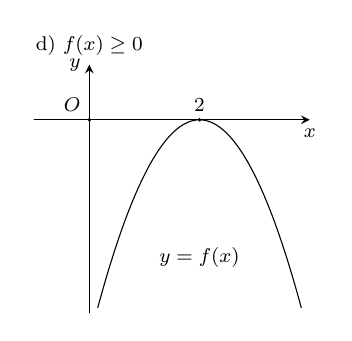
\begin{tikzpicture}[scale=0.7, font=\footnotesize, line join=round, line cap=round, >=stealth]
			\def\ymin{-3.5} \def\ymax{1}
			\def\xmin{-1} \def\xmax{4} 
			\draw[->] (\xmin,0)--(\xmax,0) node [below]{$x$};
			\draw[->] (0,\ymin)--(0,\ymax) node [left]{$y$};
			\fill (0,0)circle(1pt)node[above left]{$O$} (2,0)circle(1pt)node[above]{$2$};
			\draw (0,1)node[above]{d) $f(x)\ge 0$} (2,-2.5)node{ $y=f(x)$};
			\clip (\xmin+0.1,\ymin+0.1) rectangle (\xmax-0.1,\ymax-0.1);
			\draw[smooth,samples=300] plot(\x,{-((\x)-2)^2});
		\end{tikzpicture}
	\end{center}
	\loigiai{
		\begin{enumerate}[a)]
			\item $f(x)<0$ khi và chỉ khi $-\dfrac{7}{3}<x<\dfrac{1}{2}$. Tập nghiệm của bất phương trình là  $\left(-\dfrac{7}{3};\dfrac{1}{2}\right)$.\\
			\item $f(x)>0$ khi và chỉ khi $x \ne -\dfrac{5}{3}$. Tập nghiệm của bất phương trình là $\mathbb{R} \setminus \left\{\dfrac{-5}{3}\right\}$.\\
			\item $f(x) \geq 0$ khi và chỉ khi $x \leq \dfrac{5}{4}$ hoặc $x \geq \dfrac{5}{2}$.\\
			Tập nghiệm của bất phương trình là  $\left(-\infty;\dfrac{5}{4}\right] \cup \left[\dfrac{5}{2};+\infty \right)$.\\
			\item $f(x) \geq 0$ khi và chỉ khi $x=2$. Tập nghiệm của bất phương trình là $\{2\}$.
		\end{enumerate}
	}
\end{bt}

% từ: cau-hoi/lop10/0D7_Bat_phuong_trinh_bac_2_mot_an/0D7-3-6_Toan_hinh_toan_thuc_te_ung_dung_phuong_trinh.tex
\begin{bt}%[0D7C3-6]%[ma:1d2b8cc4]
	Tam giác $ABC$ vuông tại $A$ có điểm $D$ nằm giữa $A$ và $B$. Biết $BC = 8$, $BD = 3$ và $CD = 6$, tính diện tích tam giác $ABC$ (làm tròn đến  chữ số thập phân thứ nhất sau dấu phẩy).
	\shortans{15,7} 
	\loigiai{ 
	 \immini
		{ 
		Đặt $AD = x$ ($x > 0$). Khi đó theo định lý Py-ta-go  ta có
		\begin{itemize}
			\item $AC^2 = CD^2  - AD^2 = 6^2 - x^2 = 36 - x^2$.
			 \item $AC^2 = BC^2 - AB^2 = 8^2 - (x+3)^2 = 55 - 6x - x^2$.
		\end{itemize}
		Do đó  $36 - x^2 = 55 - 6x - x^2 \Leftrightarrow x = \dfrac{19}{6}$, suy ra
		 \[
		S_{ABC} = \dfrac{1}{2}AB\cdot AC = \dfrac{1}{2}(x+3)\sqrt{36-x^2}  \approx 15{,}7.
		\] 
		} 
		 {
		\begin{tikzpicture}[line join=round,line cap = round,>=stealth,scale=.8,font=\footnotesize,transform shape]
				\foreach  \x/\y/\z/\g in
					{ 
					0/0/A/-135,3/0/D/-90,5/0/B/-45,0/4/C/135 
				} 
				\draw[fill=black] (\x,\y) circle  (1pt) coordinate (\z)
					($(\z)+(\g:3.5mm)$) node{$\z$}; 
				\draw  (D)--(C)--(B)--(A)--(C);
			\end{tikzpicture}
		} 
	} 
\end{bt}

% từ: cau-hoi/lop10/0D8_Dai_so_to_hop/0D8-1-2_Bai_toan_chi_su_dung_quy_tac_nhan.tex
\begin{bt}%[0D8H1-2]%[ma:c1839475]
	Cho  các mệnh đề\\
	$A$: \lq\lq Nếu  $\triangle ABC$ đều có cạnh bằng $a$, đường cao là $h$ thì $h = \dfrac{a\sqrt{3}}{2}$\rq\rq.\\
	$B$: \lq\lq Tứ giác có bốn cạnh bằng  nhau là hình vuông\rq\rq.\\
	$C$:  \lq\lq $15$ là số nguyên tố\rq\rq.\\
	$D$: \lq\lq $\sqrt{125}$ là một số  nguyên\rq\rq.\\
	Hãy cho biết trong các mệnh đề kéo theo sau có bao  nhiêu mệnh đề sai?\\
	$A \Rightarrow B$, $B \Rightarrow C$, $A \Rightarrow  D$.
	\shortans{2} 
	\loigiai{ 
		\begin{itemize}
			\item Mệnh đề $A \Rightarrow B$ là sai do  $A$ đúng nhưng $B$ sai.
			\item Mệnh đề $B \Rightarrow  C$ là đúng vì cả $B$ và $C$ đều sai.
			\item Mệnh đề  $A \Rightarrow D$ là sai do $A$ đúng nhưng $D$ sai.
		\end{itemize}
		 Vậy có hai mệnh đề sai.
	} 
\end{bt}

% từ: cau-hoi/lop10/0D8_Dai_so_to_hop/0D8-1-5_Bai_toan_dem_so_tu_nhien.tex
\begin{ex}%[0D8H1-5]%[ma:e67c7a92]
	Cho hai mệnh đề $P$: \lq\lq $ABC$ là tam giác đều\rq\rq\ và mệnh đề $Q$: \lq\lq $ABC$ là  tam giác cân\rq\rq.
	Xét mệnh đề kéo theo \lq\lq Nếu $P$  thì $Q$\rq\rq.
	\choiceTF 
		{\True $P$ là điều kiện  đủ để có $Q$}
		{\True $Q$ là điều kiện cần để  có $P$}
		{\True Mệnh đề  \lq\lq Nếu $P$ thì $Q$\rq\rq\ là mệnh đề đúng}
		 {Mệnh đề \lq\lq Nếu $Q$ thì $P$\rq\rq\ là mệnh đề đúng}
	\loigiai{ 
		Mệnh  đề $P \Rightarrow Q$ được phát biểu: \lq \lq Nếu $ABC$ là tam giác đều thì $ABC$ là tam giác cân\rq \rq.
		\begin{itemchoice}
			\itemch  $P$ là điều kiện đủ để có $Q$.
			\itemch $Q$ là điều kiện cần để có $P$. 
			\itemch Mệnh đề \lq\lq Nếu $P$ thì $Q$\rq\rq\ là mệnh đề đúng vì mọi tam giác đều là tam giác cân. 
			\itemch Không phải  tam giác cân nào cũng là tam giác đều nên mệnh đề \lq\lq Nếu $Q$ thì $P$\rq\rq\ là mệnh đề sai.
		\end{itemchoice}
	} 
\end{ex}

% từ: cau-hoi/lop10/0D8_Dai_so_to_hop/0D8-2-2_Bai_toan_co_bieu_thuc.tex
\begin{ex}%[0D8N2-2]%[ma:5865ac2f]
	Cho tập hợp $X$ gồm $10$ phần tử. Số các hoán vị  của $10$ phần tử của tập hợp $X$ là
	\choice 
		 {$2^{10}$}
		 {$10^{10}$}
		{\True$10!$} 
		 {$10^2$}
	 \loigiai{
		Số các hoán vị  của $10$ phần tử của tập hợp $X$ là $10!$.
	 }
\end{ex}

% từ: cau-hoi/lop10/0D8_Dai_so_to_hop/0D8-3-6_Toan_to_hop_co_dung_nhi_thuc_Newton.tex
\begin{bt}%[0D8C3-6]%[ma:0d8e93b9]
	Cho tập hợp $S$ có $n$  ($n\ge 3 $) phần tử. Gọi $A_1$, $A_2$, $A_3$, $A_4$, $A_5$, $A_6$ là các tập con của tập hợp $S$ thỏa mãn đồng thời
	\begin{itemize}
		\item $\left|A_i\right|=5$, với mọi $1\le i\le  6 $,
		\item $  \left|A_i\cap A_j\right| \le 2$, với mọi $1\le i<j\le 6 $.
	\end{itemize}
	Tìm giá trị nhỏ nhất của  $ n $.
	\shortans{10} 
	\loigiai{ 
		Đặt $ S=\left\{x_1;x_2;\ldots;x_n\right\} $. Ta đếm số bộ $\left(\left\{A_i, A_j\right\}, x_k\right)$, trong đó $x_k \in A_i \cap A_j$ và  $\left\{A_i, A_j\right\}$ không có tính thứ tự. Gọi số bộ này là $T$.\\
		Đếm theo  cặp tập hợp $\left(A_i, A_j\right)$, ta có $T \le 2 \mathrm{C}_6^2=30$.\\
		Đếm phần tử $x$. Gọi  $a_i$ là số tập hợp chứa phần tử $x_i$ với mọi $i=\overline{1, n}$. Khi đó, đếm theo số phần tử, ta có $a_1+a_2+\ldots+a_n=6\cdot 5=30$. Ngoài ra,
		$$ 
		T=\displaystyle \sum_{i=1}^n \mathrm{C}_{a_1}^2=\dfrac{1}{2}\left(a_1^2+a_2^2+\ldots+a_n^2-30\right) \ge  \dfrac{1}{2}\left[\dfrac{\left(a_1+a_2+\ldots+a_n\right)^2}{n}-30\right]=\dfrac{1}{2}\left(\dfrac{900}{n}-30\right).$$
		Suy ra $\dfrac{1}{2}\left(\dfrac{900}{n}-30\right)  \le 30 \Rightarrow n \ge 10$.\\
		Với $n=10$, ta có bảng sau  (ô được đánh dấu $x$ nghĩa là phần tử $x_{i} \in A_{j}$):
		\begin{center}
			\begin{tabular}{|c|c|c|c|c|c|c|c|c|c|c|}
				\hline & $\mathrm{x}_1$ & $\mathrm{x}_2$ & $\mathrm{x}_3$ & $\mathrm{x}_4$ & $\mathrm{x}_5$ & $\mathrm{x}_6$  & $\mathrm{x}_7$ & $\mathrm{x}_8$ & $\mathrm{x}_9$ & $\mathrm{x}_{10}$ \\
				\hline $A_1$ &  $\mathrm{x}$ & $\mathrm{x}$ & $\mathrm{x}$ & $\mathrm{x}$ & $\mathrm{x}$ & & & & & \\
				\hline $A_2$ & $\mathrm{x}$ & $\mathrm{x}$ & & & & $\mathrm{x}$ & $\mathrm{x}$ & $\mathrm{x}$ & &  \\
				\hline $A_3$ & $\mathrm{x}$ & & $\mathrm{x}$ & & & $\mathrm{x}$  & & & $\mathrm{x}$ & $\mathrm{x}$ \\
				\hline $A_4$ & & $\mathrm{x}$ & &  $\mathrm{x}$ & & & $\mathrm{x}$ & & $\mathrm{x}$ & $\mathrm{x}$ \\
				\hline $A_5$ & & & & $\mathrm{x}$ & $\mathrm{x}$ & $\mathrm{x}$ & & $\mathrm{x}$  & $\mathrm{x}$ & \\
				\hline $A_6$ & & & $\mathrm{x}$ & & $\mathrm{x}$ & & $\mathrm{x}$ & $\mathrm{x}$  & & $\mathrm{x}$ \\
				\hline 
			\end{tabular}
		\end{center}
		Vậy giá trị nhỏ nhất của $n$  là $10$.
	 }
\end{bt}

% từ: cau-hoi/lop10/0H4_He_thuc_luong_trong_tam_giac/0H4-2-1_Bai_toan_chi_dung_dinh_ly_Sin_Cosin.tex
\begin{bt}%[0H4H2-1]%[Phạm Tuấn]%[ma:4276af22]
    \immini{
        Cho tam giác $A B C$ có $AB=20$, $AC=15$, $\widehat{A}=60^{\circ}$. Tính cạnh $BC$ và các góc $B$, $C$  của tam giác đó (làm tròn kết quả đến hàng phần mười).
    }
    {
        \begin{tikzpicture}[scale=1, font=\footnotesize, line join=round, line cap=round,>=stealth]
            \path
            (0,0) coordinate (A)
            (4,0) coordinate (B)
            ;
            \coordinate (C) at ($(A)+(60:3)$) ; 
            \draw (A)--(B)--(C)--(A) 
            pic["$60^{\circ}$", draw=black, angle eccentricity=1.5, angle radius=0.7cm]{angle=B--A--C}; 
            \foreach \x/\g in {A/-120,B/-60,C/90} 
            \fill[black] (\x) circle (1pt)+(\g:3mm) node {$\x$};
        \end{tikzpicture}
    }
    \loigiai{
        Áp dụng định lí côsin ta có 
        \[ BC^2=AB^2+AC^2-2AB \cdot AC \cos A =20^2+15^2-2 \cdot 20 \cdot 15 \cos 60^\circ  =  325\Rightarrow BC=\sqrt{325} \approx 18.\]
        Áp dụng định lí sin ta có 
        \begin{align*}
            \dfrac{AC}{\sin B} = \dfrac{BC}{\sin A} \Rightarrow \sin B = \dfrac{AC\sin A}{BC}  = \dfrac{15 \sin 60^{\circ}}{\sqrt{325}} \Rightarrow B \approx 46{,}1^\circ.  
        \end{align*}
        Khi đó $\widehat{C}= 180^\circ - \widehat{A} - \widehat{B} =  180^\circ  -60^\circ - 46{,}1^\circ= 73{,}9^\circ$.
    }
\end{bt}

% từ: cau-hoi/lop10/0H4_He_thuc_luong_trong_tam_giac/0H4-2-1_Bai_toan_chi_dung_dinh_ly_Sin_Cosin.tex
\begin{bt}%[0H4H2-1]%[Phạm Tuấn]%[ma:611c79a5]
    \immini{
        Cho tam giác $A B C$ có $AB=12$, $AC=9$, $\widehat{A}=60^{\circ}$. $M$ là điểm thuộc cạnh $AB$  sao cho $AM=2BM$. Tính cạnh $CM$ và  góc $\widehat{BCM}$ (làm tròn kết quả đến hàng phần mười).
    }
    {
        \begin{tikzpicture}[scale=1, font=\footnotesize, line join=round, line cap=round,>=stealth]
            \path
            (0,0) coordinate (A)
            (4,0) coordinate (B)
            ;
            \coordinate (M) at ($(A)!{2/3}!(B)$) ;
            \coordinate (C) at ($(A)+(60:3)$) ; 
            \draw (A)--(B)--(C)--(A) (C)--(M) 
            pic["$60^{\circ}$", draw=black, angle eccentricity=1.5, angle radius=0.7cm]{angle=B--A--C};
            \foreach \x/\g in {A/-120,B/-60,C/90,M/-90} 
            \fill[black] (\x) circle (1pt)+(\g:3mm) node {$\x$};
        \end{tikzpicture}
    }
    \loigiai{
        Ta có $AM=2BM \Rightarrow BM = \dfrac{1}{3}AB=4$ và $AM=\dfrac{2}{3}AB=8$. \\
        Áp dụng định lí côsin ta có 
        \begin{align*}
            &CM^2=AM^2+AC^2-2AM \cdot AC \cos A =8^2+9^2-2 \cdot 8 \cdot 9 \cos 60^\circ  =  73 \Rightarrow CM=\sqrt{73} \approx 8{,}5; \\
            &BC^2=AB^2+AC^2-2AB \cdot AC \cos A =12^2+9^2-2 \cdot 12 \cdot 9 \cos 60^\circ  =  117\Rightarrow BC=\sqrt{117}.
        \end{align*}
        Áp dụng định lí côsin ta có 
        \begin{align*}
            &BM^2=CM^2+CB^2-2CM \cdot CB \cos \widehat{BCM}  \\
            \Leftrightarrow~ & \cos \widehat{BCM} = \dfrac{CM^2+CB^2- BM^2}{2CM \cdot CB}  \\
            \Leftrightarrow~ & \cos \widehat{BCM} = \dfrac{73+117-16}{2 \cdot \sqrt{73} \cdot \sqrt{117}} =  \dfrac{29}{\sqrt{949}}\\
            \Rightarrow~& \widehat{BCM} \approx 19{,}7^\circ. 
        \end{align*}
    }
\end{bt}

% từ: cau-hoi/lop10/0H4_He_thuc_luong_trong_tam_giac/0H4-3-1_Giai_tam_giac.tex
\begin{bt}%[0H4H3-1]%[ma:28668c45]
    Cho tam giác $ABC$ có $\widehat{A}=100^{\circ}$, $\widehat{C}=35^{\circ}$ và $b=10$. Tính $a$, $c$, $R$ và số đo góc $B$.
    \loigiai{
        Ta có $\widehat{B}=180^{\circ}-\left(\widehat{A}+\widehat{C}\right)=180^{\circ}-\left(100^{\circ}+35^{\circ}\right)=45^{\circ}$.\\
        Áp dụng Định lí sin, ta có $\dfrac{a}{\sin 100^{\circ}}=\dfrac{10}{\sin 45^{\circ}}=\dfrac{c}{\sin 35^{\circ}}=2R$.\\
        Suy ra $\heva{&a=\dfrac{10}{\sin 45^{\circ}}\cdot\sin 100^{\circ}=10\sqrt{2}\cdot\sin 100^{\circ}\approx 13{,}93\\&c=\dfrac{10}{\sin 45^{\circ}}\cdot\sin 35^{\circ}=10\sqrt{2}\cdot\sin 35^{\circ}\approx 8{,}11\\&R=\dfrac{10}{2\sin 45^{\circ}}=5\sqrt{2}.}$
    }
\end{bt}

% từ: cau-hoi/lop10/0H4_He_thuc_luong_trong_tam_giac/0H4-3-1_Giai_tam_giac.tex
\begin{bt}%[0H4H3-1][Dự án đề kiểm tra HKI NH22-23- Tên Phạm Văn Long]%[THPT-TRƯỜNG-CHINH-2]%[ma:d3cee5f6]
	Cho tam giác $ABC$ có $AB=4$, $BC=5$, $\widehat{B}=60^\circ$. Tính độ dài cạnh $AC$, diện tích tam giác $ABC$, bán kính đường tròn ngoại tiếp và bán kính đường tròn nội tiếp của tam giác $ABC$.
	\loigiai{
		Ta có 
		\begin{itemize}
			\item $AC=\sqrt{AB^2+BC^2-2\cdot AB\cdot BC\cdot \sin  B}=\sqrt{4^2+5^2-2\cdot 4\cdot 5\cdot \cos  60^\circ}=\sqrt{21}$.
			\item $S_{\triangle ABC}=\dfrac{1}{2}\cdot AB\cdot BC\sin B=\dfrac{1}{2}\cdot4\cdot 5\sin 60^\circ=5\sqrt{3}$.
			\item $\dfrac{AC}{\sin B}=2R\Rightarrow R=\dfrac{AC}{2\sin B}=\dfrac{\sqrt{21}}{2\sin 60^\circ}=\sqrt{7}$.
			\item $S=p\cdot r\Rightarrow r=\dfrac{S}{p}=\dfrac{5\sqrt{3}}{(4+5+\sqrt{21}):2}=\dfrac{3\sqrt{3}-\sqrt{7}}{2}$.
		\end{itemize}
		
	}
\end{bt}

% từ: cau-hoi/lop10/0H5_Vecto_chua_xet_toa_do/0H5-2-1_Tinh_toan_thu_gon_hieu_cac_vecto.tex
\begin{bt}%[0H5N2-1]%[Dự án 4 - TLDH - TeamTeXHoa - Lê Quân]%[ma:4be064ae]
Cho tam giác $ABC$. Gọi $M,\,N,\,P$ lần lượt là trung điểm của $BC,\,CA,\,AB$.
\begin{enumerate}
\item Xác định các véc-tơ khác véc-tơ-không cùng phương với $\overrightarrow{MN}$ có điểm đầu và điểm cuối lấy trong các điểm đã cho.
\item Xác định các véc-tơ khác véc-tơ-không cùng hướng với $\overrightarrow{AB}$ có điểm đầu và điểm cuối lấy trong điểm đã cho.
\item Vẽ các véc-tơ bằng véc-tơ $\overrightarrow{NP}$ mà có điểm đầu $A,\,B$.
\end{enumerate}
\loigiai{
\immini{
\begin{enumerate}
\item Các véc-tơ khác véc-tơ không cùng phương với $\overrightarrow{MN}$ là $\overrightarrow{NM},\,\overrightarrow{AB},\,\overrightarrow{BA},\,\overrightarrow{AP},\,\overrightarrow{PA},\,\overrightarrow{BP},\,\overrightarrow{PB}$.
\item Các véc-tơ khác véc-tơ-không cùng hướng với $\overrightarrow{AB}$ là $\overrightarrow{AP},\,\,\overrightarrow{PB},\,\,\overrightarrow{NM}$ .
\item Trên tia $CB$ lấy điểm $B'$ sao cho $BB'=NP$.\\
Khi đó ta có $\overrightarrow{BB'}$ là véc-tơ có điểm đầu là $B$ và bằng véc-tơ $\overrightarrow{NP}$.\\
Qua $A$ dựng đường thẳng song song với đường thẳng $NP$. Trên đường thẳng đó lấy điểm $A'$ sao cho $\overrightarrow{AA'}$ cùng hướng với $\overrightarrow{NP}$ và $AA'=NP$.\\
Khi đó ta có $\overrightarrow{AA'}$ là véc-tơ có điểm đầu là $A$ và bằng véc-tơ $\overrightarrow{NP}$.
\end{enumerate}}
{\begin{tikzpicture}[line join=round, line cap=round,thick, scale=.7]
	\coordinate (A) at (0,3);
	\coordinate (B) at (-2,0);
	\coordinate (C) at (3,0);
	\draw(A)--(B)--(C)--cycle;
	\coordinate (P) at ($(A)!0.5!(B)$);
	\coordinate (N) at ($(A)!0.5!(C)$);
	\coordinate (M) at ($(C)!0.5!(B)$);
	\coordinate (B') at ($(B)+(P)-(N)$);
		\coordinate (A') at ($(A)+(P)-(N)$);
		\draw(M)--(N)--(P)--cycle;
		\draw[->] (B)--(B');
		\draw[->] (A)--(A');
	\foreach \i/\g in {A/90, A'/90, B'/90, M/-90, P/180, B/-90,C/-90, N/30}{\draw[fill=black](\i) circle (1.5pt) ($(\i)+(\g:5mm)$) node[scale=1]{$\i$};}
\end{tikzpicture}}

}
\end{bt}

% từ: cau-hoi/lop10/0H9_Phuong_phap_toa_do_trong_mat_phang/0H9-2-2_Tim_goc_nho_tich_vo_huong.tex
\begin{bt}%[0H9B2-2]%[0H9B3-2]%[ma:281fb5f1]
	Cho $A(2;-1)$; $B(4;  3)$; $C(-5; 0)$
	\begin{listEX}
		\item Viết phương trình tổng quát  đường thẳng đi qua $2$ điểm $A$ và $C$.
		 \item Viết phương trình đường tròn tâm $B$ và tiếp xúc với đường thẳng $AC$.
	\end{listEX}
	 \loigiai{
		\begin{listEX}
			\item Đường thẳng $AC$ có véc-tơ chỉ phương $\overrightarrow{A C}=(-7;  1)$.\\
			Suy  ra đường thẳng $AC$ qua $A$, có véc-tơ pháp tuyến $\overrightarrow{n}=(1; 7)$ có phương trình
			\[1\cdot (x-2)+7\cdot (y+1)=0 \Leftrightarrow x+7y+5=0  \]
			\item Ta có đường tròn tâm $B$ và tiếp xúc với đường thẳng  $AC$ nên
			\[R=\mathrm{d}\,(B,AC)=\dfrac{|4+7 \cdot 3+5|}{\sqrt{1^2+7^2}}=\dfrac{30}{\sqrt{50}}=3 \sqrt{2}.\] 
			Suy ra đường tròn $(C)$ có tâm $B$,  bán kính $R=3 \sqrt{2}$ có phương trình
			 \[(C)\colon (x-4)^2+(y-3)^2=18.\]
		\end{listEX}
	} 
\end{bt}

% từ: cau-hoi/lop10/0H9_Phuong_phap_toa_do_trong_mat_phang/0H9-3-2_Phuong_trinh_duong_thang.tex
\begin{bt}%[0H9H3-2]%[Tex hóa SGK CD,T8/22, Phạm Doãn Lê Bình]%[ma:5c4d0941]
	Lập phương trình mỗi đường thẳng trong các hình dưới đây
	\begin{center}
		\begin{tikzpicture}[scale=0.7, font=\footnotesize, line join=round, line cap=round, >=stealth,x=0.7cm,y=0.7cm]
			\draw[->](0,-1.5)--(0,5.5) node[left]{$y$};
			\draw[->](-2.5,0)--(5.5,0) node[below]{$x$};
			\draw (0,0) node [below left] {$O$};
			\foreach \x in {-2,-1,1,2,3,4,5}
			\draw[shift={(\x,0)},color=black] (0pt,2pt) -- (0pt,-2pt);
			\foreach \y in {-1,1,2,3,4,5}
			\draw[shift={(0,\y)},color=black] (2pt,0pt) -- (-2pt,0pt);
			\draw (1,0) node[below]{$1$} (3,0) node[below]{$3$}
			(0,1) node[left]{$1$}  (0,4) node[left]{$4$};
			\draw[samples=100,smooth,domain=-0.9:4] plot (\x,{-4/3*(\x)+4});
			\draw (0.7,-2.3) node{Hình 1};
		\end{tikzpicture} 
		\hspace{1cm}
		\begin{tikzpicture}[scale=0.7, font=\footnotesize, line join=round, line cap=round, >=stealth,x=0.7cm,y=0.7cm]
			\draw[->](0,-2.5)--(0,5.5) node[left]{$y$};
			\draw[->](-3.5,0)--(5,0) node[below]{$x$};
			\draw (0,0) node [below left] {$O$};
			\foreach \x in {-3,-2,-1,1,2,3,4}
			\draw[shift={(\x,0)},color=black] (0pt,2pt) -- (0pt,-2pt);
			\foreach \y in {-2,-1,1,2,3,4,5}
			\draw[shift={(0,\y)},color=black] (2pt,0pt) -- (-2pt,0pt);
			\draw (1,0) node[below]{$1$} (2,0) node[below]{$2$} (-2,0) node[above]{$-2$}
			(0,1) node[left]{$1$}  (0,4) node[left]{$4$}  (0,-2) node[right] {$-2$};
			\draw[samples=100,smooth,domain=-2.1:2.9] plot (\x,{1.5*(\x)+1});
			\draw[dashed] (-2,0)--(-2,-2)--(0,-2)  (2,0)--(2,4)--(0,4);
			\draw (0,-3) node{Hình 2};
		\end{tikzpicture} \\
		\begin{tikzpicture}[scale=0.7, font=\footnotesize, line join=round, line cap=round, >=stealth,x=0.7cm,y=0.7cm]
			\draw[->](0,-1.5)--(0,5.5) node[left]{$y$};
			\draw[->](-3.5,0)--(2.5,0) node[below]{$x$};
			\draw (0,0) node [below left] {$O$};
			\foreach \x in {-3,-2,-1,1,2}
			\draw[shift={(\x,0)},color=black] (0pt,2pt) -- (0pt,-2pt);
			\foreach \y in {-1,1,2,3,4,5}
			\draw[shift={(0,\y)},color=black] (2pt,0pt) -- (-2pt,0pt);
			\draw (1,0) node[below]{$1$} 
			(0,1) node[left]{$1$} ;
			\draw (-2.5,-1.5)--(-2.5,5);
			\draw[fill=black] (-2.5,0) circle (1pt) node[below left]{$-\frac{5}{2}$};
			\draw (0,-2) node{Hình 3};
		\end{tikzpicture} 
		\hspace{1cm}
		\begin{tikzpicture}[scale=0.7, font=\footnotesize, line join=round, line cap=round, >=stealth,x=0.7cm,y=0.7cm]
			\draw[->](0,-1.5)--(0,5.5) node[left]{$y$};
			\draw[->](-4.5,0)--(4.5,0) node[below]{$x$};
			\draw (0,0) node [below left] {$O$};
			\foreach \x in {-4,-3,-2,-1,1,2,3,4}
			\draw[shift={(\x,0)},color=black] (0pt,2pt) -- (0pt,-2pt);
			\foreach \y in {-1,1,2,3,4,5}
			\draw[shift={(0,\y)},color=black] (2pt,0pt) -- (-2pt,0pt);
			\draw (1,0) node[below]{$1$} 
			(0,1) node[left]{$1$} (0,3) node[above left]{$3$};
			\draw (-4,3)--(4,3);
			\draw (0,-2) node{Hình 4};
		\end{tikzpicture} 
	\end{center}
	\loigiai{
		\begin{itemize}
			\item[$\bullet$] Đường thẳng ở hình $1$ đi qua hai điểm $(0;4)$ và $(3;0)$ nên có phương trình là \[ \dfrac{x}{3}+\dfrac{y}{4}=1 \Leftrightarrow 4x+3y-12=0.\]
			\item[$\bullet$] Đường thẳng ở hình $2$ đi qua hai điểm $(-2;-2)$ và $(2;4)$ nên có phương trình là 
			\[ \dfrac{x+2}{2+2} = \dfrac{y+2}{4+2}\Leftrightarrow 3x-2y+2=0.\]
			\item[$\bullet$] Đường thẳng ở hình $3$ là đường thẳng song song với trục $Oy$ và cắt trục $Ox$ tại điểm có hoành độ $x=-\dfrac{5}{2}$ nên đường thẳng đó có phương trình là
			\[ x=-\dfrac{5}{2}\Leftrightarrow 2x+5=0.\]
			\item[$\bullet$] Đường thẳng ở hình $4$ là đường thẳng song song với trục $Ox$ và cắt trục $Oy$ tại điểm có tung độ $y=3$ nên đường thẳng đó có phương trình là
			\[ y=3\Leftrightarrow y-3=0.\]
		\end{itemize}
	}
\end{bt}

% từ: cau-hoi/lop10/0H9_Phuong_phap_toa_do_trong_mat_phang/0H9-3-5_Bai_toan_ve_khoang_cach.tex
\begin{bt}%[0H9V3-5]%[ma:b3d20e66]
	Trong mặt phẳng toạ độ, cho tam giác $ABC$ có $A(1; 0), B(3 ; 2)$ và $C(-2 ;-1)$.
	\begin{enumerate}
		\item Tính độ dài đường cao kẻ từ đỉnh $A$ của tam giác $ABC$.
		\item Tính diện tích tam giác $ABC$. 
	\end{enumerate}
	\loigiai{
		\begin{enumerate}
			\item Đường thẳng $BC$ qua $B(3; 2)$ và nhận $\overrightarrow{BC}=(-5; -3)$ làm véc-tơ chỉ phương nên có véc-tơ pháp tuyến là $\overrightarrow{n}=(3; -5)$. Suy ra đường thẳng $BC$ có phương trình $3(x-3)-5(y-2)=0\Leftrightarrow 3x-5y-1=0$.\\
			Độ dài đường cao kẻ từ đỉnh $A$ của $\triangle ABC$ chính bằng $\mathrm{d}(A,BC)=\dfrac{2}{\sqrt{34}}$.
			\item Ta có $BC=\sqrt{34}$, suy ra diện tích tam giác $ABC$ là $$S_{\triangle ABC}=\dfrac{1}{2}BC\cdot \mathrm{d}(A,BC)=\dfrac{1}{2}\cdot \sqrt{34}\cdot\dfrac{2}{\sqrt{34}}=1.$$ 
		\end{enumerate}
		
	}
\end{bt}

% từ: cau-hoi/lop10/0H9_Phuong_phap_toa_do_trong_mat_phang/0H9-4-1_Tim_tam_ban_kinh_va_dieu_kien_la_duong_tron.tex
\begin{bt}%[0H9H4-1] Tìm tâm và bán kính của đường tròn $(C)$ trong các trường hợp sau:%[ma:4674589a]
\begin{enumEX}{2}
\item $(x-2)^2+(y-8)^2=49$;
\item $(x+3)^2+(y-4)^2=23$.
\end{enumEX}
\loigiai{
\begin{listEX}[1]
\item Từ phương trình đường tròn ta có tâm $I(2;8)$, bán kính $R=7$.
\item Từ phương trình đường tròn ta có tâm  $I(-3;4)$, bán kính $R=\sqrt{23}$.
\end{listEX}
}
\end{bt}

% từ: cau-hoi/lop11/1D1_Ham_so_luong_giac_va_phuong_trinh_luong/1D1-1-1_Cau_hoi_ly_thuyet.tex
\begin{bt}%[1D1B1-1]%[ma:41ff1336]
	 Tìm tập xác định $\mathscr{D}$ của hàm số
	$y=\dfrac{2\tan  2x-5}{\sin 2x+1}$.
	 \loigiai{
		Điều kiện: \\ 
		$\heva{&\sin 2x+1\neq 0\\& \cos 2x\neq 0}\Leftrightarrow \heva{&\sin 2x\neq -1\\& \cos 2x\neq 0}\Leftrightarrow \heva{& 2x\neq -\dfrac{\pi}{2}  +k2\pi\\&2x\neq \dfrac{\pi}{2}+k\pi}\Leftrightarrow \heva{& x\neq -\dfrac{\pi}{4} +k\pi\\&x\neq \dfrac{\pi}{4}+k\dfrac{\pi}{2}}\Leftrightarrow x\neq \dfrac{\pi}{4}+k\dfrac{\pi}{2}$.\\
		Tập xác định $\mathscr{D}=\mathbb{R}\setminus\left\lbrace  \dfrac{\pi}{4}+k\dfrac{\pi}{2}, \, k\in \mathbb{Z} \right\rbrace$.\\
	 }
\end{bt}

% từ: cau-hoi/lop11/1D1_Ham_so_luong_giac_va_phuong_trinh_luong/1D1-1-1_Cau_hoi_ly_thuyet.tex
\begin{bt}%[1D1K1-1]%[ma:1b9c86ee]
	Tìm tập  xác định $\mathscr{D}$ của hàm số
	$y=\dfrac{1}{\sin x}+\dfrac{1}{\cos x}$. 
	\loigiai{ 
		 Điều kiện: $\heva{&\cos x\neq 0\\& \sin x\neq 0}\Leftrightarrow \heva{& x\neq k\pi\\&x\neq \dfrac{\pi}{2}+k\pi}\Leftrightarrow x\neq k\dfrac{\pi}{2}.$\\
		Tập xác định $\mathscr{D}=\mathbb{R}\setminus\left\lbrace k\dfrac{\pi}{2},\, k\in \mathbb{Z} \right\rbrace$.\\ 
	} 
\end{bt}

% từ: cau-hoi/lop11/1D1_Ham_so_luong_giac_va_phuong_trinh_luong/1D1-1-3_So_do_cua_mot_goc_luong_giac.tex
\begin{ex}%[1D1B1-3]%[ma:94ec45cd]
	Cho hai hàm số  $f(x)=\sin2x$ và $g(x)=\cos3x$. Mệnh đề nào sau đây là đúng?
	\choice 
		 {$f(x)$ và $g(x)$ là hai hàm số chẵn}
		{$f(x)$ và  $g(x)$ là hai hàm số lẻ}
		{$f(x)$ là  hàm số chẵn và $g(x)$ là hàm số lẻ}
		{\True $f(x)$ là hàm số lẻ  và $g(x)$ là hàm số chẵn}
	\loigiai{ 
	\begin{itemize}
		\item Xét hàm số $f(x)=\sin  2x$.\\
		Tập  xác định là $\mathscr{D}=\mathbb{R}$.\\
		Với mọi  $x\in\mathscr{D}$ thì $-x\in \mathscr{D}$; $f(-x)=\sin(-2x)=-\sin 2x=-f(x)$.\\
		Vậy hàm số $f(x)=\sin 2x$ là hàm số lẻ. 
		 \item Xét hàm số $f(x)=\cos 3x$.\\
		Tập xác định  là $\mathscr{D}=\mathbb{R}$.\\
		Với mọi $x\in\mathscr{D}$ thì  $-x\in \mathscr{D}$; $f(-x)=\cos(-3x)=\cos 3x=f(x)$.\\
		Vậy hàm số $f(x)=\cos 3x$ là  hàm số chẵn.
	\end{itemize}
	} 
\end{ex}

% từ: cau-hoi/lop11/1D1_Ham_so_luong_giac_va_phuong_trinh_luong/1D1-2-1_Cau_hoi_ly_thuyet.tex
\begin{ex}%[1D1B2-1]%[ma:7879be5f]
	Nghiệm của phương trình $ 2\cos \dfrac{x}{2}+\sqrt{3}=0$ là 
	 \choice
		{$  x=\pm\dfrac{5\pi}{6}+k2\pi ,k\in\mathbb{Z} $}
		{\True  $ x=\pm\dfrac{5\pi}{3}+k4\pi ,k\in\mathbb{Z}$}
		 {$x=\pm\dfrac{5\pi}{3}+k2\pi ,k\in\mathbb{Z} $}
		{$x=\pm\dfrac{5\pi}{6}+k4\pi ,k\in\mathbb{Z} $} 
	 \loigiai{
		Phương trình tương đương với $$\cos  \dfrac{x}{2}=-\dfrac{\sqrt{3}}{2}\Leftrightarrow\dfrac{x}{2}=\pm \dfrac{5\pi}{6}+k2\pi\Leftrightarrow x=\pm\dfrac{5\pi}{3}+k4\pi,\,k\in\mathbb{Z}.$$
	 }
\end{ex}

% từ: cau-hoi/lop11/1D1_Ham_so_luong_giac_va_phuong_trinh_luong/1D1-2-1_Cau_hoi_ly_thuyet.tex
\begin{ex}%[1D1Y2-1]%[ma:17a8e0bd]
	Giải  phương trình $ 2\cos x-1=0 $.
	\choice 
		{$x=\pm  \dfrac{\pi}{3}+2\pi, k\in \mathbb{Z} $}
		{\True $x=\pm \dfrac{\pi}{3}+k2\pi, k\in \mathbb{Z} $} 
		{$x=\pm  \dfrac{\pi}{6}+k2\pi, k\in \mathbb{Z} $}
		{$x=  \dfrac{\pi}{3}+k2\pi, k\in \mathbb{Z} $}
	 \loigiai{
		Ta có $ 2\cos x-1=0  \Leftrightarrow \cos x=\dfrac{1}{2}\Leftrightarrow x=\pm \dfrac{\pi}{3}+k2\pi, k\in \mathbb{Z}$.
	 }
\end{ex}

% từ: cau-hoi/lop11/1D1_Ham_so_luong_giac_va_phuong_trinh_luong/1D1-2-1_Cau_hoi_ly_thuyet.tex
\begin{ex}%[1D1Y2-1]%[ma:44439d63]
	 Nghiệm của phương trình $\sin x=\dfrac{1}{2}$ là
	 \choice
		{$x=\pm \dfrac{\pi}{6}+k2\pi$} 
		{\True $x=\dfrac{\pi}{6}+k2\pi$  và $x=\dfrac{5\pi}{6}+k2\pi$}
		{$x=\dfrac{\pi}{6}+k\pi$ và $x=\dfrac{5\pi}{6}+k\pi$} 
		{$x=-\dfrac{\pi}{6}+k2\pi$ và $x=-\dfrac{5\pi}{6}+k2\pi$} 
	\loigiai{ 
		 $$\sin x=\dfrac{1}{2}
		\Leftrightarrow \sin x= \sin \dfrac{\pi}{6} 
		\Leftrightarrow  \hoac{&x=\dfrac{\pi}{6}+k2\pi\\&x=\dfrac{5\pi}{6}+k2\pi.}$$
	} 
\end{ex}

% từ: cau-hoi/lop11/1D1_Ham_so_luong_giac_va_phuong_trinh_luong/1D1-2-1_Cau_hoi_ly_thuyet.tex
\begin{ex}%[1D1Y2-1]%[ma:31089cc6]
	Tập nghiệm  của phương trình $\sin 2x=\sin x$ là
	 \choice
		{$S=\left\{k2\pi;\pi+k2\pi\left|k\in  \mathbb{Z}\right. \right\}$}
		{\True $S=\left\{k2\pi;\dfrac{\pi}{3}+\dfrac{k2\pi}{3}\left|k\in \mathbb{Z}\right. \right\}$} 
		{$S=\left\{k2\pi;\dfrac{\pi}{3}+k2\pi\left|k\in \mathbb{Z}\right. \right\}$} 
		{$S=\left\{k2\pi;-\dfrac{\pi}{3}+k2\pi\left|k\in \mathbb{Z}\right.  \right\}$}
	 \loigiai{
		Ta có $\sin 2x=\sin  x \Leftrightarrow \left[
		\begin{aligned}
			 &2x=x+k2\pi \\
			&2x=\pi-x+k2\pi 
		\end{aligned}\right. \Leftrightarrow \left[
		\begin{aligned}
			&x=k2\pi \\ 
			 &x=\dfrac{\pi}{3}+\dfrac{k2\pi}{3}
	\end{aligned}\right. \left(k\in \mathbb{Z}\right)$.}
\end{ex}

% từ: cau-hoi/lop11/1D1_Ham_so_luong_giac_va_phuong_trinh_luong/1D1-2-1_Cau_hoi_ly_thuyet.tex
\begin{ex}%[1D1B2-1]%[ma:728e01ef]
	Phương trình $\sin^2  x+\cos 2x=-\cos^2 x$ có nghiệm là
	 \choice
		{$x=k2\pi, (k\in  \mathbb{Z})$}
		 {$x=\pi+k2\pi, (k\in \mathbb{Z})$}
		 {\True $x=\dfrac{\pi}{2}+k\pi, (k\in \mathbb{Z})$}
		 {$x=k\pi, (k\in \mathbb{Z})$}
	 \loigiai{
		$\sin^2 x+\cos 2x=-\cos^2 x\Leftrightarrow 1+\cos 2x =0 \Leftrightarrow \cos^2 x=0 \Leftrightarrow  x=\dfrac{\pi}{2}+k\pi, (k\in \mathbb{Z})$.
	 }
\end{ex}

% từ: cau-hoi/lop11/1D1_Ham_so_luong_giac_va_phuong_trinh_luong/1D1-2-1_Cau_hoi_ly_thuyet.tex
\begin{ex}%[1D1B2-1]%[ma:1107c056]
	Phương trình lượng giác $2\sin  x+\sqrt{2}=0$ có nghiệm là
	 \choice
		{$\hoac{&x=\dfrac{3\pi}{4}+k2\pi\\&x=\dfrac{\pi}{4}+k2\pi},k\in \mathbb{Z}$} 
		{$\hoac{&x=\dfrac{\pi}{4}+k2\pi\\&x=-\dfrac{\pi}{4}+k2\pi},k\in  \mathbb{Z}$}
		 {\True $\hoac{&x=-\dfrac{\pi}{4}+k2\pi\\&x=\dfrac{5\pi}{4}+k2\pi},k\in \mathbb{Z}$}
		{$\hoac{&x=\dfrac{5\pi}{4}+k2\pi\\&x=\dfrac{\pi}{4}+k2\pi},k\in \mathbb{Z}$} 
	 \loigiai{
		Ta có $2\sin x+\sqrt{2}=0\Leftrightarrow \sin x  =-\dfrac{\sqrt{2}}{2}\Leftrightarrow \hoac{&x=-\dfrac{\pi}{4}+k2\pi\\&x=\dfrac{5\pi}{4}+k2\pi},k\in \mathbb{Z}.$
	} 
\end{ex}

% từ: cau-hoi/lop11/1D1_Ham_so_luong_giac_va_phuong_trinh_luong/1D1-2-2_Xet_dau_gia_tri_luong_giac_Tinh_gia_tri_luong.tex
\begin{ex}%[1D1H2-2]%[ma:45154d98]
	Tìm khẳng định {\bf sai} trong  các khẳng định sau đây?
	\choice 
		{$\tan 45^\circ <\tan 60^\circ  $}
		{$\cos 45^\circ\le\sin 45^\circ  $}
		{$\sin  60^\circ <\sin 80^\circ $}
		{\True $\cos 35^\circ  >\cos 10^\circ $}
	\loigiai{Khi $\alpha\in\left(0^\circ\,;\,90^\circ\right)$ hàm $\cos\alpha $ là hàm giảm nên $\cos  35^\circ <\cos 10^\circ $ suy ra $\cos 35^\circ >\cos 10^\circ $ sai.}
\end{ex}

% từ: cau-hoi/lop11/1D1_Ham_so_luong_giac_va_phuong_trinh_luong/1D1-3-2_Ap_dung_cong_thuc_cong.tex
\begin{bt}%[1D1H3-2]%[ma:798f1b65]
% nguon: Archive/SP_KhoLatex/ID6_old/1.3.1.tex #3110
%::Cau 7::
	\immini{
		Cho tam giác $ABC$ vuông tại $A$ có $AB=4,AC=1$. Trên tia đối của tia $CA$ lấy điểm $D$ sao cho $\widehat{CBD}=45^\circ $. Tính tan $\widehat{ABD}$ và độ dài cạnh $AD$.}
	{\begin{tikzpicture}[line join = round, line cap = round, scale=.6] 
			\coordinate (A) at (0,0);
			\coordinate (B) at (0,6);	
			\coordinate (C) at (1.5,0);
			\coordinate (D) at (8,0); 
			\draw (A)--(B)--(D)--cycle (B)--(C); 
			\foreach \x/\g in {A/180,B/90,C/-90,D/0}\fill[black](\x) circle (2pt)($(\x)+(\g:3.5mm)$) node{$\x$};
		\end{tikzpicture} 
	}
	\loigiai{
		Ta có $\tan \widehat{ABC}=\dfrac{AC}{AB}=\dfrac{1}{4}$.\\
		$\tan \widehat{ABD}=\tan \left( \widehat{ABC}+\widehat{CBD} \right)=\dfrac{\tan \widehat{ABC}+\tan \widehat{CBD}}{1-\tan \widehat{ABC}\cdot\tan \widehat{CBD}}=\dfrac{\dfrac{1}{4}+\tan 45^\circ}{1-\dfrac{1}{4}\cdot\tan 45^\circ}=\dfrac{5}{3}$.\\
		$\tan \widehat{ABD}=\dfrac{AD}{AB}\Rightarrow AD=AB\cdot\tan \widehat{ABD}=4\cdot\dfrac{5}{3}=\dfrac{20}{3}$.}
\end{bt}

% từ: cau-hoi/lop11/1D1_Ham_so_luong_giac_va_phuong_trinh_luong/1D1-3-7_Toan_thuc_te_ap_dung_cong_thuc_luong_giac.tex
\begin{bt}%[1D1V3-7]%[ma:3198fefb]
% nguon: Archive/SP_SauLuoi_2024-2025/SP_GHKI/1-TN-DS-TLN-chuyenLeQuyDon-NinhThuan-GHKI-NH24-25..tex #117
%[Dự án đề kiểm tra Toán 11 GKI NH24-25-Trung Kiên]%[THPT Chuyên Bình Thuận - Bình Thuận]
	Cho sơ đồ cấu trúc kim loại của một cây cầu ({\it tham khảo hình vẽ sau}).
	\begin{center}
		\begin{tikzpicture}[line join=round,line cap=round,>=stealth,font=\footnotesize,scale=0.6]
		\path
			(0,0) coordinate (O)
			(7.5,0) coordinate (A)
			(7.5,4) coordinate (Y)
			(1.66,-3.11) coordinate (X)
			(13.5,-2.5) coordinate (M)
			(13.5,1.5) coordinate (N)
		;
		\draw (O)--(Y)--(A)--(O)--(X)--(A)--(M)--(N)--(Y);
		\draw[ultra thick] (O)--(Y)--(N);
		\fill[gray!50] (O)--(Y)--(N)--(M)--(A)--(X)--(O);
		
		\foreach \x in {0.5,1,1.5} \draw (0,\x)--(7.5,\x+4)--(13.5,\x+1.5);
		\foreach \x/\i in {0/0,1/1,2/2,3/3,4/4,5/5}\draw (1.5*\x,0.8*\i)--(1.5*\x,1.5+0.8*\i);
		\foreach \x/\i in {6/3.375,7/2.75,8/2.125,9/1.5}\draw (1.5*\x,\i)--(1.5*\x,1.5+\i);
		
		\foreach \x/\y in {O/180,A/-90,X/-90}{
			\draw ($(\x)+(\y:4mm)$) node{$\x$};\fill[black] (\x) circle(1pt);}
		\draw 
			(O)--(A) node[sloped,pos=0.5,above]{$15$ m}
			(O)--(X) node[sloped,pos=0.5,below]{$9$ m}
			(A)--(Y) node[sloped,pos=0.5,below]{$8$ m}
			(Y) node[shift={(-60:4mm)}]{$Y$};
			;
		
		\draw pic[draw,angle radius=0.3cm]{right angle=A--X--O};
		\draw pic[draw,angle radius=0.3cm]{right angle=O--A--Y};
		\draw pic[draw,angle radius=0.3cm,angle eccentricity=1.5, "$\alpha$"]{angle=X--O--A};
		\draw pic[draw,angle radius=0.5cm,angle eccentricity=1.4, "$\beta$"]{angle=A--O--Y};
		\end{tikzpicture}
	\end{center}
	Biết $OX=9$ m, $OA=15$ m, $AY=8$ m, $\sin\widehat{XOY}=\dfrac{a}{b}$. Tính $b-a$.
	\shortans{$1$}
	\loigiai{
		Đặt $\alpha=\widehat{XOA}$ và $\beta=\widehat{AOY}$.\\
		Trong tam giác vuông $XOA$ vuông tại $X$, $AX=\sqrt{OA^2-OX^2}=12$ và
		$$\sin\alpha=\dfrac{AX}{OA}=\dfrac{12}{15}=\dfrac{4}{5},\quad \cos\alpha=\dfrac{OX}{OA}=\dfrac{9}{15}=\dfrac{3}{5}.$$
		Trong tam giác vuông $AOY$ vuông tại $A$, $OY=\sqrt{OA^2+AY^2}=17$ và
		$$\sin\beta=\dfrac{AY}{OY}=\dfrac{8}{17}, \quad \cos\beta=\dfrac{OA}{OY}=\dfrac{15}{17}.$$
		Ta có
		\begin{align*}
		\sin\widehat{XOY}
		&=\sin\left(\alpha+\beta\right)\\
		&=\sin\alpha\cos\beta+\sin\beta\cos\alpha\\
		&=\dfrac{4}{5}\cdot \dfrac{15}{17}+\dfrac{8}{17}\cdot \dfrac{3}{5}\\
		&=\dfrac{84}{85}.
		\end{align*}
		Vậy $b-a=85-84=1$.
	}
\end{bt}

% từ: cau-hoi/lop11/1D1_Ham_so_luong_giac_va_phuong_trinh_luong/1D1-4-8_Toan_thuc_te_ap_dung_ham_so_luong_giac.tex
\begin{ex}%[1D1H4-8]%[ma:f164b73b]
	Trong hình dưới đây, một chiếc máy bay $A$ bay ở độ cao $500$ (m) theo một đường thẳng đi ngang qua phía trên trạm quan sát $T$ ở mặt đất. Hình chiếu vuông  góc của $A$ lên mặt đất là $H$ và $\alpha$ là góc lượng giác $(Tx, TA)$, ($0<\alpha<\pi$). Hãy cho biết với $\dfrac{\pi}{6}<\alpha<\dfrac{2\pi}{3}$ thì $x_H$ nằm trong khoảng nào (\textit{làm tròn kết quả đến hàng phần mười})?
	\begin{center}
		\begin{tikzpicture}[line join = round,line cap=round,>=stealth,font=\footnotesize,scale=1]
				 \tikzset{maybay/.pic={
				 \def\dam{1}
				\draw[black,line width=\dam  pt]
					(0.85,4.15) --  (1.2,4.15) -- (1.4,3.7) -- (3.6,3.7)
					..controls +(0:1.2) and +(20:0.85).. (4.7,1.82) -- (2.9,1.82) 
					..controls  +(180:0.9) and +(-48:0.8).. (1.78,3.07)
					 ..controls +(130:0.1) and +(0:0.00).. (1.28,3.1)
					..controls +(180:0.4)  and +(-90:0.05).. cycle
					(3.5,2.3) -- (3.75,2.3) 
					 (2.5,2.95) -- (3.1,2.95)
					 (2.8,3.25) -- (2.8,2.65)
					(2.5,3.7) --  (2.5,4.07) -- (3.26,4.07) -- (3.26,3.77)
					(1.17,4.72) -- (4.62,4.72) -- (4.42,4.42) -- (2.97,4.32)--(1.37,4.42)--cycle 
					 (1.9,0.87) -- (4.6,0.87) -- (5.15,1.2) -- (4.8,1.44) -- (4.5,1.24) -- (1.85,1.24) -- cycle;
				 \foreach \x in {2.9,3.25,3.83,4.2}{
					\draw[line width=\dam  pt] (\x,1.8) -- (\x,1.3);
				 }
				\draw[fill=white,line  width=\dam pt]
					(2.7,4.1) -- (2.7,4.85)..controls +(90:0.2) and +(90:0.2)..  (3.1,4.85) -- (3.1,4.1) -- cycle;
				\draw[line width=\dam  pt,rounded corners=2mm]
					(3.55,3.7)  -- (3.55,2.65) -- (4.95,2.65)
					(3.8,3.4)..controls +(0:0.4) and +(90:0.04).. (4.6,2.9); 
					 }}
				\def\ca{-3} 
				 \path
					(0,0) coordinate (A) 
					(0,\ca)  coordinate (H)
					(4,\ca) coordinate (T); 
				\path 
					(-1.5,0.1)  pic[scale=.2]{maybay};
				\draw[dashed](-3,0)--(4.5,0); 
				 \draw
					 (T)--(A)--(H)
					($(A)!.5!(H)$) node[left]{$500$}; 
				\draw[->](4.5,\ca)--(-3,\ca)  node[above]{$x$};
				 \foreach \x/\g in {A/150,H/-90,T/-90}\fill(\x) circle (1pt)+(\g:.3) node{$\x$};
				\draw pic[draw,angle  radius=3mm,angle eccentricity=1.5,"$\alpha$"] {angle = A--T--H};
			\end{tikzpicture}
	\end{center}
	\loigiai{Ta có  $x_H=500\cot\alpha$.\\
		 Với $\dfrac{\pi}{6}<\alpha<\dfrac{2\pi}{3}$ thì $-\dfrac{\sqrt{3}}{3}<\cot\alpha<\sqrt{3}$ nên $x_H\in\left(-288{,}7; 866\right)$.
	 }
\end{ex}

% từ: cau-hoi/lop11/1D1_Ham_so_luong_giac_va_phuong_trinh_luong/1D1-5-3_Phuong_trinh_co_ban_dung_Radian.tex
\begin{bt}%[1D1H5-3]%[ma:86b20a4d]
% nguon: Archive/2024/SP-K10-K11-LyVanHoang_TVN-023/11. C1-LuongGiac-lvhoang_TVN-023/dataC1K11/Chuong1-Bai4-Dang3-PhuongTrinhCBDungRadian.tex #1635
[Mức H, KNTT]%[BG Toán 11 CT2025, Quan Ón]
	Giải các phương trình sau
	\begin{listEX}[2]
		\item $\sin2x+\cos4x=0$;
		\item $\cos3x=-\cos7x$.
	\end{listEX}
	\loigiai{
		\begin{enumerate}
			\item $\sin2x+\cos4x=0\Leftrightarrow \cos4x=\sin(-2x)\Leftrightarrow\cos4x=\cos\left(\dfrac{\pi}{2}+2x\right)\Leftrightarrow\hoac{&4x=\dfrac{\pi}{2}+2x+k2\pi\\&4x=-\dfrac{\pi}{2}-2x+k2\pi}\\\Leftrightarrow\hoac{&x=\dfrac{\pi}{4}+k\pi\\&x=-\dfrac{\pi}{12}+\dfrac{k\pi}{3}}\,(k\in\mathbb{Z})$.
			\item $\cos3x=-\cos7x\Leftrightarrow\cos3x=\cos(\pi-7x)\Leftrightarrow\hoac{&3x=\pi-7x+k2\pi\\&3x=-\pi+7x+k2\pi}\Leftrightarrow \hoac{&x=\dfrac{\pi}{10}+\dfrac{k\pi}{5}\\&x=\dfrac{\pi}{4}-\dfrac{k\pi}{2}}\,(k\in\mathbb{Z})$.
		\end{enumerate}
	}
\end{bt}

% từ: cau-hoi/lop11/1D1_Ham_so_luong_giac_va_phuong_trinh_luong/1D1-5-4_Phuong_trinh_co_ban_dung_Do.tex
\begin{bt}%[1D1N5-4]%[ma:acbe8adc]
% nguon: Archive/2024/TOAN_11_XE/TOAN_11_XE/data4/11C1/KNTT-1.4.tex #1081
%[DCHT Toán 11 - KNTT -Thọ Bùi] 
	Tìm góc lượng giác $x$ sao cho:
	\begin{multicols}{2}
		\begin{enumerate}
			\item $\sin x=\sin 55^\circ$;
			\item  $\cos x=\cos (-87^\circ)$;
			\item $\tan x=\tan 67^\circ$;
			\item $\cot x=\cot (-83^\circ)$.
		\end{enumerate}
	\end{multicols}
	
	
	\loigiai{
		\begin{listEX}[1]
			\item $\sin x=\sin 55^\circ \Leftrightarrow \hoac{
				&x=55^\circ+k360^\circ\\
				&x=180^\circ -55^\circ+k360^\circ
			} \Leftrightarrow
			\hoac{
				&x=55^\circ+k360^\circ\\
				&x=125^\circ+k360^\circ
			} (k\in \mathbb{Z}).$
			\item $\cos x=\cos (-87^\circ)
			\Leftrightarrow \hoac{
				&x=-87^\circ+k360^\circ\\
				&x=-(-87^\circ)+k360^\circ
			} \Leftrightarrow
			\hoac{
				&x=-87^\circ+k360^\circ\\
				&x=87^\circ+k360^\circ\\
			} (k\in \mathbb{Z}).$
			\item $\tan x=\tan 67^\circ \Leftrightarrow x=67^\circ +k180^\circ, k\in \mathbb{Z}$.
			\item $\cot x=\cot (-83^\circ) \Leftrightarrow x=-83^\circ+k180^\circ\,\, (k\in \mathbb{Z})$.
		\end{listEX}
		
	}
\end{bt}

% từ: cau-hoi/lop11/1D1_Ham_so_luong_giac_va_phuong_trinh_luong/1D1-5-5_Phuong_trinh_dua_ve_dang_co_ban.tex
\begin{bt}%[1D1H5-5]%[ma:a70a51f0]
% nguon: Archive/2024/SP-K10-K11-LyVanHoang_TVN-023/11. C1-LuongGiac-lvhoang_TVN-023/dataC1K11/Chuong1-Bai4-Dang5-Phuongtrinhduavecoban.tex #2024
%[Bài giảng 11, Trần Tony]
	Giải các phương trình sau
	\begin{listEX}[2]
		\item $2\sin x+\sqrt{2}=0$;
		\item $\sin2x-\cos x+2\sin x=1$;
		\item $3\sin ^2 x-5\sin x+2=0$;
		\item $\sqrt{3}\tan^2 x-2\tan x+\sqrt{3}=0$;
		\item $2\cos^2 2x-5\cos 2x+2=0$;
		\item $\sin^2\dfrac{x}{2}+\sin\dfrac{x}{2}-2=0$.
	\end{listEX}
	\loigiai{
		\begin{enumerate}[a)]
			\item $2\sin x+\sqrt{2}=0\Leftrightarrow\sin x=-\dfrac{\sqrt{2}}{2}\Leftrightarrow\sin x=\sin\left(-\dfrac{\pi}{4}\right)\Leftrightarrow\hoac{&x=-\dfrac{\pi}{4}+k2\pi\\&x=\dfrac{5\pi}{4}+k2\pi}\,(k\in\mathbb{Z})$;
			\item $\sin2x-\cos x+2\sin x=1\Leftrightarrow2\sin x\cos x-\cos x+2\sin x-1=0\Leftrightarrow(2\sin x-1)(\cos x+1)=0\\\Leftrightarrow\hoac{&\sin x=\dfrac{1}{2}\\&\cos x=-1}\Leftrightarrow\hoac{&\sin x=\sin\dfrac{\pi}{6}\\&x=(2k+1)\pi}\Leftrightarrow\hoac{&x=\dfrac{\pi}{6}+k2\pi\\&x=\dfrac{5\pi}{6}+k2\pi\\&x=(2k+1)\pi}\,(k\in\mathbb{Z})$;
			\item Đặt $t=\cos x$, $-1\le t\le 1$, phương trình đã cho trở thành $3t^2-5t+2=0$, ta được $t=1$ hoặc $t=\dfrac{2}{3}$.\\
			Với $t=1$ ta có $\cos x=1 \Leftrightarrow x= k2\pi,\, (k\in\mathbb{Z})$.\\
			Với $t=\dfrac{2}{3}$ ta có $\cos x=\dfrac{2}{3}=\cos\alpha\Leftrightarrow x=\pm \alpha +k2\pi,\, (k\in\mathbb{Z})$.\\
			Vậy tập nghiệm của phương trình đã cho là $S=\left\{ k2\pi, \pm \alpha+k2\pi, k\in\mathbb{Z} \right\}$.
			\item Đặt $t=\tan x$, phương trình đã cho trở thành $\sqrt{3} t^2-2t+\sqrt{3}=0$. Phương trình này vô nghiệm. Vậy phương trình đã cho vô nghiệm.
			\item $2\cos^2 2x-5\cos 2x+2=0\Leftrightarrow\hoac{&\cos2x=2\\&\cos2x=\dfrac{1}{2}}\Leftrightarrow\cos2x=\cos\dfrac{\pi}{3}\Leftrightarrow x=\pm\dfrac{\pi}{6}+k\pi,\, (k\in\mathbb{Z})$;
			\item $\sin^2\dfrac{x}{2}+\sin\dfrac{x}{2}-2=0\Leftrightarrow\hoac{&\sin\dfrac{x}{2}=1\\&\sin\dfrac{x}{2}=-2}\Leftrightarrow\dfrac{x}{2}=\dfrac{\pi}{2}+k2\pi\Leftrightarrow x=\pi+k4\pi,\, (k\in\mathbb{Z})$.
		\end{enumerate}
	}
\end{bt}

% từ: cau-hoi/lop11/1D1_Ham_so_luong_giac_va_phuong_trinh_luong/1D1-5-5_Phuong_trinh_dua_ve_dang_co_ban.tex
\begin{bt}%[1D1V5-5]%[ma:4d549527]
% nguon: Archive/SP_DA_SauLuoi/1-TL-THPT-BaDiem-GHKI-NH23-24.tex #2633
%[Dự án đề kiểm tra Toán 11 GHKI NH23-24- Tổng Nguyễn]%[THPT Bà Điểm - Tp HCM]
	Giải các phương trình sau
	\begin{listEX}[3]
		\item $\cos \left(x+\dfrac{5\pi}{6}\right)=-1$; 
		\item $\sin \left(2x-\dfrac{\pi}{6}\right)-\cos x =0$; 
		\item $\cos^2 3x+\cos^2 5x =1$.
	\end{listEX}
	\loigiai{ 
		\begin{listEX}[1]
			\item $\cos \left(x+\dfrac{5\pi}{6}\right)=-1$.\\
			Ta có 
			\[\cos \left(x+\dfrac{5\pi}{6}\right)=-1\Leftrightarrow x+\dfrac{5\pi}{6} =\pi +k2\pi\Leftrightarrow x =\dfrac{\pi}{6}+k2\pi, \ k \in \mathbb{Z}.\]
			Vậy phương trình đã cho  có nghiệm  $x =\dfrac{\pi}{6}+k2\pi, \ k \in \mathbb{Z}$.
			\item $\sin \left(2x-\dfrac{\pi}{6}\right)-\cos x =0$.\\
			Ta có 
			\begin{eqnarray*}
				\sin \left(2x-\dfrac{\pi}{6}\right)-\cos x =0
				&\Leftrightarrow&\sin \left(2x-\dfrac{\pi}{6}\right)=\cos x\\
				&\Leftrightarrow& \sin \left(2x-\dfrac{\pi}{6}\right)=\sin\left(\dfrac{\pi}{2}-x\right)\\
				&\Leftrightarrow& \hoac{&2x-\dfrac{\pi}{6}=\dfrac{\pi}{2}-x+k2\pi\\&2x-\dfrac{\pi}{6}=\pi-\dfrac{\pi}{2}+x+k2\pi}\\
				&\Leftrightarrow &\hoac{&x=\dfrac{2\pi}{9}+\dfrac{k2\pi}{3}\\&x=\dfrac{2\pi}{3}+k2\pi}, \ k \in \mathbb{Z}.
			\end{eqnarray*}
			Vậy phương trình đã cho có nghiệm $x=\dfrac{2\pi}{9}+\dfrac{k2\pi}{3}, \ k \in \mathbb{Z} $ và $x=\dfrac{2\pi}{3}+k2\pi, \ k \in \mathbb{Z}$.
			\item $\cos^2 3x+\cos^2 5x =1$.\\
			Ta có 
			\begin{eqnarray*}
				\cos^2 3x+\cos^2 5x =1 &\Leftrightarrow& \dfrac{1+\cos 6x}{2}+\dfrac{1+\cos 10x}{2}=1\\
				&\Leftrightarrow& \cos 6x +\cos 10=0\\
				&\Leftrightarrow& \cos 6x = \cos \left(\pi -10x\right)\\
				&\Leftrightarrow& \hoac{&6x=\pi-10x+k2\pi\\&6x=-\pi+10x+k2\pi}\\
				&\Leftrightarrow&\hoac{&x=\dfrac{\pi}{16}+\dfrac{k\pi}{8}\\&x=\dfrac{\pi}{4}-\dfrac{k\pi}{2}}, \ k \in \mathbb{Z}.
			\end{eqnarray*}
			Vậy phương trình đã cho có nghiệm $x=\dfrac{\pi}{16}+\dfrac{k\pi}{8},\ k \in \mathbb{Z}$ và $ x=\dfrac{\pi}{4}-\dfrac{k\pi}{2}, \ k \in \mathbb{Z}$.
		\end{listEX}
	}
\end{bt}

% từ: cau-hoi/lop11/1D1_Ham_so_luong_giac_va_phuong_trinh_luong/1D1-5-5_Phuong_trinh_dua_ve_dang_co_ban.tex
\begin{bt}%[1D1H5-5]%[ma:19937064]
% nguon: Archive/2024/TOAN_11_XE/TOAN_11_XE/data4/11C1/KNTT-1.4.tex #1084
%[DCHT Toán 11 - KNTT -Thọ Bùi] 
	Giải phương trình:  $\sin 2x=\cos 3x$.
	\loigiai{Ta có: 
		\begin{eqnarray*}
			\sin 2x=\cos 3x &\Leftrightarrow& \cos 3x =\cos \left(\dfrac{\pi}{2}-2x\right)\\
			&\Leftrightarrow& \hoac{
				&3x=\dfrac{\pi}{2}-2x+k2\pi\\
				&3x=-\left(\dfrac{\pi}{2}-2x\right) +k2\pi}\\
			&\Leftrightarrow&
			\hoac{&5x=\dfrac{\pi}{2}+k2\pi\\&x=-\dfrac{\pi}{2}+k2\pi}\\
			&\Leftrightarrow&
			\hoac{&x=\dfrac{\pi}{12}+\dfrac{k2\pi}{5}\\
				&x=-\dfrac{\pi}{2}+k2\pi} (k\in \mathbb{Z}).
		\end{eqnarray*}
	}
\end{bt}

% từ: cau-hoi/lop11/1D1_Ham_so_luong_giac_va_phuong_trinh_luong/1D1-5-5_Phuong_trinh_dua_ve_dang_co_ban.tex
\begin{bt}%[1D1V5-5]%[ma:2271b7ea]
% nguon: Archive/SP_KhoLatex/ID6_old/1-GK1-CTST-De11-NH23-24.tex #3219
%Bài 1
Giải phương trình $\sin^2 2x=\cos^2 3x$.
	\loigiai{
Tập xác định: $D=\mathbb{R}$.
\begin{itemize}
\item \textbf{Cách 1.}
\allowdisplaybreaks
\begin{eqnarray*}
&&\sin^2 2x=\cos^2 3x \\
&\Leftrightarrow& \dfrac{1-\cos 4x}{2}=\dfrac{1+\cos 6x}{2}\\
&\Leftrightarrow& \cos 4x=-\cos 6x\\
&\Leftrightarrow& \cos 4x=\cos(\pi-6x) \\
&\Leftrightarrow&\hoac{&4x=\pi-6x+k2\pi\\&4x=6x-\pi+k2\pi}\\
&\Leftrightarrow& \hoac{&x=\dfrac{\pi}{10}+\dfrac{k \pi}{5}\\&x=\dfrac{\pi}{2}+k \pi.}
\end{eqnarray*}
Gộp các nghiệm các nghiệm trên ta được nghiệm $x=\dfrac{\pi}{10}+\dfrac{k \pi}{5}$.\\
Vậy họ nghiệm của phương trình là $x=\dfrac{\pi}{10}+\dfrac{k \pi}{5}$ với $k \in \mathbb{Z}$.
\item \textbf{Cách 2.}
\allowdisplaybreaks
\begin{eqnarray*}
&&\sin^2 2x=\cos^2 3x\\
&\Leftrightarrow&\hoac{&\sin 2x=\cos 3x\\&\sin 2x=-\cos 3x}\\
&\Leftrightarrow& \hoac{&\sin 2x=\sin \left(\dfrac{\pi}{2}-3x\right)&(1)\\&\sin 2x=\sin \left(3x-\dfrac{\pi}{2}\right)&(2)}
\end{eqnarray*}
$(1)\Leftrightarrow\hoac{&2x=\dfrac{\pi}{2}-3x+k2\pi\\&2x=\pi-\left(\dfrac{\pi}{2}-3x\right)+k2\pi}\Leftrightarrow \hoac{&x=\dfrac{\pi}{10}+\dfrac{k2\pi}{5}\\
&x=\dfrac{-\pi}{2}+k2\pi} \,(k \in \mathbb{Z})$.\\
$(2) \Leftrightarrow\hoac{&2x=3x-\dfrac{\pi}{2}+k2\pi\\&2x=\pi-3x+\dfrac{\pi}{2}+ k2\pi}\Leftrightarrow \hoac{&x=\dfrac{\pi}{2}+k2\pi\\&x=\dfrac{3\pi}{10}+\dfrac{k2\pi}{5}}\, (k \in \mathbb{Z})$.\\
Gộp các nghiệm các nghiệm trên ta được nghiệm $x=\dfrac{\pi}{10}+\dfrac{k \pi}{5}$.\\
Vậy họ nghiệm của phương trình là $x=\dfrac{\pi}{10}+\dfrac{k \pi}{5}$ với $k \in \mathbb{Z}$.
\end{itemize}
}
\end{bt}

% từ: cau-hoi/lop11/1D1_Ham_so_luong_giac_va_phuong_trinh_luong/1D1-5-5_Phuong_trinh_dua_ve_dang_co_ban.tex
\begin{bt}%[1D1H5-5]%[ma:408aecfa]
% nguon: Archive/SP_KhoLatex/ID6_old/1K1-4-5.tex #3320
%[DCHT Toán 11 - KNTT -Thọ Bùi] 
	Giải phương trình: $\sin 3 x-\cos 5 x=0$.
	\loigiai{
		Ta có: \begin{eqnarray*}
			\sin 3 x-\cos 5 x=0	&\Leftrightarrow& \sin 3x = \cos 5x \\
			&\Leftrightarrow &\cos \left(\dfrac{\pi}{2}-3x\right) =\cos{5x} \\
			&\Leftrightarrow& \hoac{&\dfrac{\pi}{2}-3x=5x+k2\pi\\&\dfrac{\pi}{2}-3x=-5x+k2\pi}\\
			&\Leftrightarrow& \hoac{&x=-\dfrac{\pi}{16}-k\dfrac{\pi}{4}\\&x=-\dfrac{\pi}{4}+k\pi} (k \in \mathbb{Z}).
		\end{eqnarray*}
	}
\end{bt}

% từ: cau-hoi/lop11/1D1_Ham_so_luong_giac_va_phuong_trinh_luong/1D1-5-5_Phuong_trinh_dua_ve_dang_co_ban.tex
\begin{bt}%[1D1V5-5]%[ma:af8e7ef5]
% nguon: Archive/SP_KhoLatex/ID6_old/1K1-4-5.tex #3324
%[DCHT Toán 11 - KNTT -Thọ Bùi] 
	Giải phương trình: $2\sin^2x-1+\cos 3x=0$.
	\loigiai{
		Ta có: \allowdisplaybreaks
		\begin{eqnarray*}
			2\sin^2x-1+\cos 3x=0&\Leftrightarrow&\cos 3x-\cos 2x=0\\
			&\Leftrightarrow&\cos 3x=\cos 2x\\
			&\Leftrightarrow&\hoac{&3x=2x+k2\pi\\&3x=-2x+k2\pi}\\
			&\Leftrightarrow&\hoac{&x=k2\pi\\&5x=k2\pi}\\
			&\Leftrightarrow&\hoac{&x=k2\pi\\&x=\dfrac{k2\pi}{5}},\left(k\in\mathbb{Z}\right).
		\end{eqnarray*}
	}
\end{bt}

% từ: cau-hoi/lop11/1D1_Ham_so_luong_giac_va_phuong_trinh_luong/1D1-5-5_Phuong_trinh_dua_ve_dang_co_ban.tex
\begin{bt}%[1D1V5-5]%[ma:bb25f72e]
% nguon: Archive/SP_KhoLatex/ID6_old/1K1-4-5.tex #3325
%[DCHT Toán 11 - KNTT -Thọ Bùi] 
	Giải phương trình $\sin 3x+\cos 2x-\sin x=0$.
	\loigiai{
		Ta có: \allowdisplaybreaks
		\begin{eqnarray*}
			\sin 3x+\cos 2x-\sin x=0&\Leftrightarrow&\sin 3x-\sin x+\cos 2x=0\\
			&\Leftrightarrow&2\cos 2x\cdot \sin x+\cos 2x=0\\
			&\Leftrightarrow&\cos 2x\cdot \left(\sin x+1\right)=0\\
			&\Leftrightarrow&\hoac{&\cos 2x=0\\&\sin x=-1}\\
			&\Leftrightarrow&\hoac{&x=\dfrac{\pi}{4}+\dfrac{k\pi}{2}\\& x=-\dfrac{\pi}{2}+k2\pi}\left(k\in\mathbb{Z}\right).
		\end{eqnarray*}
	}
\end{bt}

% từ: cau-hoi/lop11/1D1_Ham_so_luong_giac_va_phuong_trinh_luong/1D1-5-6_Toan_thuc_te_ap_dung_phuong_trinh_luong_giac.tex
\begin{ex}%[1D1V5-6]%[ma:40a7f74e]
	Một cây cầu có dạng cung $OM$ của đồ thị hàm số $y = 2{,}1 \sin \dfrac{x}{10}$ và được mô tả trong hệ trục  tọa độ với đơn vị trục là mét như hình vẽ dưới đây
	\begin{center}
		\begin{tikzpicture}[>=stealth,scale=0.8]
				\draw[->,line width = 1pt]  (-1,0)--(0,0)
					 node[below right]{$O$}--(15,0) node[below]{$x$};
				\draw[->,line width = 1pt]  (0,-0.5) --(0,3) node[right]{$y$};
				\draw [smooth,samples=100,domain=0:12.5,font=\footnotesize,line join=round,line cap=round]  plot (\x,{2.1*sin ((\x/4)*180/pi)});
				 \draw (12.5,0) node[below]{$M$};
			\end{tikzpicture}
	\end{center}
	Giả sử chiều rộng của con sông là độ dài đoạn thẳng $OM$. Tìm chiều  rộng đó (làm tròn kết quả đến hàng phần mười).
	 \shortans{31,4}
	\loigiai{ 
		Ta có  hai vị trí $O$ và $M$ là hai vị trí chân cầu, tại hai vị trí này ta có $y=0$.\\
		Khi đó ta có $\sin \dfrac{x}{10} = 0  \Leftrightarrow \dfrac{x}{10} = k\pi \Leftrightarrow x=9k\pi \quad(k \in \mathbb{Z})$.\\
		Quan sát đồ thị ở trên, ta thấy đồ  thị cắt trục hoành tại hai điểm $O$ và $M$ liên tiếp nhau với $x \geq 0$.\\
		Xét với $k=0$ ta có $x=0$.\\ 
		Xét với $k=1$  ta có $x=10\pi$.\\
		Mà $x=0$ là hoành độ của điểm $O$ nên hoành độ của điểm $M$  là $x=10\pi$.\\
		Vậy chiều rộng cần tìm là $OM =  10\pi \approx 31{,}4$.
	} 
\end{ex}

% từ: cau-hoi/lop11/1D2_Day_so_Cap_so_cong_Cap_so_nhan/1D2-2-2_Nhan_dien_cap_so_cong_cong_sai.tex
\begin{ex}%[1D2H2-2]%[ma:4196a022]
	Cho dãy số $(u_n)$ với $u_n=2n+1$. Số hạng thứ $2019$  của dãy là
	\choice 
		 {$4390$}
		 {\True $4039$}
		{$4930$} 
		{$4093$} 
	\loigiai{Số hạng thứ $2019$ của dãy là $u_{2019}=  2 \cdot 2019+1 =4039$.
	} 
\end{ex}

% từ: cau-hoi/lop11/1D2_Day_so_Cap_so_cong_Cap_so_nhan/1D2-2-2_Nhan_dien_cap_so_cong_cong_sai.tex
\begin{ex}%[1D2H2-2]%[ma:dbc2f29d]
	Cho dãy số $(u_n)$ thỏa mãn $u_n=\dfrac{2n+1}{n}$. Tìm  số hạng thứ $10$ của dãy số đã cho.
	 \choice
		{\True $2{,}1$} 
		 {$2{,}2$}
		{$2{,}0$} 
		{$2{,}4$} 
	\loigiai{Số hạng thứ $10$ của dãy số  là $u_{10}=\dfrac{2 \cdot 10+1}{10}=\dfrac{21}{10}=2{,}1$.
	} 
\end{ex}

% từ: cau-hoi/lop11/1D2_Day_so_Cap_so_cong_Cap_so_nhan/1D2-3-3_So_hang_tong_quat_cua_cap_so_nhan.tex
\begin{ex}%[1D2H3-3]%[ma:320f4fd2]
	Cho dãy số có các số hạng đầu là $\dfrac{1}{3}$; $\dfrac{1}{3^2}$; $\dfrac{1}{3^3}$; $\dfrac{1}{3^4}$; $\ldots$ Số hạng tổng quát của dãy số  này là
	 \choice
		{$\dfrac{1}{3^{n-1}}$} 
		 {$\dfrac{1}{3^{n+2}}$}
		{\True  $\dfrac{1}{3^n}$}
		{$\dfrac{1}{3^{n+1}}$} 
	\loigiai{ 
		Ta  có\\
		${u_1}=\dfrac{1}{3}=\dfrac{1}{3^1}\\ 
		{u_2}=\dfrac{1}{3^2}=\dfrac{1}{3^2}\\ 
		{u_3}=\dfrac{1}{3^3}=\dfrac{1}{3^3}\\ 
		 \ldots$\\
	Vậy $u_n=\dfrac{1}{3^n}$.} 
\end{ex}

% từ: cau-hoi/lop11/1D2_Day_so_Cap_so_cong_Cap_so_nhan/1D2-3-3_So_hang_tong_quat_cua_cap_so_nhan.tex
\begin{ex}%[1D2V3-3]%[ma:ad216bcd]
	 Cho dãy số có các số hạng đầu là $\dfrac{1}{3}, \dfrac{1}{3^2}, \dfrac{1}{3^3}, \dfrac{1}{3^4}, \ldots$. Số hạng tổng quát của dãy số này là
	\choice 
		{ $\dfrac{1}{3^{n-1}}$ } 
		{ $\dfrac{1}{3^{n+2}}$ } 
		{\True  $\dfrac{1}{3^n}$ }
		 { $\dfrac{1}{3^{n+1}}$ }
	\loigiai{ 
		Ta có: $u_1 = \dfrac{1}{3^1}$, $u_2 = \dfrac{1}{3^2}$,  $u_3 = \dfrac{1}{3^3}$, $\ldots$ \\
		Vậy $u_n  = \dfrac{1}{3^n}$.
	 }
\end{ex}

% từ: cau-hoi/lop11/1D2_Day_so_Cap_so_cong_Cap_so_nhan/1D2-3-4_Tim_so_hang_cu_the_trong_cap_so_nhan.tex
\begin{ex}%[1D2H3-4]%[ma:ff7cb30a]
	 Cho dãy số $4$, $12$, $36$, $108$, $324$, $\ldots$. Số hạng thứ $10$ của dãy số đó là
	\choice 
		{$73\,872$} 
		{$77\,832$} 
		 {$72\,873$}
		 {\True $78\,732$}
	 \loigiai{
		Xét dãy số $4,12,36,108,324,\ldots$ là cấp số nhân có  $u_1=4$, $q=3$.\\
	Số hạng thứ $10$  của dãy số là $u_{10}=u_1\cdot q^9 =4 \cdot 3^9 =78\,732$.}
\end{ex}

% từ: cau-hoi/lop11/1D3_Gioi_han_Ham_so_lien_tuc/1D3-1-1_Cau_hoi_ly_thuyet.tex
\begin{ex}%[1D3N1-1]%[ma:4672c6eb]
	Cho dãy số $\left( u_n\right)$ thỏa mãn $\lim\limits_{n\to +\infty} \left(u_n+3\right)=0$. Giá trị $\lim\limits_{n\to +\infty}  u_n$ bằng
	\choice 
		 {$3$}
		 {\True $-3$}
		{$2$} 
		{$0$} 
	 \loigiai{
		Ta có $\lim\limits_{n\to +\infty} \left(u_n- 3\right)=0 \Leftrightarrow \lim\limits_{n\to +\infty} u_n=-3$. 
	 }
\end{ex}

% từ: cau-hoi/lop11/1D3_Gioi_han_Ham_so_lien_tuc/1D3-1-1_Cau_hoi_ly_thuyet.tex
\begin{ex}%[1D3H1-1]%[ma:d72ee010]
	Phát biểu nào sau  đây \textbf{sai}?
	\choice 
		{$\lim\limits_{n  \to +\infty} \dfrac{4}{\left(\sqrt{3}\right)^n}=0$}
		{$\lim\limits_{n \to  +\infty} \left(\dfrac{2}{3}\right)^n=0$}
		{$\lim\limits_{n  \to +\infty} \left(-\dfrac{\sqrt{2}}{2}\right)^n=0$}
		{\True $\lim\limits_{n \to  +\infty} \left(\dfrac{2}{\sqrt{3}}\right)^n=0$}
	 \loigiai{
		Ta có $\dfrac{2}{\sqrt{3}}>1$ nên $\lim\limits_{n  \to +\infty} \left(\dfrac{2}{\sqrt{3}}\right)^n=+\infty$.
	} 
\end{ex}

% từ: cau-hoi/lop11/1D3_Gioi_han_Ham_so_lien_tuc/1D3-1-2_Phuong_phap_dat_thua_so_chung_lim_huu_han.tex
\begin{ex}%[1D3H1-2]%[ma:f0c1a02b]
	$\lim\limits_{n \to +\infty} \dfrac{\sqrt{n^2+n-1}+n}{2n+1}$ bằng  bao nhiêu?
	 \choice{$-\infty$}
		{$+\infty$} 
		{$0$} 
		{\True  $1$}
	 \loigiai{
		Ta  có
		\begin{eqnarray*}
			\lim\limits_{n \to +\infty} \dfrac{\sqrt{n^2+n-1}+n}{2n+1}&=&\lim\limits_{n  \to +\infty} \dfrac{n\left(\sqrt{1+\dfrac{1}{n}-\dfrac{1}{n^2}}+1\right)}{n\left(2+\dfrac{1}{n}\right)}\\
			 &=&\lim\limits_{n \to +\infty} \dfrac{\sqrt{1+\dfrac{1}{n}-\dfrac{1}{n^2}}+1}{2+\dfrac{1}{n}}\\
			&=&1. 
		\end{eqnarray*}
	} 
\end{ex}

% từ: cau-hoi/lop11/1D3_Gioi_han_Ham_so_lien_tuc/1D3-1-2_Phuong_phap_dat_thua_so_chung_lim_huu_han.tex
\begin{ex}%[1D3H1-2]%[ma:41bce925]
	Tìm giới hạn  $\lim\limits_{n \to+\infty} \dfrac{-2n^2-3}{1-n^2}$ bằng
	\shortans{2} 
	 \loigiai{
		Ta có $\lim\limits_{n \to+\infty} \dfrac{-2n^2-3}{1-n^2}=\lim\limits_{n \to+\infty}  \dfrac{-2-\dfrac{3}{n^2}}{\dfrac{1}{n^2}-1}=\dfrac{-2-0}{0-1}=2$.
	} 
\end{ex}

% từ: cau-hoi/lop11/1D3_Gioi_han_Ham_so_lien_tuc/1D3-1-3_Phuong_phap_luong_lien_hop_lim_huu_han.tex
\begin{ex}%[1D3N1-3]%[ma:4c074629]
	Tính $I = \lim\limits_{x\to 1} \dfrac{2x-\sqrt{x+3}}{x^2-1}$. 
	\choice 
		{\True $I  = \dfrac{7}{8}$}
		 {$I = \dfrac{3}{2}$}
		 {$I = \dfrac{3}{8}$}
		 {$I = \dfrac{3}{4}$}
	 \loigiai{
		Ta  có
		$I = \lim\limits_{x\to 1}  \dfrac{2x-\sqrt{x+3}}{x^2-1}
		= \lim\limits_{x\to 1} \dfrac{(2x-\sqrt{x+3})(2x+\sqrt{x+3})}{(x-1)(x+1)(2x+\sqrt{x+3})}$.\\ 
		 Rút gọn
		 $I
		= \lim\limits_{x\to 1} \dfrac{4x^2-x-3}{(x-1)(x+1)(2x+\sqrt{x+3})} 
		= \lim\limits_{x\to  1} \dfrac{4x+3}{(x+1)(2x+\sqrt{x+3})}
		=  \dfrac{7}{8}$.
	} 
\end{ex}

% từ: cau-hoi/lop11/1D3_Gioi_han_Ham_so_lien_tuc/1D3-1-4_Gioi_han_vo_cuc.tex
\begin{ex}%[1D3H1-4]%[ma:2b60bcec]
 Mỗi mệnh đề  sau đây đúng hay sai?
  \choiceTF
  {Cấp số nhân lùi vô hạng có số hạng đầu $u_1=1$, công bội $q=-\dfrac{1}{2}$ có tổng $S=2$} 
  {Cấp số nhân lùi vô hạn có tổng $S=4$, công bội  $q=\dfrac{1}{2}$ có số hạng đầu $u_1=1$}
  {\True Cấp số nhân lùi vô hạn có tổng  $S=-6$, số hạng đầu $u_1=-3$ có công bội $q=\dfrac{1}{2}$}
  {\True Số thập phân vô hạn tuần hoàn $1{,}0202(02)$ viết dưới dạng  phân thức là $\dfrac{101}{99}$}
 \loigiai{ 
  Cấp số nhân lùi vô hạn có số hạng đầu  $u_1$, công bội $q$ có tổng $S=\dfrac{u_1}{1-q}$. Suy ra $u_1=(1-q)\cdot S$, $q=1-\dfrac{u_1}{S}$.
  \begin{itemchoice}
   \itemch Cấp số nhân lùi vô hạng  có số hạng đầu $u_1=1$, công bội $q=-\dfrac{1}{2}$ có tổng $S=\dfrac{1}{1+\dfrac{1}{2}}=\dfrac{2}{3}$.
   \itemch Cấp  số nhân lùi vô hạn có tổng $S=4$, công bội $q=\dfrac{1}{2}$ có số hạng đầu $u_1=\left(1-\dfrac{1}{2}\right)\cdot 4=2$.
   \itemch Cấp số nhân lùi vô hạn có tổng $S=-6$, số hạng đầu $u_1=-3$ có công bội $q=1-\dfrac{-3}{-6}=\dfrac{1}{2}$. 
   \itemch Ta có  $1{,}0202(02)=1+\dfrac{2}{10^2}+\dfrac{2}{10^4}+\cdots+\dfrac{2}{10^{2n}}+\cdots
   =1+\dfrac{\dfrac{2}{10^2}}{1-\dfrac{1}{10^2}}=\dfrac{101}{99}$. 
  \end{itemchoice}
  }
\end{ex}

% từ: cau-hoi/lop11/1D3_Gioi_han_Ham_so_lien_tuc/1D3-1-4_Gioi_han_vo_cuc.tex
\begin{ex}%[1D3H1-4]%[ma:85e093bb]
 Mỗi kết quả giới hạn dưới đây đúng hay  sai?
 \choiceTF 
   {$\lim \limits_{n\rightarrow +\infty} \dfrac{3^{n+2}+2^n}{3^{n+1} +1}=+\infty$}
   {$\lim\limits_{n \to +\infty} \sqrt[3]{2+n-n^3}=+\infty$}
   {$\lim\limits_{n \to +\infty} \dfrac{-n^3+n^2+2}{n+5}=+\infty$}
  {\True $\lim\limits_{n \to  +\infty} \left(\sqrt{n^2+2}+n\right)=+\infty$}
 \loigiai{ 
  \begin{itemchoice}
    \itemch $\lim \limits_{n\rightarrow +\infty} \dfrac{3^{n+2}+2^n}{3^{n+1} +1} =\lim \limits_{n\rightarrow +\infty} \dfrac{9 \cdot 3^n+2^n}{3\cdot 3^n+1} =\lim \limits_{n\rightarrow +\infty} \dfrac{9+\left(\dfrac{2}{3}\right)^n}{3+\left(\dfrac{1}{3}\right)^n} = 3$.
   \itemch $\lim\limits_{n \to +\infty} \sqrt[3]{2+n-n^3} 
   =\lim\limits_{n \to  +\infty} n\sqrt[3]{\dfrac{2}{n^3}+\dfrac{1}{n^2}-1}=-\infty
   $,\\ 
   vì $\lim\limits_{n \to +\infty} n=+\infty$, $\lim\limits_{n \to +\infty}  \sqrt[3]{\dfrac{2}{n^3}+\dfrac{1}{n^2}-1}=-1<0$.
   \itemch $\lim\limits_{n \to +\infty} \dfrac{-n^3+n^2+2}{n+5} 
   =\lim\limits_{n \to +\infty} \dfrac{n^3\left(-1+\dfrac{1}{n}+\dfrac{2}{n^3}\right)}{n\left(1+\dfrac{5}{n}\right)} 
   =\lim\limits_{n \to +\infty}  n^2\cdot \dfrac{-1+\dfrac{1}{n}+\dfrac{2}{n^3}}{1+\dfrac{5}{n}}
    =-\infty$,\\
   vì $\lim\limits_{n  \to +\infty} n^2=+\infty$, $\lim\limits_{n \to +\infty} \dfrac{-1+\dfrac{1}{n}+\dfrac{2}{n^3}}{1+\dfrac{5}{n}}=-1<0$.
    \itemch $\lim\limits_{n \to +\infty} \left(\sqrt{n^2+2}+n\right)
   =\lim\limits_{n  \to +\infty} n\left(\sqrt{1+\dfrac{2}{n^2}}+1\right)=+\infty
   $,\\ 
   vì $\lim\limits_{n \to +\infty} n=+\infty$, $\lim\limits_{n \to +\infty} \left(\sqrt{1+\dfrac{2}{n^2}}+1\right)=2>0$. 
  \end{itemchoice}
  }
\end{ex}

% từ: cau-hoi/lop11/1D3_Gioi_han_Ham_so_lien_tuc/1D3-1-5_Cap_so_nhan_lui_vo_han.tex
\begin{bt}%[1D3H1-5]%[ma:f60faad6]
% nguon: Archive/SP_KhoLatex/ID6_old/1K5-15.tex #2787
%[Dự án 2 - TLDH - TeamTeXHoa - Võ Thị Thùy Trang]
	Tìm công bội của cấp số nhân lùi vô hạn, biết $S=-6$; $u_1=-3$.
	\loigiai{Ta có $S=\dfrac{u_1}{1-q}$ $(\left|q\right|<1) \Rightarrow-6=\dfrac{-3}{1-q} \Rightarrow q=\dfrac{1}{2}$.
	}
\end{bt}

% từ: cau-hoi/lop11/1D3_Gioi_han_Ham_so_lien_tuc/1D3-2-1_Cau_hoi_ly_thuyet.tex
\begin{ex}%[1D3B2-1]%[ma:c3d845b7]
	Cho dãy số có các số hạng đầu là $0{,}1$; $0{,}01$; $0{,}001$; $0{,}0001$; $\ldots$. Số hạng tổng quát của dãy số này có dạng 
	 \choice
		{\True  $u_n=\underbrace{0,00 \ldots 01}_{n\ \text{chữ số}\ 0}$}
		{$u_n=\underbrace{0,00 \ldots 01}_{n-1 \ \text{chữ  số} \ 0}$}
		 {$u_n=\dfrac{1}{10^{n-1}}$}
		 {$u_n=\dfrac{1}{10^{n+1}}$}
	 \loigiai{
		Ta  có\\
		Số  hạng thứ $1$ có $1$ chữ số $0$.\\
		Số hạng thứ $2$ có $2$ chữ  số $0$.\\
		Số hạng thứ $3$ có $3$  chữ số $0$.\\
		 …………………………….\\
	Suy  ra $u_n$ có $n$ chữ số $0$.}
\end{ex}

% từ: cau-hoi/lop11/1D3_Gioi_han_Ham_so_lien_tuc/1D3-2-1_Cau_hoi_ly_thuyet.tex
\begin{ex}%[1D3Y2-1]%[ma:6e5c20f7]
	Cho dãy số $\left(u_n\right)$ có số hạng tổng quát là $u_n=\dfrac{3n-2}{n+1}$, $\forall n\in\mathbb{N}$. Viết $\left( u_n\right)$  dưới dạng khai triển
	\loigiai{ 
		Dạng  tường minh của $\left( u_n\right)$ là $-2;\dfrac{1}{2};\dfrac{7}{4};2;\dfrac{13}{6};\ldots$
	 }
\end{ex}

% từ: cau-hoi/lop11/1D3_Gioi_han_Ham_so_lien_tuc/1D3-2-2_Thay_so_truc_tiep.tex
\begin{ex}%[1D3K2-2]%[ma:03d6427a]
	Cho dãy số các định bởi $\left\{\begin{aligned}
	&u_1=2018\\ 
	&u_{n+1}=\sqrt{u^2_n+n^2+2018};\,  n\geq 1
\end{aligned}\right.$. Số hạng thứ $21$ trong dãy số có giá trị gần nhất là
 \choice
	{$201$} 
	{$207$} 
	 {\True$213$}
	{$219$} 
 \loigiai{
Ta  có
 {\allowdisplaybreaks
\begin{eqnarray*}
	&u_{n+1}& = \sqrt{u^2_n+n^2+2018} \Rightarrow u^2_{n+1}=u^2_n+n^2+2018;\,  n\geq 1\\
	&u^2_1&=u^2_1\\ 
	 &u^2_2&=u^2_2+1^2+2018\\
	 &u^2_3&=u^2_2+2^2+2018\\
	&u^2_4&=u^2_3+3^2+2018\\ 
	 &\ldots& \quad \ldots\\
	&u^2_n&=u^2_{n-1}+(n-1)^2+2018\\ 
\end{eqnarray*}
} 
Cộng  $n$ đẳng thức trên theo vế ta được
\[u^2_n=1^2+2^2+3^2+\cdots+(n-1)^2+2018n\] 
 Mà
 \[1^2+2^2+3^2+\cdots+n^2=\dfrac{n(n+1)(2n+1)}{6}\]
 Do đó
\[1^2+2^2+3^2+\cdots+(n-1)^2=\dfrac{(n-1)n(2n-1)}{6}\] 
 Nên
 \[u_n=\dfrac{1}{6}\sqrt{6n(2n^2-3n+12109)}\Rightarrow u_{21}=8 \sqrt{707}\approx 213\]
} 
\end{ex}

% từ: cau-hoi/lop11/1D3_Gioi_han_Ham_so_lien_tuc/1D3-2-2_Thay_so_truc_tiep.tex
\begin{ex}%[1D3B2-2]%[ma:e7ffcfc4]
	Cho  dãysố $\heva{
	&u_1=4 \\ 
	& {u}_{n+1}=u_n+n \\}$. Tìm số hạng  thứ $5$ của dãy số.
	\choice 
		{$16$} 
		{$12$} 
		 {$15$}
		{\True $14$} 
	\loigiai{Ta có $u_2=u_1+1=5$; $u_3=u_2+2=7$; $u_4=u_3+3=10$. Do đó số  hạng thứ $5$ của dãy số là $u_5=u_4+4=14$}
\end{ex}

% từ: cau-hoi/lop11/1D3_Gioi_han_Ham_so_lien_tuc/1D3-2-2_Thay_so_truc_tiep.tex
\begin{bt}%[1D3Y2-2]%[ma:a6b54442]
	Cho dãy số $(u_n)$ được xác định bởi  $u_n=\dfrac{n^2+3n+7}{n+1}$. Viết năm số hạng đầu của dãy.
	 \loigiai{
	Ta có năm  số hạng đầu của dãy $u_1=\dfrac{1^2+3.1+7}{1+1}=\dfrac{11}{2}$, $u_2=\dfrac{17}{3},u_3=\dfrac{25}{4},u_4=7,u_5=\dfrac{47}{6}$.}
\end{bt}

% từ: cau-hoi/lop11/1D3_Gioi_han_Ham_so_lien_tuc/1D3-2-4_PP_dat_thua_so_chung_ket_qua_vo_cuc.tex
\begin{ex}%[1D3B2-4]%[ma:ebcc17d1]
	Xét  tính bị chặn của dãy số $(u_n)$ với $u_n=4-3n-n^2$.
	 \choice
		 {Bị chặn}
		 {Không bị chặn}
		{\True Bị chặn trên} 
		{Bị chặn  dưới}
	\loigiai{ 
	Ta có $\forall n \in \mathbb{N}^*, u_n=\dfrac{25}{4}-\left(n+\dfrac{3}{2}\right)^2<\dfrac{25}{4} \Rightarrow (u_n)$ bị chặn trên; dãy  $(u_n)$ không bị chặn dưới.}
\end{ex}

% từ: cau-hoi/lop11/1D3_Gioi_han_Ham_so_lien_tuc/1D3-2-4_PP_dat_thua_so_chung_ket_qua_vo_cuc.tex
\begin{ex}%[1D3B2-4]%[ma:12641bb3]
	Xét tính bị  chặn của dãy số $(u_n)$ với $u_n=\dfrac{n^2+n+1}{n^2-n+1}$.
	 \choice
		 {\True Bị chặn}
		{Không  bị chặn}
		 {Bị chặn trên}
		{Bị chặn dưới} 
	\loigiai{ 
	Ta có $\forall n \in \mathbb{N}^*, 1<u_n<2 \Rightarrow  (u_n)$ bị chặn.}
\end{ex}

% từ: cau-hoi/lop11/1D3_Gioi_han_Ham_so_lien_tuc/1D3-2-4_PP_dat_thua_so_chung_ket_qua_vo_cuc.tex
\begin{ex}%[1D3B2-4]%[ma:212f4179]
	Xét tính bị chặn của dãy số $(u_n)$ với $u_n=\dfrac{1}{1.3}+\dfrac{1}{2.4}+\cdots +\dfrac{1}{n.(n+2)}$. 
	\choice 
		{\True Bị  chặn}
		{Không bị chặn} 
		{Bị  chặn trên}
		{Bị chặn  dưới}
	 \loigiai{
	Ta có $\forall n \in \mathbb{N}^*, 0<u_n<\dfrac{1}{1.2}+\dfrac{1}{2.3}+\cdots +\dfrac{1}{n.(n+1)}=1-\dfrac{1}{n+1}<1  \Rightarrow $ dãy $(u_n)$ bị chặn.}
\end{ex}

% từ: cau-hoi/lop11/1D3_Gioi_han_Ham_so_lien_tuc/1D3-2-4_PP_dat_thua_so_chung_ket_qua_vo_cuc.tex
\begin{ex}%[1D3B2-4]%[ma:24c5f850]
	Xét tính bị chặn của dãy số  $(u_n)$ với $u_n=3n-1$.
	\choice 
		{Bị  chặn}
		{Không  bị chặn}
		{Bị chặn trên} 
		{\True Bị  chặn dưới}
	 \loigiai{
	Ta có  $u_n \geq 2 \,\forall n \Rightarrow (u_n)$ bị chặn dưới; dãy $(u_n)$ không bị chặn trên.}
\end{ex}

% từ: cau-hoi/lop11/1D3_Gioi_han_Ham_so_lien_tuc/1D3-2-4_PP_dat_thua_so_chung_ket_qua_vo_cuc.tex
\begin{ex}%[1D3B2-4]%[ma:9b070ca3]
	 Xét tính bị chặn của các dãy số sau: $u_n=\dfrac{2n+1}{n+2}$.
	\choice 
		{\True Bị chặn} 
		{Không bị chặn} 
		{Bị chặn trên} 
		{Bị chặn  dưới}
	\loigiai{ 
	Ta có $\forall n \in \mathbb{N}^*, 0<u_n<2$ nên  dãy $(u_n)$ bị chặn.}
\end{ex}

% từ: cau-hoi/lop11/1D3_Gioi_han_Ham_so_lien_tuc/1D3-2-4_PP_dat_thua_so_chung_ket_qua_vo_cuc.tex
\begin{ex}%[1D3B2-4]%[ma:61fa1d5a]
	Xét  tính bị chặn của dãy số $(u_n)$ với $u_n=\dfrac{1}{1.3}+\dfrac{1}{3.5}+\cdots +\dfrac{1}{(2n-1)(2n+1)}$.
	\choice 
		{\True Bị chặn} 
		 {Không bị chặn}
		 {Bị chặn trên}
		{Bị chặn  dưới}
	 \loigiai{
	Ta có $\forall n \in \mathbb{N}^*,  u_n=\dfrac{n}{2n+1} \Rightarrow 0<u_n<1 \Rightarrow $ dãy $(u_n)$ bị chặn.}
\end{ex}

% từ: cau-hoi/lop11/1D3_Gioi_han_Ham_so_lien_tuc/1D3-2-4_PP_dat_thua_so_chung_ket_qua_vo_cuc.tex
\begin{ex}%[1D3B2-4]%[ma:5920a3a2]
	Xét tính bị chặn của dãy số $(u_n)$ với  $u_n=(-1)^n$.
	\choice 
		{\True Bị  chặn}
		 {Không bị chặn}
		{Bị chặn trên} 
		{Bị chặn dưới} 
	 \loigiai{
	Ta có  $\forall n \in \mathbb{N}^*, -1 \leq u_n \leq 1 \Rightarrow (u_n)$ là dãy bị chặn.}
\end{ex}

% từ: cau-hoi/lop11/1D3_Gioi_han_Ham_so_lien_tuc/1D3-3-1_Cau_hoi_ly_thuyet.tex
\begin{ex}%[1D3N3-1]%[ma:77aaa64e]
	Cho hàm số $y=f(x)$ xác định trên  $K$, $x_0\in K$. Khi đó, hàm số $y=f(x)$ liên tục tại $x_0$ khi
	\choice 
		{$\lim\limits_{x \to  +\infty}f(x)=f\left( x_0 \right)$}
		{$\lim\limits_{x  \to -\infty}f(x)=f\left( x_0 \right)$}
		{$\lim\limits_{x \to x_0}f\left( x_0 \right)=f(x)$} 
		 {\True $\lim\limits_{x \to x_0}f(x)=f\left( x_0 \right)$}
	\loigiai{ 
		Hàm số $y=f(x)$ xác định trên $K$, $x_0\in K$. Hàm số $y=f(x)$ liên tục tại $x_0$ khi $\lim\limits_{x \to 3}f(x)=f\left(  x_0 \right)$.
	} 
\end{ex}

% từ: cau-hoi/lop11/1D3_Gioi_han_Ham_so_lien_tuc/1D3-3-2_Tinh_lien_tuc_the_hien_qua_do_thi.tex
\begin{ex}%[1D3H3-2]%[ma:d663ed8e]
	Hình nào trong các hình dưới đây là đồ thị của  hàm số \textbf{không} liên tục tại $x=1$?
	\choice 
		{ \begin{tikzpicture}[line join = round,line cap = round,>=stealth,scale=0.5]
		\draw[->] (-2.5,0)--(0,0) node[below left]{$O$}--(2.5,0)  node[below]{$x$};
		\draw[->]  (0,-1.5)--(0,3.5) node[right]{$y$};
		\draw[samples=200,domain=-1.2:3.5,smooth,blue] plot (\x,{abs (\x-1) + 1}) node[below  right]{$ $};
		\draw[dashed](1,0)--(1,1)--(0,1); 
		 \node[below] at (1,0){${1}$};
		 \node[left] at (0,1){${1}$};
		\fill (1,0) circle  (1pt);
		 \fill (0,1) circle (1pt);
		\fill (1,1)  circle (1pt);
		\fill (0,0) circle (1pt); 
	\end{tikzpicture}
		 }
		{ 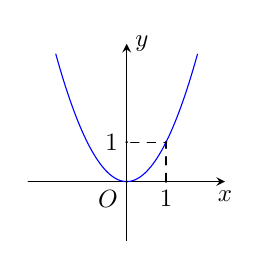
\begin{tikzpicture}[line join = round,line cap = round,>=stealth,scale=0.5]
		\draw[->]  (-2.5,0)--(0,0) node[below left]{$O$}--(2.5,0) node[below]{$x$};
		\draw[->] (0,-1.5)--(0,3.5) node[right]{$y$}; 
		\draw[samples=200,domain=-1.8:1.8,smooth,blue]  plot (\x,{(\x)^2}) node[below right]{$ $};
		 \draw[dashed](1,0)--(1,1)--(0,1);
		\node[below]  at (1,0){${1}$};
		 \node[left] at (0,1){${1}$};
		\fill (1,0) circle  (1pt);
		 \fill (0,1) circle (1pt);
		 \fill (1,1) circle (1pt);
		\fill (0,0) circle (1pt); 
	\end{tikzpicture}
		} 
		{ 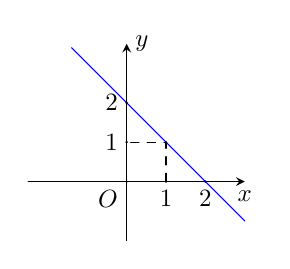
\begin{tikzpicture}[line join = round,line cap = round,>=stealth,scale=0.5]
		\draw[->] (-2.5,0)--(0,0) node[below left]{$O$}--(3,0)  node[below]{$x$};
		\draw[->] (0,-1.5)--(0,3.5) node[right]{$y$}; 
		\draw[samples=200,domain=-1.4:3,smooth,blue] plot (\x,{2-(\x)})  node[below right]{$ $};
		 \draw[dashed](1,0)--(1,1)--(0,1);
		\node[below]  at (1,0){${1}$};
		\node[below]  at (2,0){${2}$};
		\node[left] at  (0,1){${1}$};
		\node[left] at  (0,2){${2}$};
		\fill (1,0) circle (1pt); 
		\fill (0,1)  circle (1pt);
		\fill (1,1)  circle (1pt);
		 \fill (0,0) circle (1pt);
		\fill (0,2)  circle (1pt);
		\fill (2,0) circle (1pt); 
	\end{tikzpicture}
		 }
		{\True 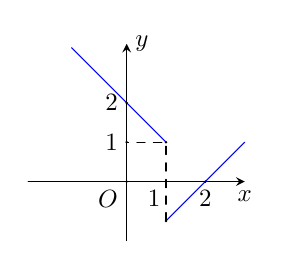
\begin{tikzpicture}[line join = round,line cap = round,>=stealth,scale=0.5]
		 \draw[->] (-2.5,0)--(0,0) node[below left]{$O$}--(3,0) node[below]{$x$};
		\draw[->] (0,-1.5)--(0,3.5) node[right]{$y$}; 
		\draw[samples=200,domain=-1.4:1,smooth,blue] plot (\x,{2-(\x)}) node[below right,blue]{$  $};
		\draw[samples=200,domain=1:3,smooth,blue] plot (\x,{-2+(\x)}) node[below right]{$ $}; 
		\draw[dashed](1,-1)--(1,1)--(0,1); 
		\node[below]  at (0.7,0){${1}$};
		\node[below] at (2,0){${2}$}; 
		 \node[left] at (0,1){${1}$};
		\node[left] at (0,2){${2}$}; 
		\fill (1,0) circle (1pt); 
		\fill (0,1)  circle (1pt);
		\fill (1,1) circle  (1pt);
		 \fill (0,0) circle (1pt);
		\fill  (0,2) circle (1pt);
		\fill  (2,0) circle (1pt);
		\fill (1,-1) circle  (1pt);
	\end{tikzpicture}
		 }
	 \loigiai{
		Đồ thị bị \lq\lq đứt\rq\rq\, tại điểm có hoành độ $x=1$ nên  nó không liên tục tại $x=1$.
	} 
\end{ex}

% từ: cau-hoi/lop11/1D3_Gioi_han_Ham_so_lien_tuc/1D3-3-4_Ham_so_lien_tuc_tren_khoang_doan.tex
\begin{ex}%[1D3K3-4]%[ma:b7c6b891]
	Cho $a;b;c$ theo thứ tự lập thành cấp  số cộng. Mệnh đề nào sau đây đúng?
	\choice 
		 { \True $a^2+{{c}^2}+2ac=4b^2$}
		{  $a^2+{{c}^2}=2ab-2bc$}
		{ $a^2-{{c}^2}=2ab-2bc$} 
		{  $a^2-{{c}^2}=ab-bc$}
	\loigiai{ 
	Ta có $a+c=2b\Rightarrow  {{(a+c)}^2}=4b^2\Leftrightarrow a^2+{{c}^2}+2ac=4b^2$.}
\end{ex}

% từ: cau-hoi/lop11/1D3_Gioi_han_Ham_so_lien_tuc/1D3-3-5_Bai_toan_phuong_trinh_co_nghiem.tex
\begin{ex}%[1D3H3-5]%[ma:792fe683]
	Cho phương trình $2x^3-8x-1=0 \quad (1)$. Khẳng định nào  sai?
	\choice 
		 {Phương trình $(1)$ không có nghiệm lớn hơn $3$}
		{Phương trình $(1)$ có đúng $3$ nghiệm phân biệt} 
		{\True Phương trình $(1)$ có  $2$ nghiệm lớn hơn $2$}
		{Phương trình $(1)$ có nghiệm trong khoảng $(-5; -1)$} 
	 \loigiai{
		Xét hàm số $f(x) =  2x^3 - 8x - 1$ liên tục trên $\mathbb{R}$.\\
		Do đó, hàm số liên tục trên các khoảng $(-5; -1)$, $(-1; 2)$,  và $(2; 3)$.\\
		 Ta có
		 \[
		\heva{ 
		 &f(-5) = -211 \\
		 &f(-1) = 5
		} \Rightarrow  f(-5) \cdot f(-1) < 0.
		\] 
		Suy ra phương trình $f(x) = 0$ có  ít nhất một nghiệm thuộc $(-5; -1)$.
		 \[
		 \heva{
		&f(-1) = 5 \\ 
		&f(2) = -1 
		} \Rightarrow  f(-1) \cdot f(2) < 0.
		 \]
		Suy ra phương trình $f(x)  = 0$ có ít nhất một nghiệm thuộc $(-1; 2)$.
		 \[
		 \heva{
		 &f(2) = -1 \\
		 &f(3) = 29
		} \Rightarrow f(2) \cdot f(3) <  0.
		\] 
		Suy  ra phương trình $f(x) = 0$ có ít nhất một nghiệm thuộc $(2; 3)$.\\
		Như vậy, phương trình $(1)$ có ít ba nghiệm phân biệt trên các khoảng $(-5; -1)$, $(-1;  2)$, và $(2; 3)$.\\
		Mà phương trình $(1)$ là phương trình bậc ba nên phương trình $(1)$ có đúng  ba nghiệm phân biệt trên các khoảng $(-5; -1)$, $(-1; 2)$, và $(2; 3)$.\\
		Vì vậy,  phương trình $(1)$ có đúng $1$ nghiệm lớn hơn $2$.
	 }
\end{ex}

% từ: cau-hoi/lop11/1D3_Gioi_han_Ham_so_lien_tuc/1D3-3-5_Bai_toan_phuong_trinh_co_nghiem.tex
\begin{ex}%[1D3V3-5]%[ma:efb8893c]
	Chứng minh rằng phương trình $6x^3+3x^2-31x+10=0$ có đúng  ba nghiệm phân biệt.
	 \loigiai{
		Đặt  $f(x)=6x^3+3x^2-31x+10$.\\
		 Tập xác định: $\mathscr{D}=\mathbb{R}$.\\
		$\Rightarrow f(x)$ liên tục trên $\mathbb{R} \Rightarrow f(x)$ liên tục  trên $[-3; 2]$.\\
		$\heva{&f(-3)=-32\\ &f(0)=10} \Rightarrow f(-3) \cdot  f(0) < 0\Rightarrow f(x)=0$ có nghiệm thuộc $(-3; 0)$.\\
		$\heva{&f(0)=10\\ &f(1)=-12} \Rightarrow f(0) \cdot f(1) <  0\Rightarrow f(x)=0$ có nghiệm thuộc $(1; 2)$.\\
		$\heva{&f(1)=-12\\ &f(2)=8}  \Rightarrow f(1) \cdot f(2) < 0\Rightarrow f(x)=0$ có nghiệm thuộc $(1; 2)$.\\
		Mặt khác vì $f(x)$ là một đa thức bậc ba nên $f(x)=0$ chỉ có tối đa ba nghiệm.\\ 
		Vậy phương trình $f(x)=0$  có đúng $3$ nghiệm phân biệt.
	 }
\end{ex}

% từ: cau-hoi/lop11/1D5_Cac_so_dac_trung_do_xu_the_trung_tam_cho/1D5-1-1_Cau_hoi_ly_thuyet.tex
\begin{ex}%[1D5Y1-1]%[ma:a43ea2ac]
	 Khẳng định nào sau đây là đúng?
	\choice 
		{\True $ f'(x_0)=\displaystyle  \lim_{x\to x_0}{\dfrac{f(x)-f(x_0)}{x-x_0}}
		 $}
		{$ f'(x_0)=\displaystyle  \lim_{x\to x_0}{\dfrac{f(x)+f(x_0)}{x-x_0}}
		$  }
		{$  f'(x_0)=\displaystyle \lim_{x\to x_0}{\dfrac{f(x_0)-f(x)}{x-x_0}}
		 $ }
		{$ f'(x_0)=\displaystyle \lim_{x\to  0}{\dfrac{f(x)-f(x_0)}{x-x_0}}
		$  }
	 \loigiai{
	 }
\end{ex}

% từ: cau-hoi/lop11/1D5_Cac_so_dac_trung_do_xu_the_trung_tam_cho/1D5-2-1_Cau_hoi_ly_thuyet.tex
\begin{ex}%[1D5B2-1]%[ma:a16c5396]
	Cho hàm số $f(x)=(2 x-1)^3$. Giá trị của $f"(1)$  bằng
	\choice 
		{$12$} 
		{$6$} 
		{\True  $24$}
		 {$4$}
	 \loigiai{
		 Ta có \\
		$\bullet\,\, f'(x)=3\cdot  (2 x-1)^2\cdot (2x-1)'=6 (2 x-1)^2$.\\
		 $\bullet\,\, f"(x)=12 (2x-1)(2x-1)'=24 (2x-1).$\\
		Vậy $f"(1)=24  (2\cdot 1-1)=24.$
	} 
\end{ex}

% từ: cau-hoi/lop11/1D5_Cac_so_dac_trung_do_xu_the_trung_tam_cho/1D5-2-1_Cau_hoi_ly_thuyet.tex
\begin{ex}%[1D5Y2-1]%[ma:e80bb502]
	Cho  hàm số $f(x)=2x^{3}+1$. Giá trị $f'(-1)$ bằng:
	 \choice
		{\True  $6$}
		{$3$} 
		{$-2$} 
		 {$-6$}
	\loigiai{ 
		Ta có $f'(x) =  6x^2 \Rightarrow f'(-1) = 6$.
	 }
\end{ex}

% từ: cau-hoi/lop11/1D5_Cac_so_dac_trung_do_xu_the_trung_tam_cho/1D5-2-1_Cau_hoi_ly_thuyet.tex
\begin{ex}%[1D5Y2-1]%[ma:e527a723]
	Cho  hàm số $ f(x)=x^4-3x^2+5. $ Tính $ f'(2).$
	 \choice
		{$ 4  $}
		{$  5 $}
		{\True $ 20  $}
		{$ 0  $}
	\loigiai{ 
		 Ta có $ f'(x)=4x^3-6x\Rightarrow f'(2)=20. $
	} 
\end{ex}

% từ: cau-hoi/lop11/1D5_Cac_so_dac_trung_do_xu_the_trung_tam_cho/1D5-2-1_Cau_hoi_ly_thuyet.tex
\begin{ex}%[1D5Y2-1]%[ma:aa6207f6]
	Cho hàm số $y=\cos 2x$. Công thức nào sau đây là  đúng?
	\choice 
		 {$y'=-\sin 2x$}
		{\True  $y'=-2\sin 2x$}
		{$y'=\sin 2x$} 
		{$y'=2\sin  2x$}
	 \loigiai{
		Ta có  $y'=(\cos 2x)'=-(2x)'\sin 2x=-2\sin 2x$.
	 }
\end{ex}

% từ: cau-hoi/lop11/1D6_Ham_so_mu_va_ham_so_logarit/1D6-1-3_Dieu_kien_cho_luy_thua_can_thuc.tex
\begin{ex}%[1D6H1-3]%[ma:9125bec1]
	 Tập xác định $\mathscr{D}$ của hàm số $y=\left(x^2-x-2\right)^{-3}$ là
	 \choice
		{$\mathscr{D}=\mathbb{R}$} 
		 {$\mathscr{D}=(-\infty;-1) \cup(2;+\infty)$}
		{$\mathscr{D}=(0;+\infty)$} 
		{\True $\mathscr{D}=\mathbb{R} \setminus\{-1;  2\}$}
	 \loigiai{
		Vì $-3$ là số nguyên âm nên hàm  số $y=\left(x^2-x-2\right)^{-3}$ xác định khi và chỉ khi
		$$x^2-x-2 \ne 0 \Leftrightarrow \heva{& x \ne -1 \\ &  x \ne 2.}$$
		Vậy tập xác định của hàm số là  $\mathscr{D}=\mathbb{R} \setminus\{-1; 2\}$.
	} 
\end{ex}

% từ: cau-hoi/lop11/1D6_Ham_so_mu_va_ham_so_logarit/1D6-2-2_Bien_doi_bieu_dien_bieu_thuc_chua_logarit.tex
\begin{ex}%[1D6V2-2]%[ma:288869cc]
	Ba số $a+\log _2 3$, $a+\log _4 3; a+\log _8 3$ theo thứ tự lập thành cấp số nhân. Công bội của cấp  số nhân này bằng
	 \choice
		 {$\dfrac{1}{4}$}
		{$1$} 
		 {\True $\dfrac{1}{3}$}
		{$\dfrac{1}{2}$} 
	\loigiai{Theo giả thiết,  ta có
		\allowdisplaybreaks 
		\begin{eqnarray*}
			\left(a+\log _4 3\right)^2=\left(a+\log _2 3\right)\left(a+\log _8 3\right) &\Leftrightarrow& a \log _2 3+\left(\dfrac{1}{2} \log  _2 3\right)^2=\dfrac{4}{3} a \log _2 3+\dfrac{1}{3}\left(\log _2 3\right)^2 \\&\Leftrightarrow& \dfrac{1}{3} a \log _2 3=-\dfrac{1}{12}\left(\log _2 3\right)^2 \\&\Leftrightarrow& a=-\dfrac{1}{4} \log _2 3.
		\end{eqnarray*}
		Vậy $q=\dfrac{a+\log _4 3}{a+\log _2 3}=\dfrac{-\dfrac{1}{4} \log  _2 3+\dfrac{1}{2} \log _2 3}{-\dfrac{1}{4} \log _2 3+\log _2 3}=\dfrac{1}{3}$.
	} 
\end{ex}

% từ: cau-hoi/lop11/1D6_Ham_so_mu_va_ham_so_logarit/1D6-4-2_Phuong_trinh_mu_logarit_co_ban.tex
\begin{bt}%[1D6H4-2]%[ma:5451ea73]
	Giải phương  trình sau $2^{x^2-x+8}=4^{1-3x}$.
	 \loigiai{
		\begin{eqnarray*}
			& &  2^{x^2-x+8}=4^{1-3x}\\
			 &\Leftrightarrow & 2^{x^2-x+8}=2^{2\left(1-3x\right)}\\
			& \Leftrightarrow & x^2-x+8=2-6x\\ 
			& \Leftrightarrow &  x^2+5x+6=0\\
			& \Leftrightarrow & \hoac{&x=-2\\&x=-3.} 
		\end{eqnarray*}
	 }
\end{bt}

% từ: cau-hoi/lop11/1D6_Ham_so_mu_va_ham_so_logarit/1D6-4-2_Phuong_trinh_mu_logarit_co_ban.tex
\begin{bt}%[1D6H4-2]%[ma:e66df748]
	Giải phương  trình: $2^x+2^{x+1}=4$.
	 \loigiai{
		 Ta có
		\begin{align*}
			& 2^x+2^{x+1}=4^x\\ 
			\Leftrightarrow\  &2^x+2\cdot 2^x=4\\
			\Leftrightarrow\ &2^x(1+2^1)=4\\ 
			\Leftrightarrow\ &2^x=\dfrac{4}{3}\\ 
			 \Leftrightarrow\ &x=\log_2\dfrac{4}{3}.
		\end{align*}
	} 
\end{bt}

% từ: cau-hoi/lop11/1D6_Ham_so_mu_va_ham_so_logarit/1D6-4-2_Phuong_trinh_mu_logarit_co_ban.tex
\begin{bt}%[1D6V4-2]%[ma:ef94fd43]
	Giải phương trình $2^x + 2^{x+1}  = 4$.
	 \loigiai{
		\begin{eqnarray*}
			&&2^x  + 2^{x+1} = 4\\
			&\Leftrightarrow&2^x + 2^x\cdot  2 = 4\\
			&\Leftrightarrow&3\cdot 2^x =  4\\
			&\Leftrightarrow&2^x = \dfrac{4}{3}\\ 
			 &\Leftrightarrow&x = \log_{2}\dfrac{4}{3}.
		\end{eqnarray*}
	} 
\end{bt}

% từ: cau-hoi/lop11/1D6_Ham_so_mu_va_ham_so_logarit/1D6-4-2_Phuong_trinh_mu_logarit_co_ban.tex
\begin{bt}%[1D6H4-2]%[ma:4f4f8c9e]
% nguon: Archive/SP_SauLuoi_2024-2025/Sp_GHKII/data/GHKII/1-TN-DS-TLN-TL-THPT-AnLuongDong-Hue-GHKII-NH24-25.tex #170
%[Dự án đề kiểm tra NH24-25 -đợt 9 - Nhật Thiện]%[THPT An Lương Đông - Huế]
	Giải phương trình $2^{x^2+6x-5}=4^x$.
	\loigiai{
	Ta có
	\begin{eqnarray*}
		& &2^{x^2+6x-5}=4^x\\
		&\Leftrightarrow& 2^{x^2+6x-5}=2^{2x}\\
		&\Leftrightarrow& x^2+6x-5=2x\\
		&\Leftrightarrow& \hoac{&x=1\\&x=-5.}
	\end{eqnarray*}
	Vậy tập nghiệm của phương trình là $S=\{1;-5\}$.
}
\end{bt}

% từ: cau-hoi/lop11/1D6_Ham_so_mu_va_ham_so_logarit/1D6-4-2_Phuong_trinh_mu_logarit_co_ban.tex
\begin{bt}%[1D6H4-2]%[ma:0bdae62b]
% nguon: Archive/SP_SauLuoi_2024-2025/Sp_GHKII/data/GHKII/1-TN-DS-TLN-TL-THPT-VinhLinh-QuangTri-GHKII-NH24-25.tex #291
%[Lớp 11 - Ôn tập giữa học kì 2 - THPT Vĩnh Linh-Quảng Trị]%[Trần Văn Hùng]
	Giải phương trình $5^{7x-3} = 25^{x+1}$.
	\loigiai{
Tập xác định $\mathscr{D}=\Bbb{R}$.\\
Ta có
\begin{eqnarray*}
&&5^{7x-3} = 25^{x+1}\\
&\Leftrightarrow& 5^{7x-3}=5^{2x+2}\\
&\Leftrightarrow& 7x-3=2x+2\\
&\Leftrightarrow& x=1.
\end{eqnarray*}
Vậy nghiệm của phương trình là $x=1$.
	}
\end{bt}

% từ: cau-hoi/lop11/1D6_Ham_so_mu_va_ham_so_logarit/1D6-4-2_Phuong_trinh_mu_logarit_co_ban.tex
\begin{bt}%[1D6N4-2]%[ma:11d308c3]
% nguon: Archive/SP-4Phan-Dot3/Data/CTST_1-OTHK2_De03.tex #4281

	Giải các phương trình sau $3^{x-1}=27$.
	\loigiai{
		Ta có $3^{x-1}=27\Leftrightarrow3^{x-1}=3^3\Leftrightarrow x-1=3\Leftrightarrow x=4$.
	}
\end{bt}

% từ: cau-hoi/lop11/1D6_Ham_so_mu_va_ham_so_logarit/1D6-4-4_Phuong_trinh_mu_logarit_dua_ve_cung_co_so.tex
\begin{ex}%[1D6V4-4]%[ma:240f5b79]
	Giải phương  trình $\sqrt{2^x\cdot\sqrt[3]{4^x}\cdot\sqrt[{3x}]{0{,}125}}=4\sqrt[3]2$.
	 \loigiai{
		Điều kiện $\heva{&x\ge \dfrac{1}{3} \\&3x\in  \mathbb{N}.}$\\
		Phương  trình đã cho tương đương với phương trình
		\begin{eqnarray*}
			\sqrt{2^x\cdot 2^{2\cdot \tfrac{x}{3}}\cdot \left(\dfrac{1}{8} \right)^{\tfrac{1}{3x}}}=2^2\cdot2^{\tfrac{1}{3}} &\Leftrightarrow& 2^{\tfrac{x}{2}}\cdot 2^{\tfrac{x}{3}}\cdot 2^{\tfrac{-1}{2x}}=2^{\tfrac{7}{3}}\\ 
			&\Leftrightarrow& 2^{\tfrac{x}{2}+\tfrac{x}{3}-\tfrac{1}{2x}}=2^{\tfrac{7}{3}}\\ &\Leftrightarrow& \dfrac{x}{2}+\dfrac{x}{3}-\dfrac{1}{2x}=\dfrac{7}{3}\\ &\Leftrightarrow&  5x^2-14x-3=0\\
			&\Leftrightarrow& \hoac{&x=-\dfrac{1}{5}\\&x=3.} 
		\end{eqnarray*}
		Kết hợp với điều  kiện ta có $x=3$ là nghiệm của phương trình.
	 }
\end{ex}

% từ: cau-hoi/lop11/1D6_Ham_so_mu_va_ham_so_logarit/1D6-4-4_Phuong_trinh_mu_logarit_dua_ve_cung_co_so.tex
\begin{bt}%[1D6H4-4]%[ma:25a478ed]
% nguon: Archive/SP_DA_SauLuoi/1-TL-THPT-NguyenThiMinhKhai-TpHCM-HKII-NH23-24.tex #2468
%[Dự án đề kiểm tra Toán 11 HKII NH23-24- Ngô Tất Thành]%[THPT Nguyễn Thị Minh Khai]
	Giải phương trình $2^{x^2+2x}=8^{2-x}$.
	\loigiai{
	Ta có $2^{x^2+2x}=8^{2-x} \Leftrightarrow 2^{x^2+2x}=2^{3(2-x)} \Leftrightarrow x^2+5x-6=0 \Leftrightarrow \hoac{&x=1\\ &x=-6.}$
	}
\end{bt}

% từ: cau-hoi/lop11/1D6_Ham_so_mu_va_ham_so_logarit/1D6-4-4_Phuong_trinh_mu_logarit_dua_ve_cung_co_so.tex
\begin{bt}%[1D6H4-4]%[ma:f212e272]
% nguon: Archive/SP_DA_SauLuoi/1-TL-THPT-NguyenTatThanh-HCM-HKII-NH23-24.tex #2551
%[Dự án đề kiểm tra Toán 11 HKII NH23-24- Trần Xuan Hòa]%[THPT NguyenTatTHanh]
Giải phương trình $5^{x^2-3 x}=25^{3-x}$.
	\loigiai{
Phương trình tương đương với $x^2-3 x=6-2 x \Leftrightarrow x^2-x-6=0 \Leftrightarrow \hoac{&x=3\\ &x=-2.}$\\
	Tập nghiệm là $S=\{-2;3\}$.
}
\end{bt}

% từ: cau-hoi/lop11/1D6_Ham_so_mu_va_ham_so_logarit/1D6-4-5_Bat_phuong_trinh_mu_logarit_dua_ve_cung_co_so.tex
\begin{bt}%[1D6H4-5]%[ma:287dbcbf]
	 Giải các bất phương trình sau
	\begin{listEX}[2]
		 \item $2^{2x-1}-2^{-2}>0$;
		\item $2^{2(x+5)^2}  \ge 4^{1-2x}$.
	\end{listEX}
	\loigiai{ 
		\begin{listEX}
			\item Ta có  $2^{2x-1}-2^{-2}>0 \Leftrightarrow 2^{2x-1}>2^{-2} \Leftrightarrow 2x-1>-2 \Leftrightarrow x>-\dfrac{1}{2}$.\\
			 Vậy tập nghiệm của bất phương trình là $S=\left(-\dfrac{1}{2};+\infty\right)$.
			\item Ta  có
			\begin{eqnarray*}
				 2^{2(x+5)^2} \ge 4^{1-2x}
				 &\Leftrightarrow& 4^{(x+5)^2} \ge 4^{1-2x}\\
				&\Leftrightarrow& (x+5)^2 \ge  1-2x \\
				&\Leftrightarrow& x^2+4x+24  \ge 0 \\
				&\Leftrightarrow& (x+2)^2+20>0, \  \forall x \in \mathbb{R}.
			\end{eqnarray*}
			Vậy tập nghiệm của bất phương trình là $S=\mathbb{R}$. 
		\end{listEX}
	} 
\end{bt}

% từ: cau-hoi/lop11/1D6_Ham_so_mu_va_ham_so_logarit/1D6-4-5_Bat_phuong_trinh_mu_logarit_dua_ve_cung_co_so.tex
\begin{bt}%[1D6H4-5]%[ma:6a00b715]
	Giải các bất phương  trình sau
	\begin{listEX}[2]
		 \item $2^{x+1}>8^{x-1}$;
		\item $3^{4^x} \le 4^{3^x}$. 
	\end{listEX}
	\loigiai{ 
		\begin{listEX}
			\item Ta có \begin{eqnarray*}
			2^{x+1}>8^{x-1} 
			&\Leftrightarrow&  x+1>(x-1)\log_2 8\\
			&\Leftrightarrow& x+1>3(x-1)\\ 
			 &\Leftrightarrow& x<-2.
		\end{eqnarray*}
		 Vậy tập nghiệm của bất phương trình là $S=\left(-\infty;-2\right)$.
		\item Ta có \begin{eqnarray*}
		 3^{4^x} \le 4^{3^x}
		&\Leftrightarrow& 4^x \log_3 3 \le  3^x \log_3 4\\
		&\Leftrightarrow& \left(\dfrac{4}{3}\right)^x \le \log_3 4\\ 
		 &\Leftrightarrow& x \le \log_{\tfrac{4}{3}}\left(\log_3 4\right).
	\end{eqnarray*}
	Vậy tập nghiệm của bất phương trình là $S=\left(-\infty;\log_{\tfrac{4}{3}}\left(\log_3  4\right)\right]$.
	\end{listEX}
 }
\end{bt}

% từ: cau-hoi/lop11/1D7_Dao_ham/1D7-2-6_Gioi_han_ham_so_luong_giac_ham_so_mu_logarit.tex
\begin{ex}%[1D7V2-6]%[ma:89effb5e]
	Cho hàm số $f(x)=\sin 2x+\sqrt{3}\cos 2x+12\sin \left(x+\dfrac{\pi}{6}\right)$. Họ nghiệm của phương trình $f'(x)+4=0$ có dạng  $x=\dfrac{\pi}{m}+k\pi$ với $m$ nguyên dương, $k\in \mathbb{Z}$. Giá trị của $m$ bằng
	 \shortans{3}
	\loigiai{ 
		\begin{itemize}
			\item $f'(x)=2\cos 2x-2\sqrt{3}\sin 2x+12\cos\left(x+\dfrac{\pi}{6}\right).$ 
			 \item $f'(x)+4=0\Leftrightarrow \dfrac{1}{2}\cos 2x-\dfrac{\sqrt{3}}{2}\sin 2x+3\cos \left(x+\dfrac{\pi}{6}\right)+1=0$\\
			$\Leftrightarrow \cos\left(2x+\dfrac{\pi}{3}\right)+3\cos\left(x+\dfrac{\pi}{6}\right)+1=0\Leftrightarrow 2\cos^2\left(x+\dfrac{\pi}{6}\right)+3\cos\left(x+\dfrac{\pi}{6}\right)=0$\\ 
			$\Leftrightarrow \cos\left(x+\dfrac{\pi}{6}\right)=0$ (vì  $\cos\left(x+\dfrac{\pi}{6}\right)\in [-1;1]$).\\
			$\Leftrightarrow x+\dfrac{\pi}{6}=\dfrac{\pi}{2}+k\pi\Leftrightarrow x=\dfrac{\pi}{3}+k\pi, k\in\mathbb{Z}$.\\ 
			 Vậy $m=3$.
		\end{itemize}
	 }
\end{ex}

% từ: cau-hoi/lop11/1D7_Dao_ham/1D7-2-8_Toan_thuc_te_ap_dung_quy_tac_dao_ham.tex
\begin{ex}%[1D7H2-8]%[ma:8ab67612]
	Một vật chuyển động trên đường thẳng được xác định bởi công thức $s(t)=t^3-3t^2+7t-2$, trong đó $t > 0$ và tính bằng giây, $s$ là quãng đường chuyển động được  của vật trong $t$ giây và được tính bằng mét.
	 \choiceTF
		{\True Sau $5$ giây, vật chuyển động  quãng đường là $83$\,m}
		{Vận tốc tức thời  của vật tại thời điểm $t=5$ là $50$\,m/s}
		{Khi vận tốc của chuyển động bằng $151$ $m/s$ thì quãng đường vật chuyển động được là $352$\,m} 
		{\True Tại thời điểm $t=1$ giây, vận  tốc của chuyển động đạt giá trị nhỏ nhất}
	\loigiai{ 
		\begin{itemchoice}
			\itemch Ta có  $s(5)=5^3-3\cdot 5^2+7\cdot 5-2=83$.\\
			Vậy  sau $5$ giây, vật chuyển động quãng đường là $83$\,m.
			\itemch Vì $v(t)=s'(t)=3t^2-6t+7$ nên $v(5)=3\cdot 5^2-6\cdot 5+7=52$\,(m/s). 
			\itemch Vận tốc của chuyển động bằng $151$ m/s tại thời điểm $t$ nghĩa là \[v(t)=151\Leftrightarrow 3t^2-6t+7=151\Leftrightarrow 3t^2-6t-144=0\Leftrightarrow \hoac{&t=-6&\text{ (loại)}\\&t=8.}\] 
			Quãng  đường vật chuyển động sau $8$ giây là $s(8)=8^3-3\cdot 8^2+7\cdot 8-2=374$\,(m).\\
			Vậy khi vận tốc của chuyển động bằng $151$ $m/s$ thì  quãng đường vật chuyển động được là $374$\,m.
			\itemch Vận tốc tức thời của chuyển động có phương trình $v(t)=3t^2-6t+7$ là  một parabol, có đỉnh $S\left(-\dfrac{b}{2a};-\dfrac{\Delta}{4a}\right)\Rightarrow S(1;4)$ và hệ số $a=3> 0$ nên hàm số có giá trị nhỏ nhất bằng $4$ tại $t=1$.\\
			Vậy tại thời điểm $t=1$ thì vận tốc của chuyển động đạt giá trị  nhỏ nhất bằng $4$\,m/s.
		\end{itemchoice}
	 }
\end{ex}

% từ: cau-hoi/lop11/1D7_Dao_ham/1D7-2-8_Toan_thuc_te_ap_dung_quy_tac_dao_ham.tex
\begin{ex}%[1D7H2-8]%[ma:3403ff36]
	Cho chuyển động thẳng xác định bởi phương trình $s=-t^3+3t^2+9t$, trong đó $t$ tính bằng giây và $s$ tính bằng mét.  Tính vận tốc của chuyển động tại thời điểm gia tốc triệt tiêu.
	\shortans{12} 
	\loigiai{ 
		Gia  tốc chuyển động tại $t=3$ là $ s''(3) $.\\
	Ta có $s'(t)=3t^2-6t+5$; $s''(t)=6t-6\Rightarrow s''(3)=12$ m/s$^2$.} 
\end{ex}

% từ: cau-hoi/lop11/1D7_Dao_ham/1D7-2-8_Toan_thuc_te_ap_dung_quy_tac_dao_ham.tex
\begin{ex}%[1D7V2-8]%[ma:56e755f0]
	Cho chuyển động thẳng xác định bởi phương trình $s(t)=-t^3+3t^2+9t$, trong đó $t$ tính bằng giây và $s$ tính bằng mét. Vận tốc của chuyển động tại thời điểm gia tốc triệt tiêu bằng bao  nhiêu?
	 \shortans{12}
	\loigiai{ 
		Vận  tốc của chuyển động chính là đạo hàm cấp một của quãng đường $$v(t)=s'(t)=-3t^2+6t+9.$$
		Gia tốc của chuyển động chính là đạo  hàm cấp hai của quãng đường $$a(t)=s''(t)=-6t+6.$$
		Gia tốc triệt  tiêu khi $s''(t)=0\Leftrightarrow t=1$.\\
	Khi đó vận tốc của chuyển động là  $s'(1)=12$ m/ s.}
\end{ex}

% từ: cau-hoi/lop11/1D7_Dao_ham/1D7-2-8_Toan_thuc_te_ap_dung_quy_tac_dao_ham.tex
\begin{bt}%[1D7V2-8]%[ma:61df70be]
% nguon: Archive/SP-4Phan-Dot3/Data/CD_1_OTHK2_De04.tex #4299

	Giả sử một chất điểm chuyển động trong $30$ giây đầu tiên có phương trình $s(t)=\dfrac{1}{12}t^4-t^3+6t^2+12t+2$, trong đó $t>0$ với $t$ tính bằng giây $(s)$ và $s(t)$ tính bằng mét (m). Tìm vận tốc của vật tại thời điểm gia tốc của vật đạt giá trị nhỏ nhất.
	\shortans[0]{$30$}
	\loigiai{
		Vận tốc chất điểm là $v(t)=s'(t)=\dfrac{1}{3}t^3-3t^2+12t+12$.\\
		Gia tốc của chất điểm là $a(t)=v'(t)=t^2-6t+12=(t-3)^2+3\ge 3$, $\forall t$.\\
		Gia tốc vật nhỏ nhất khi và chỉ khi $t=3$.\\
		Khi đó vận tốc là $v(3)=30$ (m/s).
	}
\end{bt}

% từ: cau-hoi/lop11/1D7_Dao_ham/1D7-3-1_Tinh_dao_ham_cap_hai.tex
\begin{ex}%[1D7H3-1]%[ma:69bb550a]
	Có bao nhiêu cặp số nguyên dương $(a; b)$ thỏa mãn $\log_{a}b+6 \log_{b} a=5$  và $a \in[2; 2005]$, $b \in[2;2005]$?
	 \shortans{54}
	 \loigiai{
		Với các điều kiện trên, ta có 
		\begin{eqnarray*}
			&&\log_{a}b+6 \log_{b} a=5 
			 \\
			&\Leftrightarrow& \log_a  b +6 \dfrac{1}{\log_a b}=5
			\\ 
			&\Leftrightarrow&  \log^2_a b -5\log_a b+6=0
			 \\
			&\Leftrightarrow& \hoac{& \log_a b  =2 \\ & \log_a b =3}
			 \\
			&\Leftrightarrow& \hoac{&  b=a^2 \\ & b=a^3.}
		\end{eqnarray*}
		Khi $b=a^2 \Rightarrow 2\le a^2 \le 2005 \Rightarrow \sqrt  2 \le a \le \sqrt{2005}$.
		\\ 
		Do $a$ nguyên nên $2\le a \le 44$, vậy có $44-2+1=43$ số $a$ thoả mãn nên có $43$  cặp số $a$, $b$ thoả mãn yêu cầu bài toán.
		 \\
		Khi $b=a^3 \Rightarrow 2\le a^3 \le 2005 \Rightarrow \sqrt[3] 2 \le a \le  \sqrt[3]{2005}$.
		 \\
		Do $a$ nguyên nên $2\le a \le 12$, vậy có $12-2+1=11$ số $a$ thoả mãn nên có $11$ cặp số $a$, $b$  thoả mãn yêu cầu bài toán.
		\\ 
		Vậy có tổng cộng $43+11=54$ cặp  số thoả mãn.
	 }
\end{ex}

% từ: cau-hoi/lop11/1D7_Dao_ham/1D7-3-1_Tinh_dao_ham_cap_hai.tex
\begin{ex}%[1D7H3-1]%[ma:171a4ab8]
	Cho  $f(x)=\sin 3x$. Tính $f''\left(-\dfrac{\pi}{2}\right)$, $f''(0)$, $f''\left(\dfrac{\pi}{18}\right)$.
	 \loigiai{
		 Ta có $f'(x)=3\cos 3x$ và $f''(x)=-9\sin 3x$.\\
		Khi đó 
		\begin{itemize}
			\item $f''\left(-\dfrac{\pi}{2}\right)=-9\sin\left(-\dfrac{3\pi}{2}\right)=-9$; 
			 \item $f''(0)=-9\sin (0)=0$;
			\item  $f''\left(\dfrac{\pi}{18}\right)=-9\sin\left(\dfrac{\pi}{6}\right)=\dfrac{-9}{2}$.
		\end{itemize}
	 }
\end{ex}

% từ: cau-hoi/lop11/1H8_Quan_he_vuong_goc_trong_khong_gian/1H8-1-3_Tim_goc_giua_hai_duong_thang.tex
\begin{bt}%[1H8V1-3]%[ma:86ec9cc0]
	Cho hình chóp $S. A B C D$ có đáy là hình bình hành tâm $O$. Biết $\widehat{S A D}=\widehat{S C  D}=90^{\circ}$. Tìm số đo của góc $(S B, A C)$
	\loigiai{ 
	\immini{ 
		Gọi  $M$ là trung điểm cạnh $S D$.\\
		Khi đó $O M$ là đường trung bình của tam giác $S B D$ nên $O M \parallel  S B$.\\
		Do vậy $(S  B, A C)=(O M, A C)$.\\
		Tam giác $S A  D$ vuông tại $A$ có trung tuyến $A M=\dfrac{S D}{2}$;\\
		Tam giác $S C D$ vuông tại $C$  có trung tuyến $C M=\dfrac{S D}{2}$.\\
		Suy ra tam giác $M  A C$ cân tại $M$, mà $O$ là trung điểm $A C$ nên $O M \perp A C$ hay $(O M, A C)=90^{\circ}$. Do đó $(S B, A C)=90^{\circ}$ hay $S B \perp A C$.
		} 
		{ 
		\begin{tikzpicture}[scale=0.9]
				 \tkzDefPoints{0/0/D,-2/-2/C,2.5/-2/B}
				\coordinate (A)  at ($(B)+(D)-(C)$);
				\draw (C)--(B)--(A); 
				 \draw[dashed] (C)--(D)--(A);
				\coordinate (O) at ($(A)!0.5!(C)$); 
				\coordinate (S)  at ($(O)+(-0.5,5)$);
				\coordinate  (M) at ($(S)!0.5!(A)$);
				\draw[dashed] (O)--(S)--(D)--(B) 
					 (A)--(C)
					(D)--(M)--(O); 
				\draw (S)--(A) 
					(S)--(B)--(M) 
					 (S)--(C);
				\tkzMarkRightAngle  (A,O,D)
				 \tkzMarkRightAngle (S,D,A)
				\tkzMarkRightAngle (S,B,A) 
				\begin{footnotesize}
					\draw (S) node[above]{$S$}; 
					 \draw (C) node[left]{$B$};
					 \draw (D) node[left]{$A$};
					\draw (A) node[right]{$D$}; 
					\draw  (B) node[right]{$C$};
					\draw  (M) node[right]{$M$};
					\draw  (O) node[below]{$O$};
				\end{footnotesize}
			\end{tikzpicture}
		} 
	} 
\end{bt}

% từ: cau-hoi/lop11/1H8_Quan_he_vuong_goc_trong_khong_gian/1H8-2-3_Xac_dinh_hoac_chung_minh_hai_duong_thang_vuon.tex
\begin{ex}%[1H8H2-3]%[ma:aea7229a]
	Cho hình lập phương $ABCD.A'B'C'D'$ có cạnh bằng $a$. Gọi $M$, $N$  lần lượt là trung điểm của $A'B'$, $B'C'$. Góc giữa hai đường thẳng $MN$ và $BD$ là (đơn vị độ)
	 \shortans{90}
	\loigiai{ 
	 \immini{
		 Ta có $MN\parallel AC$ mà $AC\perp BD\Rightarrow MN\perp BD$.\\
		Vậy $(MN,BD)=90^\circ$. 
		}{ 
		\begin{tikzpicture}[line cap=round,line join=round,>=stealth,>=latex,font=\footnotesize,scale=.75]
				\def\h{4} 
				 \path
					(0,0) coordinate (A') 
					(4,0) coordinate  (D')
					(-2,-1) coordinate  (B')
					($(B')+(D')-(A')$) coordinate (C') 
					($(A')+(90:\h)$) coordinate (A) 
					($(B')+(90:\h)$) coordinate (B) 
					($(C')+(90:\h)$) coordinate (C) 
					($(D')+(90:\h)$) coordinate  (D)
					($(B')!.5!(A')$)  coordinate (M)
					($(B')!.5!(C')$) coordinate (N); 
				 \draw (A)--(B)--(C)--(D)--cycle (B)--(B')--(C')--(C)
					 (C')--(D')--(D)
					 (B)--(D)
					 (A)--(C);
				\draw[dashed] (A)--(A') 
					 (B')--(A')--(D')
					 (M)--(N);
				\foreach \x/\g in {A/90,B/180,C/-45,D/0,A'/135,B'/180,C'/-45,D'/0,M/135,N/-90} 
				\fill  (\x) circle (1pt)
					($(\g:3mm)+(\x)$) node  {$\x$};
			\end{tikzpicture}
		 }
	} 
\end{ex}

% từ: cau-hoi/lop12/2D1_Ung_dung_dao_ham_de_khao_sat_ham_so/2D1-1-1_Xet_tinh_don_dieu_cua_ham_so_cho_boi_cong_thu.tex
\begin{ex}%[2D1N1-1]%[ma:3410019a]
	Hàm số $y = \dfrac{2x+3}{x+1}$ có bao  nhiêu điểm cực trị?
	 \choice
		 {$3$}
		 {$2$}
		{\True  $0$}
		 {$1$}
	 \loigiai{
		Tập xác định $\mathscr{D}  = \mathbb{R} \setminus \{-1\}$. Đạo hàm $y'=\dfrac{-1}{(x+1)^2} <0$, $\forall x \neq -1$.\\
		Khi đó hàm  số luôn nghịch biến trên từng khoảng xác định.\\
		Vậy hàm số đã cho không  có cực trị.
	 }
\end{ex}

% từ: cau-hoi/lop12/2D1_Ung_dung_dao_ham_de_khao_sat_ham_so/2D1-1-2_Xet_tinh_don_dieu_dua_vao_bang_bien_thien_do.tex
\begin{ex}%[2D1H1-2]%[ma:58fb6c56]
	Cho hàm số $y=f(x)$ xác định và liên tục trên $\mathbb{R}$,  đồ thị của hàm số $y=f'(x)$ như hình vẽ.
	\begin{center}
		\begin{tikzpicture}[scale=1,font=\footnotesize,line join=round,line cap=round,>=stealth]
			 \draw[->] (-1.5,0)--(3,0) node[below] {$x$};
			\draw[->] (0,-1)--(0,3) node[left]  {$y$};
			\draw (0,0) node  [below left] {$O$};
			\fill (-1,0)  circle (1pt) node[above left] {$-1$}
				(1,0) circle (1pt) node[below left]  {$1$}
				(2,0) circle (1pt)  node[below right] {$2$};
			 \draw[smooth,samples=200] plot[domain=-1.15:2.55] (\x,{(\x)^3-2*(\x)^2-(\x)+2});
		\end{tikzpicture}
	\end{center}
	Kết luận nào sau đây là  đúng?
	\choice 
		{\True $f(3)<f(4)$} 
		{$f(-2)<f(-1)$} 
		{$f(3)>f(4)$} 
		{$f'(0)=0$} 
	\loigiai{ 
		 Trong khoảng $(2;+\infty)$ hàm số đồng biến, các giá trị $x$ bằng $3$; $4$ thuộc khoảng $(2;+\infty)$.\\
		Suy  ra $f(3)<f(4)$.
	 }
\end{ex}

% từ: cau-hoi/lop12/2D1_Ung_dung_dao_ham_de_khao_sat_ham_so/2D1-1-3_Tim_tham_so_de_ham_so_don_dieu.tex
\begin{bt}%[2D1V1-3]%[ma:03fb24d5]
	Đồ thị hàm số $y=x^3-3x^2+2ax+b$ có điểm cực tiểu $A(2;-2)$. Khi đó $a+b$ bằng bao  nhiêu?
	 \shortans{2}
	\loigiai{ 
		Ta có $y=x^3-3x^2+2ax+b$ xác  định trên $\mathbb{R}$, $y'=3x^2-6x+2a$.\\
		Vì đồ thị hàm số có  điểm cực tiểu $A(2;-2)$ nên ta có
		$\heva{&y(2)=-2\\&y'(2)=0}\Leftrightarrow\heva{&-4a+b=2 \\ &a=0} \Rightarrow \heva{&a=0 \\  &b=2.}$\\
		Suy ra hàm số $y=x^3-3x^2+2$.\\ 
		Thử lại ta thấy điểm $A(2;-2)$ là điểm cực tiểu của đồ thị  hàm số $y=x^3-3x^2+2$.\\
		 Vậy $a+b=2$.
	 }
\end{bt}

% từ: cau-hoi/lop12/2D1_Ung_dung_dao_ham_de_khao_sat_ham_so/2D1-1-4_Ung_dung_tinh_don_dieu_de_chung_minh_bat_dang.tex
\begin{bt}%[2D1V1-4]%[ma:fa37fc09]
% nguon: Archive/2024/TaiLieuGiangDay/1.HamSo/1. K12 - 4in1 - Hamso/Thubai/Bai1-Dang4_converted_converted.tex #2965
%%[Mức độ 3]%[Dự án bài giảng new 4in1, Trần Quang Thạnh]
Giải bất phương trình $ \log_2(2^x+1)+\log_3(4^x+2)\le 2$.\hfill $ (*) $
\loigiai{
\begin{itemize}
\item Điều kiện $ \begin{cases}2^x+1 > 0\\4^x+2 > 0\end{cases} $ đúng $ \forall x\in \mathbb{R}\Rightarrow $ Tập xác định $ \mathscr{D}=\mathbb{R} $.
\item Xét hàm số $ f(x)=\log_2(2^x+1)+\log_3(4^x+2) $ trên $ \mathbb{R} $.\\
Ta có $ f'(x)=\dfrac{2^x\ln2}{(2^x+1)\ln2}+\dfrac{4^x\ln4}{(4^x+1)\ln3} > 0,\forall x\in \mathbb{R}\Rightarrow $ Hàm số $ y=f(x) $ luôn đồng biến trên $ \mathbb{R} $.\\
Ta có $ f(0)=2 $ do đó $ \forall x\le 0 $ thì $ f(x)\le f(0)\Leftrightarrow x\le0 $.
\item Vậy tập nghiệm của bất phương trình là $ x\in (-\infty;0] $.
\end{itemize}}
\end{bt}

% từ: cau-hoi/lop12/2D1_Ung_dung_dao_ham_de_khao_sat_ham_so/2D1-1-5_Toan_thuc_te_ung_dung_su_dong_bien_nghich_bie.tex
\begin{bt}%[2D1H1-5]%[ma:f276548b]
	\immini{Một vật  chuyển động. Quãng đường $s(t)$ (tính theo mét) vật đi được sau khoảng thời gian $t$ (tính theo giây), $t \geq 0$, được mô tả là một hàm số bậc ba có đồ thị như hình vẽ dưới đây.
	Hỏi trong $10$  giây đầu tiên, khoảng thời gian vật chuyển động nhanh dần kéo dài bao~nhiêu giây?
	}{\resizebox{!}{5cm}{ 
	\begin{tikzpicture}[line join=round,line cap=round,>=stealth]
		 \def\xmin{-1}\def\xmax{5.8}\def\ymin{-1}\def\ymax{9}
		 \draw[->] (\xmin-0.2,0)--(\xmax+0.2,0) node[below] {$t (s)$};
		\draw[->]  (0,\ymin-0.2)--(0,\ymax+0.2) node[right] {$s (t)$(m)};
		\draw (0,0)  node [below left] {$O$};
		 \foreach \x in {2,4,5}\fill (\x,0) circle (1pt);
		\foreach \y in  {1.33,2.66,5.83}\fill (0,\y) circle (1pt);
		\clip (\xmin,\ymin) rectangle (\xmax,\ymax); 
		 \draw[smooth,samples=100,domain=0:\xmax] plot (\x,{(1/6)*((\x)^3)+-1*((\x)^2)+2*(\x)+0});
		\draw[dashed] (0,1.33)--(2,1.33)--(2,0) node[below]{$4$}; \fill (2,1.33) circle  (1pt);
		\fill  (0,1.33) circle (1pt) node [left] {$\dfrac{8}{3}$};
		\draw[dashed]  (0,2.66)--(4,2.66)--(4,0) node[below]{$8$};
		\fill  (4,2.66) circle (1pt);
		\fill (0,2.66) circle (1pt) node [left]  {$\dfrac{112}{3}$};
		 \draw[dashed] (0,5.83)--(5,5.83)--(5,0) node[below]{$10$};
		 \fill (5,5.83) circle (1pt);
		\fill (0,5.83) circle (1pt) node [left]  {$\dfrac{260}{3}$};
	\end{tikzpicture}
	}} 
	 \shortans{8}
	 \loigiai{
		 Gọi $s(t)=at^3+bt^2+ct+d$ $a\neq0$.\\
		Vì đồ thị hàm số $s(t)$ đi qua các điểm $(0;0)$, $\left( 4;\dfrac{8}{3} \right)$, $\left( 8;\dfrac{112}{3} \right)$,  $\left( 10;\dfrac{260}{3} \right)$.\\
		Nên ta có 
		$$\heva{&64a+16b+4c=\dfrac{8}{3} \\&512a+64b+8c=\dfrac{112}{3} \\&1000a+100b+10c=\dfrac{260}{3} \\&d=0} \Leftrightarrow  \heva{&a=\dfrac{1}{6} \\&b=-1 \\&c=2 \\&d=0.}$$
		Do đó $s(t)=\dfrac{1}{6}t^3-t^2+2t  \Rightarrow v(t)=s'(t)=\dfrac{1}{2}t^2-2t+2$.\\
		 Xét $v'(t)=0 \Leftrightarrow t=2$.\\
		 Bảng biến thiên
		\begin{center}
			
\begin{tikzpicture}
				\tkzTabInit[nocadre,lgt=1.2,espcl=2.5,deltacl=0.6] 
					 {$t$/0.6,$v'$/0.6,$v$/2}{$0$,$2$,$10$}
				\tkzTabLine{,-,0,+,} 
				 \tkzTabVar{+/$2$,-/$0$,+/$32$}
			\end{tikzpicture}
		\end{center}
		Dựa vào bảng biến thiên, từ giây thứ $2$ trở đi vận tốc của vật tăng  dần theo thời gian.\\
		Do đó trong $10$ giây đầu tiên, khoảng thời gian vật chuyển  động nhanh dần kéo dài trong $8$ giây.
	} 
\end{bt}

% từ: cau-hoi/lop12/2D1_Ung_dung_dao_ham_de_khao_sat_ham_so/2D1-1-5_Toan_thuc_te_ung_dung_su_dong_bien_nghich_bie.tex
\begin{bt}%[2D1V1-5]%[ma:9fb4ff77]
	Hàm số $y=\sqrt{1-x}+\sqrt{x+2}$ có tập xác định là  $\mathscr{D}=\left[a;b\right]$. Tính $a+2b$.
	 \shortans{0}
	 \loigiai{
		Hàm số  $y=\sqrt{1-x}+\sqrt{x+2}$ xác định khi
		 $\heva{&1-x\ge 0 \\&x+2\ge 0}\Leftrightarrow \heva{&x\le 1 \\&x\ge -2}
		 \Leftrightarrow -2\le x\le 1$.\\
		 Hay tập xác định của hàm số đã cho là $\mathscr{D}=[-2; 1]$.\\
		Do đó $a=-2$,  $b=1$.\\ Vậy $a+2b=0$.
	} 
\end{bt}

% từ: cau-hoi/lop12/2D1_Ung_dung_dao_ham_de_khao_sat_ham_so/2D1-2-1_Tim_cuc_tri_cua_ham_so_cho_boi_cong_thuc.tex
\begin{bt}%[NBV2526]%[2D1V2-1]%[ma:476c7691]
	Một vật chuyển động với vận tốc (m/s) được xác định bởi hàm số $f(t) = -t^3 + 3t^2$ với $t \geq 0$. Khi đó $f'(t)$ là gia tốc của vật tại thời điểm $t$ (giây). Vận tốc của vật đạt được cao nhất trong khoảng thời gian $3$ giây đầu là  bao nhiêu m/s?
	 \shortans{4}
	\loigiai{ 
		Ta có:  $f'(t) = -3t^2 + 6t$.\\
		Giải $f'(t)=0 \Leftrightarrow  \hoac{&t=2\\&t=0.}$\\
		Ta có bảng  biến thiên
		\begin{center}
			
\begin{tikzpicture}[>=stealth,scale=1]
				\tkzTabInit[lgt=1.5,espcl=3] 
					{$t$ /.7,$f'(t)$ /.7,$f  (t)$ /1.8}
					{$0$,$2$,$3$} 
				 \tkzTabLine{,+,$0$,-,}
				\tkzTabVar{-/,+/$4$,-/} 
			\end{tikzpicture}
		\end{center}
		Vận tốc của vật đạt cao nhất là  $4$ m/s.
	 }
\end{bt}

% từ: cau-hoi/lop12/2D1_Ung_dung_dao_ham_de_khao_sat_ham_so/2D1-3-1_GTLN_GTNN_tren_doan.tex
\begin{ex}%[2D1N3-1]%[ma:ef733eb4]
	 Cho $ac\neq 0$, $ad-bc\neq 0$. Đồ thị hàm số $y=\dfrac{ax+b}{cx+d}$ có đường tiệm cận đứng là
	 \choice
		{$x=\dfrac{a}{c}$} 
		{\True  $x=\dfrac{-d}{c}$}
		 {$y=\dfrac{a}{c}$}
		 {$y=\dfrac{-d}{c}$}
	 \loigiai{
		Đồ thị hàm số có tiệm  cận đứng là $x=-\dfrac{d}{c}$.
	 }
\end{ex}

% từ: cau-hoi/lop12/2D1_Ung_dung_dao_ham_de_khao_sat_ham_so/2D1-3-1_GTLN_GTNN_tren_doan.tex
\begin{ex}%[2D1N3-1]%[ma:30d94805]
	Cho $acd\neq 0$. Đồ thị hàm số $y=ax+b+\dfrac{c}{dx+e}$ ($a$, $b$,  $c$, $d$, $e\in\mathbb{R})$ có đường tiệm cận xiên là
	\choice 
		{\True  $y=ax+b$}
		{$y=dx+c$} 
		{$y=bx+a$} 
		 {$y=ex+d$}
	 \loigiai{
		Vì $\lim\limits_{x \to \pm \infty} [y-(ax+b)]=\lim\limits_{x \to \pm \infty} \dfrac{c}{dx + e}=0$ nên đồ  thị hàm số có tiệm cận xiên là $y = ax + b$.
	} 
\end{ex}

% từ: cau-hoi/lop12/2D1_Ung_dung_dao_ham_de_khao_sat_ham_so/2D1-3-1_GTLN_GTNN_tren_doan.tex
\begin{ex}%[2D1H3-1]%[ma:ca935c5a]
	Cho hàm số  $f(x) = \sin2x - x$.
	 \choiceTF
		 {$f\left(-\dfrac{\pi}{2}\right) = \dfrac{\pi}{2}, \quad f\left(\dfrac{\pi}{2}\right) = -\dfrac{\pi}{2}
		$} 
		{\True Đạo hàm  của hàm số là~$y'=\cos 2x-1$}
		{Nghiệm của phương trình $f'(x) = 0$ trên  đoạn $\left[-\dfrac{\pi}{2}; \dfrac{\pi}{2}\right]$ phương trình có nghiệm là~$x = -\dfrac{\pi}{6}; x = \dfrac{\pi}{6}$}
		{\True Giá trị nhỏ nhất của $f(x)$  trên đoạn $\left[-\dfrac{\pi}{2}; \dfrac{\pi}{2}\right]$ là~$f(x) = -\dfrac{\pi}{2}$}
	\loigiai{\begin{itemchoice}
		 \itemch \textbf{Đúng}.\\
		$f\left(-\dfrac{\pi}{2}\right) =  \sin(-\pi) - \left(-\dfrac{\pi}{2}\right) = \sin(-\pi) + \dfrac{\pi}{2} = \sin\pi + \dfrac{\pi}{2} = \dfrac{\pi}{2}
		$. 
		 \itemch \textbf{Sai}.\\
		Đạo hàm của hàm số  $f'(x) = 2\cos(2x) - 1$.
		\itemch  \textbf{Đúng}.\\
		 $f'(x) = 2\cos(2x) - 1 = 0$\\
		$  \Leftrightarrow \cos(2x) = \dfrac{1}{2}$\\
		$\Leftrightarrow x = -\dfrac{\pi}{6}$; $x = \dfrac{\pi}{6}$ là~nghiệm trên đoạn $\left[-\dfrac{\pi}{2}; \dfrac{\pi}{2}\right]$. 
		 \itemch \textbf{Đúng}.\\
		Nghiệm $x = \pm\dfrac{\pi}{6}$ thuộc  đoạn $\left[-\dfrac{\pi}{2}; \dfrac{\pi}{2}\right]$.
		\[ 
		f\left(-\dfrac{\pi}{2}\right) = \dfrac{\pi}{2}, \quad f\left(\frac{\pi}{2}\right)  = -\dfrac{\pi}{2}, \quad f\left(\dfrac{\pi}{6}\right) = \dfrac{\sqrt{3}}{2}-\dfrac{\pi}{6}
		, \quad f\left(-\dfrac{\pi}{6}\right) = -\dfrac{\sqrt{3}}{2}  + \dfrac{\pi}{6}.
		\] 
		Giá trị nhỏ nhất  là~$-\dfrac{\pi}{2}$.
	\end{itemchoice}
 }
\end{ex}

% từ: cau-hoi/lop12/2D1_Ung_dung_dao_ham_de_khao_sat_ham_so/2D1-5-4_Su_tuong_giao_cua_hai_do_thi_lien_quan_den_to.tex
\begin{ex}%[2D1V5-4]%[ma:683ced72]
	Cho hàm  số $f(x)=\left(\dfrac{1}{2}\right)^{x}$.
	\choiceTF 
		 {\True Phương trình $f(x)=1$ có một nghiệm là $x=0$}
		{Bất phương trình $f(x) \geq  1$ có tập nghiệm là $[0;+\infty)$}
		{Điều kiện của tham số $m$ để phương trình $f(x)=m$ có nghiệm là $m \geq 0$} 
		{\True Tích các nghiệm  của phương trình $2^{x^2-x} \cdot f(x)=3$ bằng $-\log _2 3$}
	 \loigiai{
		\begin{itemchoice}
			\itemch 
			Ta có  $f(x)=1 \Leftrightarrow\left(\dfrac{1}{2}\right)^{x}=1 \Leftrightarrow x=0$.
			\itemch Ta có $$f(x) \geq 1 \Leftrightarrow\left(\dfrac{1}{2}\right)^{x} \geq 1 \Leftrightarrow\left(\dfrac{1}{2}\right)^{x} \geq\left(\dfrac{1}{2}\right)^{0} \Leftrightarrow x \leq 0.$$ Suy ra bất phương trình có tập  nghiệm $S=(-\infty;0]$.
			\itemch Phương trình $f(x)=m \Leftrightarrow\left(\dfrac{1}{2}\right)^{x}=m$  có nghiệm khi $m>0$.
			\itemch  Ta có \allowdisplaybreaks
			\begin{eqnarray*}
				2^{x^2-x} \cdot f(x)=3  &\Leftrightarrow& 2^{x^2-x} \cdot\left(\dfrac{1}{2}\right)^{x}=3 \\&\Leftrightarrow& 2^{x^2-2x}=3 \Leftrightarrow x^2-2x-\log _{2} 3=0.
			\end{eqnarray*}
			Suy ra tích các nghiệm của phương trình là $$x_1\cdot  x_2=\dfrac{-\log _2 3}{1}= -\log _2 3.$$
		\end{itemchoice}
	} 
\end{ex}

% từ: cau-hoi/lop12/2D1_Ung_dung_dao_ham_de_khao_sat_ham_so/2D1-5-5_Do_thi_cua_ham_dao_ham.tex
\begin{ex}%[2D1V5-5]%[ma:ab671390]
	Cho hàm số $f(x)$ có  đạo hàm $f’(x)=(x-1)^2\left(x^2-3x+2\right)$ với mọi $x\in \mathbb{R}$.
	 \choiceTF
		{Phương trình $f’(x)=0$ có duy nhất một nghiệm $x=2$} 
		{\True Hàm số $f(x)$ đồng biến trên khoảng  $(-3;0)$}
		{\True Hàm số $f(x)$ có hai  điểm cực trị}
		{Hàm số $y=f\left(x^2-6x+1\right)$  có ba điểm cực đại}
	 \loigiai{
		\begin{itemchoice}
			\itemch Ta có $f’(x)=(x-1)^2\left(x^2-3x+2\right)$.\\ 
			 Khi $f’(x)=0\Leftrightarrow(x-1)^2\left(x^2-3x+2\right)=0\Leftrightarrow(x-1)^3(x-2)\Leftrightarrow\hoac{&x=1\\&x=2.}$\\
			 Vậy $f’(x)=0$ có hai nghiệm.
			\itemch Bảng biến  thiên
			\begin{center}
				
\begin{tikzpicture}
					\tkzTabInit[nocadre,lgt=1.2,espcl=2.5,deltacl=0.6] 
						 {$x$ /0.6,$f'(x)$ /0.6,$f (x)$ /2.5}
						{$-\infty$,$1$,$2$,$+\infty$} 
					 \tkzTabLine{,+,$0$,-,$0$,+,}
					 \tkzTabVar{-/,+/,-/,+/}
				\end{tikzpicture}
			\end{center}
			Vì hàm số $f(x)$ đồng biến trên khoảng $(-\infty;1)$ và $(2;+\infty)$ nên $f(x)$ đồng  biến trên khoảng $(-3;0)$.
			\itemch Vì $f’(x)=0$ có hai nghiệm phân biệt nên hàm số $f(x)$ có hai  điểm cực trị.
			\itemch Ta  có $y=f\left(x^2-6x+1\right)\Rightarrow y’=(2x-6)f’\left(x^2-6x+1\right)$.
			\begin{eqnarray*}
				& &y'=0\\ 
				 &\Leftrightarrow&\hoac{&2x-6=0\\&f’\left(x^2-6x+1\right)=0}\\
				&\Leftrightarrow&\hoac{&x=3\\&x^2-6x+1=1\\&x^2-6x+1=2}\\ 
				 &\Leftrightarrow&\hoac{&x=3\\&x=0\\&x=6\\&x=3+\sqrt{10}\\&x=3-\sqrt{10}.}
			\end{eqnarray*}
			Bảng  biến thiên
			\begin{center}
				\resizebox{0.8\linewidth}{!}{
\begin{tikzpicture}[line join=round,line cap=round,>=stealth]
		 \tkzTabInit[nocadre,lgt=1.2,espcl=2,deltacl=0.6]
			{$x$ /.6,$y'$ /.6,$y$  /2}
			{$-\infty$,$3-\sqrt{10}$,$0$,$3$,$6$,$3+\sqrt{10}$,$+\infty$} 
		\tkzTabLine{,-,0,+,0,-,0,+,0,-,0,+,} 
		 \tkzTabVar{+/,-/,+/,-/,+/,-/,+/}
	\end{tikzpicture}
				 }
			\end{center}
			Dựa vào bảng  biến thiên ta có hàm số $y=f\left(x^2-6x+1\right)$ có 2 điểm cực đại.
		\end{itemchoice}
	} 
\end{ex}

% từ: cau-hoi/lop12/2D1_Ung_dung_dao_ham_de_khao_sat_ham_so/2D1-5-7_Diem_dac_biet_cua_do_thi_ham_so.tex
\begin{bt}%[2D1H5-7]%[ma:e5c3f57e]
% nguon: Archive/SP_SauLuoi_2024-2025/SP_HKI/2-TN-DS-TLN-TL-THPT-TranPhu-VungTau-HKI-NH24-25.tex #55
%[Dự án đề kiểm tra môn Toán khối 12 HKI NH24-25 - Đợt 4 - Thành Đức Trung]%[THPT Trần Phú - Bà Rịa Vũng Tàu]
Cho hàm số $y=f(x)=\dfrac{x^2-3x+7}{x-1}$. Tiệm cận xiên có dạng $y=ax+b$. Tính $b^2-a^2$.
\loigiai
{
Ta có $y=f(x)=\dfrac{x^2-3x+7}{x-1}=x-2+\dfrac{5}{x-1}$. \\
Vì $\lim\limits_{x\to-\infty} [f(x)-(x-2)]=\lim\limits_{x\to-\infty} \dfrac{5}{x-1}=0$ nên đồ thị hàm số $y=f(x)$ có đường tiệm cận xiên là $y=x-5$. \\
Vậy $b^2-a^2=\left(-5\right)^2-1^2=24$.
}
\end{bt}

% từ: cau-hoi/lop12/2D4_Cac_so_dac_trung_ghep_nhom/2D4-1-1_Cong_thuc_ly_thuyet.tex
\begin{ex}%[2D4N1-1]%[ma:19dda676]
	Cho hàm số $f(x)$ liên tục trên đoạn $[0;3]$ và $\displaystyle\int_0^2 f(x)\mathrm{\,d}x =-1$, $\displaystyle\int_0^3 f(x)\mathrm{\,d}x =3$. Tích phân $\displaystyle\int_2^3 f(x)\mathrm{\,d}x$  có giá trị bằng
	 \choice
		{$2$} 
		{$-2$} 
		{$-4$} 
		{\True  $4$}
	\loigiai{ 
		Ta có $\displaystyle\int_0^2 f(x)\mathrm{\,d}x+\displaystyle\int_2^3 f(x)\mathrm{\,d}x=\displaystyle\int_0^3  f(x)\mathrm{\,d}x$.\\
		Từ đó $\displaystyle\int_2^3  f(x)\mathrm{\,d}x=\displaystyle\int_0^3 f(x)\mathrm{\,d}x-\displaystyle\int_0^2 f(x)\mathrm{\,d}x=3-(-1)=4$.
	} 
\end{ex}

% từ: cau-hoi/lop12/2D4_Cac_so_dac_trung_ghep_nhom/2D4-1-1_Cong_thuc_ly_thuyet.tex
\begin{ex}%[2D4H1-1]%[ma:e525ce21]
	Cho $\displaystyle\int_{1}^{2}\left[4f(x)-2x\right]\mathrm{\,d}x=1$. Khi đó $\displaystyle\int_{1}^{2}f(x)\mathrm{\,d}x$ bằng 
	\choice 
		 {\True $1$}
		 {$-3$}
		{$3$} 
		 {$-1$}
	 \loigiai{
		Ta  có $\displaystyle\int_{1}^{2}\left[4f(x)-2x\right]\mathrm{\,d}x=1$. Suy ra $4\displaystyle\int_{1}^{2}f(x)\mathrm{\,d}x-\displaystyle\int_{1}^{2}2x\mathrm{\,d}x=1\Leftrightarrow\displaystyle\int_{1}^{2}f(x)\mathrm{\,d}x=1$.
	 }
\end{ex}

% từ: cau-hoi/lop12/2D4_Nguyen_ham_tich_phan/2D4-1-2_Nguyen_ham_co_ban_da_thuc_phan_thuc.tex
\begin{ex}%[2D4N1-2]%[ma:32a27657]
	Giá trị  của $\displaystyle\int_{-2}^{1}(4x^3+3x^2+8x)\mathrm{\,d}x+\displaystyle\int_{1}^{2}(4x^3+3x^2+8x)\mathrm{\,d}x$ bằng
	 \choice
		{\True $16$} 
		 {$-16$}
		 {$52$}
		 {$0$}
	 \loigiai{
		 $\displaystyle\int_{-2}^{1}(4x^3+3x^2+8x)\mathrm{\,d}x+\displaystyle\int_{1}^{2}(4x^3+3x^2+8x)\mathrm{\,d}x=\displaystyle\int_{-2}^{2}(4x^3+3x^2+8x)\mathrm{\,d}x=(x^4+x^3+4x^2)\bigg|_{-2}^{2}=40-24=16$
	} 
\end{ex}

% từ: cau-hoi/lop12/2D4_Nguyen_ham_tich_phan/2D4-1-6_Toan_thuc_te_ap_dung_nguyen_ham.tex
\begin{ex}%[2D4V1-6]%[ma:95dc9806]
% nguon: Archive/SP_KhoLatex/SP_Đề Theo Bài-Khối 12/2-B11-De1.tex #4026
%[Đề 12 - 2025 - Nguyen Son]
	\immini{
		Một vật chuyển động trong 4 giờ với vận tốc $v$ (km/h) phụ thuộc thời gian $t$ (h) có đồ thị của vận tốc như hình bên. Trong khoảng thời gian 3 giờ kể từ khi bắt đầu chuyển động, đồ thị đó là một phần của parabol có đỉnh $I\left(2;9\right)$ với trục đối xứng song song với trục tung, khoảng thời gian còn lại đồ thị là một đoạn thẳng song song với trục hoành.
	}{
		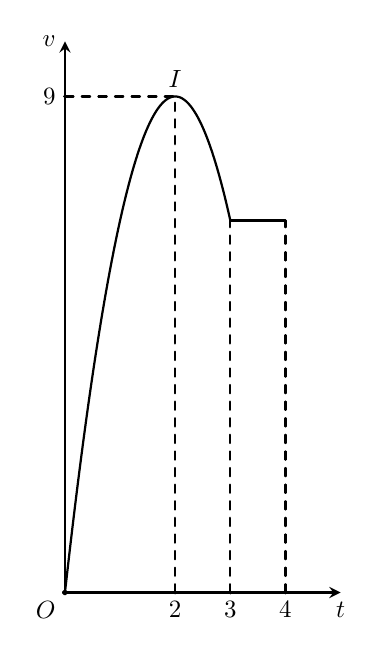
\begin{tikzpicture}[line join=round, line cap=round,>=stealth,thick,scale=0.7]
			
			\draw[->] (0,0)--(5,0) node[below] {$t$};
			\draw[->] (0,0)--(0,10) node[left] {$v$};
			\draw (0,0) node [below left] {$O$} circle(1pt);
			\draw[dashed] (2,0) -- (2,9) -- (0,9) (3,0)--(3,6.75) (4,0)--(4,6.75);
			\draw[samples=200,domain=0:3,smooth,variable=\x] plot (\x,{(-2.25)*(\x)^2 +9*(\x)});
			\draw[thick] (3,6.75)--(4,6.75);
			\fill 
			(0,9) node[left]{$9$} circle(1pt)
			(2,0) node[below]{$2$} circle(1pt)
			(3,0) node[below]{$3$} circle(1pt) 
			(4,0)node[below]{$4$} circle (1pt)
			(2,9)node[above]{$I$};
	\end{tikzpicture}}
	\choiceTF
	{\True Vận tốc lớn nhất của chuyển động là $9$ (km/h)}
	{\True $v(t)=-\dfrac{9}{4}t^2+9t$, với $0\leq t\leq 3$}
	{$v(t)=\dfrac{27}{4}t$, với $3\leq t\leq 4$}
	{\True Quãng đường vật di chuyển được trong 4 giờ là $27$ km}
	\loigiai{		
		\begin{itemchoice}
			\itemch Đúng. Dựa vào đồ thị hàm số ta có $\max\limits_{\left[0;4\right]}v=9$ khi $t=2$ h.
			\itemch Đúng. Với $0\leq t\leq 3$ ta có đồ thị vận tốc là một parabol. Vì parabol có đỉnh $I\left(2;9\right)$ nên parabol có phương trình dạng $y=a\left(t-2\right)^2+9$.\\
			Ta lại có parabol luôn đi qua gốc tọa độ nên $0=a(0-2)^2+9\Leftrightarrow a=-\dfrac{9}{4}$.\\
			Khi đó $y=-\dfrac{9}{a}\left(t-2\right)^2+9\Leftrightarrow y=-\dfrac{9}{4}t^2+9t$.
			\itemch Sai. Với $3\leq t\leq 4$ ta có đồ thị vận tốc là một đường thẳng song song với trục hoành nến $v=c$ với $c=v(3)=-\dfrac{9}{4}\cdot 3^2+9\cdot 3=\dfrac{27}{4}$.\\
			Vậy $y=\dfrac{27}{4}$ với $3\leq t\leq 4$.
			\itemch Đúng. Trong 4 giờ đầu vật chia thành 2 giai đoạn chuyển động.\\
			Giai đoạn 1, trong 3 giờ đầu ta có $s(t)=\displaystyle\int \left(-\dfrac{9}{4}t^2+9t\right)\mathrm{d}t=-\dfrac{3}{4}t^3+\dfrac{9}{2}t^2+c$.\\
			Vì $s(0)=0$ nên $c=0$. Suy ra, $s_{1}=s(3)=\dfrac{81}{4}$ km.\\
			Giai đoạn 2, từ giờ thứ 3 đến giờ thứ 4, ta có $s(t)=\displaystyle\int \dfrac{27}{4}\mathrm{d}t=\dfrac{27}{4}t+c'$. Vì $s(3)=\dfrac{81}{4}$ nên $c'=0$.\\ Suy ra, $s_2=s(4)-s(3)=\dfrac{27}{4}$.\\
			Vậy $s=s_1+s_2=27$ km.
		\end{itemchoice}
	}
\end{ex}

% từ: cau-hoi/lop12/2D4_Nguyen_ham_tich_phan/2D4-2-1_Cong_thuc_ly_thuyet.tex
\begin{bt}%[2D4H2-1]%[ma:833aa1d6]
	Biết $F(x)$ là một  nguyên hàm của hàm số $f(x)=\sin x$ và $F(0)=1$. Tính $F \left(\dfrac{\pi}{2}\right)$.
	 \shortans{2}
	\loigiai{Vì $F(x)$ là một nguyên hàm của hàm số $f(x)=\sin x$ nên 
		$$F\left(\dfrac{\pi}{2}\right)-F(0)=\displaystyle \int_{0}^{\frac{\pi}{2}} f(x)  \mathrm{\,d}x.$$
		Do đó $F\left(\dfrac{\pi}{2}\right)=F(0)+ \displaystyle \int_{0}^{\frac{\pi}{2}}  f(x) \mathrm{\,d}x=1+\displaystyle \int_{0}^{\frac{\pi}{2}} \sin x \mathrm{\,d}x=1+1=2$.
	} 
\end{bt}

% từ: cau-hoi/lop12/2D4_Nguyen_ham_tich_phan/2D4-2-2_Tich_phan_co_ban_da_thuc_phan_thuc.tex
\begin{bt}%[2D4C2-2]%[ma:efa45eee]
% nguon: Archive/SP-4Phan-Dot3/Data/CD_2-OTGK2-De01.tex #4456

	Cho hai đường tròn $(O_1;10)$ và $(O_2;6)$ cắt nhau tại hai điểm $A$, $B$ sao cho $AB$ là một đường kính của đường tròn $(O_2;6)$. Gọi $(D)$ là hình phẳng được giới hạn bởi hai đường tròn (ở ngoài đường tròn lớn, phần được gạch chéo như hình vẽ). Quay $(D)$ quanh trục $O_1 O_2$ ta được một khối tròn xoay. Tính thể tích $V$ của khối tròn xoay được tạo thành.
\begin{center}
\begin{tikzpicture}[scale=0.75, font=\footnotesize, line join=round, line cap=round, >=stealth]
	\draw (-{sqrt(13)},0)--(5,0); % Vẽ trục hoành
	% Vẽ tâm O1 và O2
	\fill[black] (0,0) circle (1pt) node[below] {$O_1$};
	\fill[black] (3,0) circle (1pt) node[below left] {$O_2$};
	% Vẽ đường tròn c1 và c2
	\draw[name path=c1] (0,0) circle[radius=sqrt(13)];
	\draw[name path=c2] (3,0) circle (2);
	% Tìm và nối giao điểm A và B
	\path [name intersections={of=c1 and c2, by={A, B}}];
	\draw (A)--(B);
	% Vẽ các điểm A và B
	\foreach \x/\g in {A/70,B/-70}
	\fill[black] (\x) circle (1pt) ($(\g:3mm)+(\x)$) node {$\x$};
	% Vẽ điểm C
	\draw (5,0) node[right] {$C$};
	\fill[black] (5,0) circle (1pt);
	% Tô màu miền giới hạn bởi hai cung AB của O1 và O2
	\fill[opacity=.8,pattern=north west lines] 
	(B) arc ({-asin(2/sqrt(13))}:{asin(2/sqrt(13))}:{sqrt(13)}) % Cung tròn từ B đến A trên O1
	arc (90:-90:{2});  % Cung tròn từ A đến B trên O2
\end{tikzpicture}
\end{center}
	
	\loigiai
	{
		Chọn hệ tọa độ $Oxy$ với $O_2 \equiv O$, $O_2 C \equiv Ox$, $O_2 A \equiv Oy$.\\
		Cạnh $O_1 O_2=\sqrt{O_1 A^2-O_2 A^2}=\sqrt{10^2-6^2}=8 \Rightarrow(O_1)\colon (x+8)^2+y^2=100$.\\
		Phương trình đường tròn $(O_2)\colon x^2+y^2=36$.\\
		Kí hiệu $(H_1)$ là hình phẳng giới hạn bởi các đường $y=\sqrt{100-(x+8)^2}$, trục $Ox$, $x=0$, $x=2$.\\	
		Kí hiệu $(H_2)$ là hình phẳng giới hạn bởi các đường $y=\sqrt{36-x^2}$, trục $Ox$, $x=0$, $x=6$.\\
		Khi đó thể tích $V$ cần tính chính bằng thể tích $V_2$ của khối tròn xoay thu được khi quay hình $(H_2)$ xung quanh trục $Ox$ trừ đi thể tích $V_1$ của khối tròn xoay thu được khi quay hình $(H_1)$ xung quanh trục $Ox$.\\
		Ta có $V_2=\dfrac{1}{2} \cdot \dfrac{4}{3} \pi r^3=\dfrac{2}{3} \pi \cdot 6^3=144 \pi$.\\
		Lại có $V_1=\pi \displaystyle\int_0^2 y^2 \mathrm{\,d}x=\pi \displaystyle\int_0^2 [100-(x+8)^2] \mathrm{\,d}x=\dfrac{112 \pi}{3}$.\\
		Do đó $V=V_2-V_1=144 \pi-\dfrac{112 \pi}{3}=\dfrac{320 \pi}{3}$.
	}
\end{bt}

% từ: cau-hoi/lop12/2D4_Nguyen_ham_tich_phan/2D4-2-6_Toan_thuc_te_ap_dung_nguyen_ham.tex
\begin{bt}%[2D4V2-6]%[ma:c4c62c97]
	Cho hàm số $y=f (x)$. Đồ thị hàm số $y=f'(x)$ là đường cong trong hình dưới. Biết rằng diện tích của các phần hình phẳng A và B lần lượt là $S_A=4$ và $S_B=10$. Tính giá trị của $f (3)$, biết giá trị  của $f(0)=2$.
	\begin{center}
		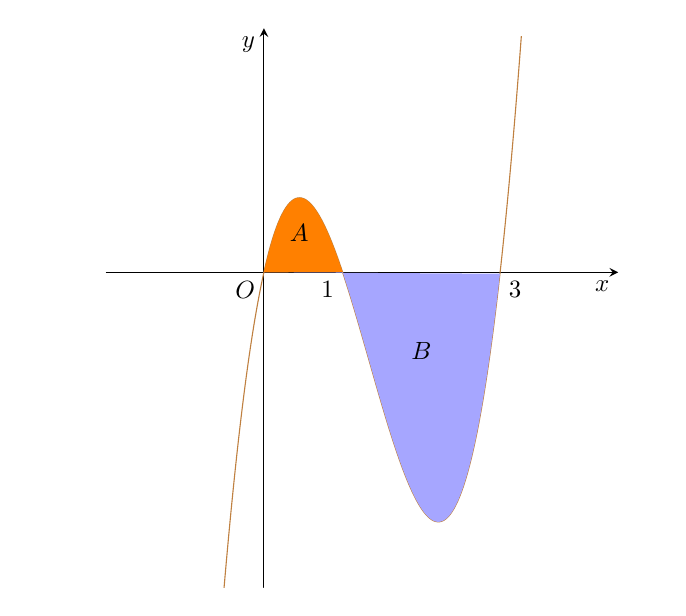
\begin{tikzpicture}[line join=round,line cap=round,>=stealth]
				\tikzset{every  node/.style={scale=0.9}}
				\draw[->] (-2,0)--(4.5,0) node[below left]  {$x$};
				\draw[->] (0,-4)--(0,3.1) node[below left]  {$y$};
				\draw (0,0) node [below left]  {$O$};
				\node at (1,0)  [below left]{$1$};
				\node at (3,0) [below right]{$3$}; 
				\begin{scope}
					\clip (-3,-4) rectangle  (5,3);
					 \draw[brown,samples=200,domain=-1:4,smooth,variable=\x] plot (\x,{1.5*((\x)^3)+-6*((\x)^2)+4.5*(\x)+0});
				\end{scope}
				\fill[orange!100!black!100!] (0,0)--plot[domain=0:1,samples=200] (\x,{1.5*((\x)^3)+-6*((\x)^2)+4.5*(\x)+0})--cycle; 
				\node at (0.45,0.5) {$A$}; 
				\fill[blue!50!white!70!] (0,0)--plot[domain=1:3,samples=200]  (\x,{1.5*((\x)^3)+-6*((\x)^2)+4.5*(\x)+0})--cycle;
				\node at (2,-1) {$B$}; 
			\end{tikzpicture}
	\end{center}
	 \shortans{-4}
	 \loigiai{
		Hình phẳng $A$ được giới hạn bởi đồ thị hàm số $y=f'(x)$, trục hoành $y=0$, trục  tung $x=0$ và đường thẳng $x=1$ nên diện tích hình phẳng $A$ là\\
		\[S_A=\displaystyle\int_0^1 |f'(x)| \mathrm{\,d}x=\displaystyle\int_0^1 f'(x) \mathrm{\,d}x=f(1)-f(0)\] 
		Suy  ra $f(1)=S_A+f(0)=4+2=6$.\\
		Hình phẳng $B$ được giới hạn bởi đồ thị hàm số $y=f'(x)$, trục hoành $y=0$, đường thẳng $x=1$ và đường thẳng $x=3$ nên diện tích hình phẳng $B$ là 
		\[S_B=\displaystyle\int_1^3 |f'(x)|  \mathrm{\,d}x=-\displaystyle\int_1^3 f'(x) \mathrm{\,d}x=-[f(3)-f(1)]=-f(3)+f(1).\]
		Suy  ra $f(3)=f(1)-S_B=6-10=-4$.\\
	Vậy $f  (3)=-4$.}
\end{bt}

% từ: cau-hoi/lop12/2D4_Nguyen_ham_tich_phan/2D4-3-4_The_tich_tinh_theo_mat_cat.tex
\begin{bt}%[2D4H3-4]%[ma:3b69a2ac]
% nguon: Archive/2024/0. [LVH] BG - 12 New - 4in1-20240625T224301Z-001/0. [LVH] BG - 12 New - 4in1/2. [LVH] TEX SGK 12 NEW-20240418T074833Z-001/2. [LVH] TEX SGK 12 NEW/[LVH] SGK-12-KNTT/data/C4/12-c4-bai13-ungdunghinhhoccuatichphan.tex #1163
%[TeX hóa SGK KNTT 12]%[Anh Hoàng Lê]
	Tính thể tích của khối lăng trụ có diện tích đáy bằng $S$ và chiều cao bằng $h$.
	\loigiai{
		\immini{
			Chọn trục $Ox$ song song với đường cao của khối lăng trụ và hai đáy nằm trên hai mặt phẳng vuông góc với $Ox$ tại $x=0$ và $x=h$.
			Mỗi mặt phẳng vuông góc với trục $Ox$ tại điểm có hoành độ bằng $x \,(0 \leq x \leq h)$ cắt khối lăng trụ theo mặt cắt có diện tích không đổi là $S(x)=S$.\\
			Do đó, thể tích của khối lăng trụ là
			$$
			V=\displaystyle\int_0^h S(x) \mathrm{\,d} x=\displaystyle\int_0^h S \mathrm{\,d}x=\left. Sx \bigg|_0^h \right.=Sh.
			$$}{
			\begin{tikzpicture}[line join = round, line cap = round,>=stealth,font=\footnotesize,scale=1]
				\def \h{4}
				\path
				(0,0) coordinate (A)
				(3,0) coordinate (B)
				(4,1) coordinate (C)
				($(A)+(C)-(B)$) coordinate (D)
				($(A)+(-.5,\h)$) coordinate (A')
				($(B)+(-.5,\h)$) coordinate (B')
				($(C)+(-.5,\h)$) coordinate (C')
				($(D)+(-.5,\h)$) coordinate (D')
				($(A)!0.4!(A')$) coordinate (E)
				($(B)!0.4!(B')$) coordinate (F)
				($(C)!0.4!(C')$) coordinate (G)
				($(D)!0.4!(D')$) coordinate (H)
				(1.5,0.5) coordinate (O)
				($(O)+(0,4.2)$) coordinate (h)
				($(O)+(0,6)$) coordinate (t)
				($(O)!0.4!(h)$) coordinate (x)
				;
				%\fill[cyan!50] (E) -- (F) -- (G) -- (H) -- cycle;
				\draw (A) -- (A') (B) -- (B') (C) -- (C') (A) -- (B) -- (C) (A') -- (B') -- (C') -- (D') -- (A') (E) -- (F) -- (G)	(O)--(1.5,-0.5);
				\draw[dashed] (A) -- (D) -- (C) (D) -- (D') (G)  -- (H) -- (E) (O) -- (h)	(A)--(O)	(A')--(h)	(E)--(x); 
				\foreach \x/\g in {A/-90,B/-90,C/0,D/180,A'/180,B'/0,C'/45,D'/90,h/0,x/0,O/0} \fill[black](\x) circle (1pt)+(\g:3mm) node{$\x$};
				\draw[-{Latex[length=3mm,width=2mm]}] (5,5) -- (3,2.5);
				\node[right] at (5,5) {$S(x)$};
				\draw[-{Latex[length=3mm,width=2mm]}] (h) -- (t) node[right] {$x$};
				\node[below] at (1.5,-0.5) {Hình $4.22$};
			\end{tikzpicture}
		}
	}
\end{bt}

% từ: cau-hoi/lop12/2H2_Toa_do_cua_vec_to_trong_khong_gian/2H2-1-3_Tich_vo_huong_va_ung_dung.tex
\begin{ex}%[2H2H1-3]%[ma:6893d83d]
	Cho hình chóp $S.ABCD$ có đáy là hình vuông $ABCD$ cạnh bằng $a$ và các cạnh bên đều bằng $a$. Gọi $M$  và $N$ lần lượt là trung điểm của $AD$ và $SD$. Số đo của góc $(MN, SC)$ bằng
	 \choice
		{$45^\circ$} 
		 {$30^\circ$}
		 {\True $90^\circ$}
		{$60^\circ$} 
	\loigiai{ 
		Ta  có $AC = a\sqrt{2} \Rightarrow AC^2 = 2a^2 = SA^2 + SC^2 \Rightarrow \triangle SAC$ vuông tại $S$.\\
		Khi đó $\overrightarrow{NM}\cdot \overrightarrow{SC} =  \dfrac{1}{2}\overrightarrow{SA}\cdot \overrightarrow{SC} = 0 \Rightarrow \left(\overrightarrow{NM}, \overrightarrow{SC}\right) = 90^\circ$.\\
		Vậy  $(MN,SC) = 90^\circ$.
	 }
\end{ex}

% từ: cau-hoi/lop12/2H2_Toa_do_cua_vec_to_trong_khong_gian/2H2-2-5_Cong_thuc_toa_do_cua_tich_co_huong_va_ung_dun.tex
\begin{ex}%[2H2V2-5]%[ma:c3799b42]
	Cho hình chóp $S.ABC$ có đáy $ABC$ là tam giác vuông cân tại $A$ và $AB = a$, cạnh bên $SA$ vuông góc  với mặt phẳng đáy và $SA = a$. Gọi $D$, $E$, $F$ lần lượt là điểm đối xứng của $A$ qua $C$, của $S$ qua $B$ và của $A$ qua mặt phẳng $(SBC)$. Thể tích của khối tứ diện $ADEF$ bằng
	\choice 
		{\True  $\dfrac{2a^3}{3}$}
		{$\dfrac{2\sqrt{3}a^3}{3}$} 
		{$\dfrac{a^3}{3}$} 
		{$\dfrac{\sqrt{3}a^3}{3}$} 
	 \loigiai{
		\begin{center}
			\begin{tikzpicture}[line join = round,line cap=round,>=stealth,font=\footnotesize,scale=1]
					 \path
						(0,0.7) coordinate  (A)
						(2.1,0) coordinate  (B)
						 (3.55,0.7) coordinate (C)
						 (0,4.65) coordinate (S)
						(1.9,1.76) coordinate (H) 
						(7.1,0.7)  coordinate (D)
						(4.22,-4.65)  coordinate (E)
						(3.78,2.85) coordinate  (F)
						(2.35,2.03) coordinate (N) 
						($(B)! 1/2 !(C)$)  coordinate (M);
					\draw (S)--(A)--(B)--cycle (H)--(F)--(D)--(E)--(A) 
						 (F)--(E)
						 (H)--(S)--(N)
						(S)--(E); 
					\draw [dashed]  (A)--(C)--(B)
						 (C)--(D)
						(A)--(H)--(M) 
						(N)--(C)--(H); 
					\draw[->] (S)--++(0,1) node[left]{$z$}; \draw[->] (D)--++(1,0) node[below]{$y$};  \draw[->] (B)--++(0.7,-0.25) node[below]{$x$};
					\draw pic[draw,angle radius=3mm] {right angle = A--H--M}; 
					\draw pic[draw,angle  radius=3mm] {right angle = S--A--B};
					\draw pic[draw,angle radius=3mm] {right  angle = S--A--C};
					 \draw pic[draw,angle radius=3mm] {right angle = B--A--C};
					 \foreach \p/\r in {A/-90,B/-90,C/-50,S/180,H/90,D/-50,E/-90,F/90}
					\fill (\p) circle (1.2pt)  node[shift={(\r:3mm)}]{$\p$};
				\end{tikzpicture}
		\end{center}
		Chọn hệ trục tọa độ $Axyz$ như hình vẽ  với độ dài vectơ đơn vị bằng $a$, chọn $a=1$ ta được tọa độ các điểm như sau
		$A(0;0;0)$, $B(1;0;0)$,  $C(0;1;0)$, $S(0;0;1) \Rightarrow D(0;2;0)$, $E(2;0;-1)$.\\
		Gọi $H$ là trọng tâm tam giác $SBC \Rightarrow H\left(\dfrac{1}{3}; \dfrac{1}{3}; \dfrac{1}{3}\right)$. Vì tam giác $SBC$ là tam giác đều nên $H$ cũng là trực tâm của tam giác $SBC \Rightarrow AH \perp (SBC) \Rightarrow F$ là điểm đối  xứng của $A$ qua $H \Rightarrow F\left(\dfrac{2}{3}; \dfrac{2}{3}; \dfrac{2}{3}\right)$.\\
		Ta tính được $\overrightarrow{AD}=(0;2;0)$, $\overrightarrow{AE}=(2;0;-1)$, $\overrightarrow{AF}=\left(\dfrac{2}{3};\dfrac{2}{3};\dfrac{2}{3}\right)  \Rightarrow \left[\overrightarrow{AD}, \overrightarrow{AE}\right] = (-2;0;-4)$.\\
		Khi đó $V_{A.DEF} = \dfrac{1}{6}\left|\left[\overrightarrow{AD}, \overrightarrow{AE}\right]\cdot\overrightarrow{AF}\right| =  \dfrac{1}{6}\left|-2\cdot\dfrac{2}{3} + 0\cdot\dfrac{2}{3} - 4\cdot\dfrac{2}{3}\right| = \dfrac{2}{3}$.\\
		Vì độ dài vectơ đơn vị trên trục  bằng $a$ nên ta được thể tích cần tìm là $\dfrac{2a^3}{3}$.
	 }
\end{ex}

% từ: cau-hoi/lop12/2H5_Phuong_trinh_mat_phang_duong_thang_mat_c/2H5-1-6_Goc_giua_hai_mat_phang.tex
\begin{ex}%[2H5V1-6]%[ma:43f8bcc5]
	Cho hình chóp $S.ABC$  có đáy $ABC$ là tam giác đều cạnh $a$ và độ dài cạnh $SA=a$ và vuông góc với $(ABC)$. Góc giữa mặt phẳng $(SAB)$ và mặt phẳng $(SBC)$ là $\alpha$. Khi đó $\tan\alpha$ bằng
	\choice 
		 {$1$}
		 {$\sqrt{3}$}
		 {\True $\sqrt{6}$}
		{$\dfrac{1}{2\sqrt{2}}$} 
	\loigiai{ 
		\begin{center}
			\begin{tikzpicture}[line join = round,line cap=round,>=stealth,font=\footnotesize,scale=1]
					\path 
						(0,1.5)  coordinate (A)
						(1.5,0)  coordinate (B)
						(5,1.5) coordinate (C) 
						 (0,5) coordinate (S)
						($(B)!  1/2 !(C)$) coordinate (H);
					\draw  (A)--(B)--(C)
						 (S)--(A)
						 (S)--(B)
						(S)--(C); 
					\draw[dashed] (H)--(A)--(C); 
					\draw[->] (H)--++(0,5) node[right]{$z$}; \draw[->] (C)--(6,2) node[above]{$x$};  \draw[->] (A)--(-1,1.8) node[above]{$y$};
					\foreach \p/\r in  {A/-130,B/-90,C/-50,S/90,H/-50}
					\fill (\p)  circle (1.2pt) node[shift={(\r:3mm)}]{$\p$};
				\end{tikzpicture}
		\end{center}
		Gắn hệ tọa độ $Oxyz$ như hình  vẽ\\
		Ta có $H(0;0;0)$, $C\left(\dfrac{a}{2};0;0\right)$, $B\left(-\dfrac{a}{2};0;0\right)$, $A\left(0;\dfrac{a\sqrt{3}}{2};0\right)$, $S\left(0;\dfrac{a\sqrt{3}}{2};a\right)$.\\ 
		Ta có $\overrightarrow{AB}=\left(-\dfrac{a}{2}, -\dfrac{a\sqrt{3}}{2},0\right)$, $\overrightarrow{AS}=(0,  0, a)$, $\overrightarrow{BS}=\left(\dfrac{a}{2}, \dfrac{a\sqrt{3}}{2}, a\right)$, $\overrightarrow{BC}=(a, 0, 0)$.\\
		Suy  ra $\overrightarrow{n}_{(SAB)}=\left[\overrightarrow{AB},\overrightarrow{AS}\right]=\left(-\dfrac{a^2\sqrt{3}}{2};-\dfrac{a^2}{2};0\right)$, $\overrightarrow{n}_{(SBC)}=\left[\overrightarrow{BS},\overrightarrow{BC}\right]=\left(0;a^2;-\dfrac{a^2\sqrt{3}}{2}\right)$.\\
		 $\cos\alpha=\left|\dfrac{\overrightarrow{n}_{(SAB)}\cdot\overrightarrow{n}_{(SBC)}}{\left|\overrightarrow{n}_{(SAB)}|\cdot|\overrightarrow{n}_{(SBC)}\right|}\right|=\dfrac{\dfrac{a^4}{2}}{\sqrt{\dfrac{3a^4}{4}+\dfrac{a^4}{4}}\cdot\sqrt{a^4+\dfrac{3a^4}{4}}}=\dfrac{1}{\sqrt{7}}$.\\
		Vậy  $\tan\alpha = \sqrt{\dfrac{1}{\cos^2\alpha}-1} = \sqrt{6}$.
	 }
\end{ex}

% từ: cau-hoi/lop12/2H5_Phuong_trinh_mat_phang_duong_thang_mat_c/2H5-1-6_Goc_giua_hai_mat_phang.tex
\begin{ex}%[2H5V1-6]%[ma:fc21ea8e]
	Cho hình chóp $S.ABCD$ có đáy $ABCD$ là hình vuông cạnh bằng $a$. Cạnh bên $SA=a$  vuông góc với đáy $(ABCD)$. Gọi $M$ là điểm nằm trên cạnh $SD$ sao cho $SM = 2MD$. Hãy tính cosin của góc tạo bởi hai mặt phẳng $(AMC)$ và $(SBC)$?
	 \choice
		{$\dfrac{1}{2}$} 
		{\True  $\dfrac{\sqrt{3}}{2}$}
		 {$\dfrac{2}{\sqrt{5}}$}
		{$1$} 
	 \loigiai{
		\begin{center}
			\begin{tikzpicture}[line join = round,line cap=round,>=stealth,font=\footnotesize,scale=1]
					\draw  (0,0) node[left]{$B (a; 0; 0)$}--(3.5,0) node[below]{$C (a; a; 0)$}--(5.5,1) node[above right]{$D (0; a; 0)$}
						(2,5) node[left]{$S (0;  0; a)$}--(0,0)
						(2,5)--(3.5,0) 
						 (2,5)--(5.5,1)
						 (3.5,0)--($(2,5)!2/3!(5.5,1)$) node[above right]{$M$};
					\draw[dashed]  (0,0)--(2,1) node[above left]{$A (0; 0; 0)$}--(5.5,1)
						(2,5)--(2,1) 
						 ($(2,5)!2/3!(5.5,1)$)--(2,1)--(3.5,0);
					\draw[->] (0,0)--++(-1.3,-0.7) node[left]{$x$};  \draw[->] (2,5)--++(0,1) node[right]{$y$}; \draw[->] (5.5,1)--++(1,0) node[right]{$y$};
				\end{tikzpicture}
		\end{center}
		Chọn hệ trục tọa độ $Oxyz$ sao cho điểm $A \equiv O$, các điểm $B$, $D$, $S$ lần lượt thuộc chiều dương các trục tọa độ $Ox$, $Oy$,  $Oz$. Suy ra tọa độ các điểm như trên hình vẽ.\\
		Do $M$ là điểm nằm trên cạnh $SD$ sao cho $SM = 2MD$ suy ra\\ 
		$\overrightarrow{SM} = \dfrac{2}{3}\overrightarrow{SD} \Rightarrow M\left(0;\dfrac{2a}{3};\dfrac{a}{3}\right)$ $\Rightarrow \heva{&\overrightarrow{AM}=\left(0;\dfrac{2a}{3};\dfrac{a}{3}\right)\\&\overrightarrow{AC}=(a;a;0).}\\ \Rightarrow \left[\overrightarrow{AM},\overrightarrow{AC}\right]=\left(-\dfrac{a^2}{3};\dfrac{a^2}{3};-\dfrac{2a^2}{3}\right)=-\dfrac{a^2}{3}(1;-1;2)$.\\  Ta có $\heva{&\overrightarrow{SB}=(a;0;-a)\\&\overrightarrow{SC}=(a;a;-a)}\Rightarrow \left[\overrightarrow{SB},\overrightarrow{SC}\right]=(a^2;0;a^2)=a^2(1;0;1)$.\\
		Chọn vectơ pháp tuyến  của mặt phẳng $(AMC)$ là $\overrightarrow{n}_1 = (1;-1;2)$.\\
		Chọn vectơ pháp tuyến của mặt phẳng  $(SBC)$ là $\overrightarrow{n}_2 = (1;0;1)$.\\
		Khi đó $$\cos\left((AMC),(SBC)\right) = \dfrac{\left|\overrightarrow{n}_1\cdot\overrightarrow{n}_2\right|}{\left|\overrightarrow{n}_1\right|\cdot\left|\overrightarrow{n}_2\right|} = \dfrac{|1\cdot1 + (-1)\cdot0 + 2\cdot1|}{\sqrt{1^2+(-1)^2+2^2}\cdot\sqrt{1^2+0^2+1^2}}= \dfrac{3}{\sqrt{6}\cdot\sqrt{2}} =  \dfrac{\sqrt{3}}{2}.$$
	 }
\end{ex}

% từ: cau-hoi/lop12/2H5_Phuong_trinh_mat_phang_duong_thang_mat_c/2H5-1-6_Goc_giua_hai_mat_phang.tex
\begin{bt}%[2H5H1-6]%[ma:441798af]
	Cho hình chóp $S.ABCD$ có đáy $ABCD$ là hình vuông có độ dài đường chéo bằng $a\sqrt{2}$ và $SA$ vuông góc với mặt phẳng $(ABCD)$. Gọi $\alpha$ là góc giữa hai mặt phẳng $(SBD)$ và $(ABCD)$. Nếu $\tan\alpha = \sqrt{2}$ thì góc giữa hai mặt phẳng $(SAC)$  và $(SBC)$ bằng bao nhiêu độ?
	\shortans{60} 
	\loigiai{ 
		Gọi $I  = AC \cap BD$.\\
		Hình vuông $ABCD$ có độ dài đường chéo bằng $a\sqrt{2}$ suy ra hình  vuông có cạnh bằng $a$.\\
		Ta có $\left((SBD) \cap (ABCD)\right) =  BD$ nên $\left((SBD);(ABCD)\right) = (SI;AI) = \widehat{SIA}$.\\
		$\tan \widehat{SIA} = \dfrac{SA}{AI}  \Rightarrow SA = a$.\\
		 Chọn hệ tọa độ $Oxyz$ như hình vẽ.\\
		\begin{center}
			\begin{tikzpicture}[scale=0.6,font=\footnotesize,>=stealth]
					\path 
						(0,0) coordinate  (A)
						(-2,-2) coordinate (B) 
						 (5,0) coordinate (D)
						 ($(B)+(D)-(A)$) coordinate (C)
						($(A)+(0,3)$)  coordinate (S)
						(intersection of B--D  and A--C) coordinate (I);
					\draw[->]  (D)--(7,0) node[below]{$y$};
					\draw[->]  (B)--(-3,-3) node[below]{$x$};
					\draw[->] (S)--(0,4)  node[left]{$z$};
					 \draw (C)--(D)--(S)--(C)--(B)--(S);
					 \draw[dashed] (S)--(A)--(D)--(B)--(A)--(C);
					 \pic[draw,thin,angle radius=2mm] {right angle = B--A--D};
					\foreach \x/\g in  {A/180,B/-90,C/-100,D/-80,S/170,I/-90}\draw (\x) circle (.04) +(\g:.5) node{\footnotesize$\x$};
				\end{tikzpicture}
		\end{center}
		Ta có $A(0;0;0), B(a;0;0), C(a;0;a), S(0;0;a)$.\\ 
		Khi đó $\overrightarrow{SA} = (0;0;a),\ \overrightarrow{SC}  = (a;0;-a),\ \overrightarrow{SB} = (a;0;-a)$.\\
		Mặt phẳng $(SAC)$ có vectơ pháp  tuyến $\overrightarrow{n}_1 = (-1;0;1)$.\\
		Mặt phẳng $(SBC)$ có vectơ pháp  tuyến $\overrightarrow{n}_2 = (1;0;1)$.\\
		Suy ra $\cos((SAC);(SBC)) = \dfrac{|\overrightarrow{n}_1 \cdot \overrightarrow{n}_2|}{\left|\overrightarrow{n}_1\right|\cdot\left|\overrightarrow{n}_2\right|} = \dfrac{1}{\sqrt{2} \cdot \sqrt{2}} = \dfrac{1}{2} \Rightarrow \widehat{((SAC);(SBC))}  = 60^\circ$.
	 }
\end{bt}

% từ: cau-hoi/lop12/2H5_Phuong_trinh_mat_phang_duong_thang_mat_c/2H5-2-4_Vi_tri_tuong_doi_giua_hai_duong_thang.tex
\begin{ex}%[2H5H2-4]%[ma:d2d52ae9]
	Cho hình lập phương $ABCD.A_1B_1C_1D_1$ cạnh bằng $a$. Khoảng  cách giữa $A_1B$ và $B_1C$ bằng
	 \choice
		{\True $\dfrac{a}{\sqrt{3}}$} 
		 {$\dfrac{a}{\sqrt{6}}$}
		{$a\sqrt{3}$} 
		 {$a\sqrt{6}$}
	\loigiai{ 
		Chọn hệ trục tọa độ sao  cho $
		B_1(0;0;0)$, $ A_1(a;0;0)$, $ C_1(0;a;0)$, $ B(0;0;a)$, $  C(0;a;a)$.\\
		Ta  có $
		\overrightarrow{A_1B} = (-a;0;a)$, $ \overrightarrow{B_1B} = (0;0;a)$,  $ \overrightarrow{B_1C} = (0;a;a)$.
		 $$
		\left[\overrightarrow{A_1B}, \overrightarrow{B_1C}\right] 
		= (-a^2;-a^2;-a^2)=a^2 (-1;-1;-1). 
		$$ 
		 $$
		\left[\overrightarrow{A_1B}, \overrightarrow{B_1C}\right] \cdot \overrightarrow{B_1B}  = a^2(-1;-1;-1) \cdot (0;0;a) = -a^3.
		 $$
		$$ 
		\Rightarrow \mathrm{d}\left(A_1B, B_1C\right) =  \dfrac{a^3}{\sqrt{(-a)^2 + (-a)^2 + (-a)^2}\cdot \sqrt{a^2}} = \dfrac{a}{\sqrt{3}}.
		$$ 
	} 
\end{ex}

% từ: cau-hoi/lop12/2H5_Phuong_trinh_mat_phang_duong_thang_mat_c/2H5-2-4_Vi_tri_tuong_doi_giua_hai_duong_thang.tex
\begin{ex}%[2H5V2-4]%[ma:fa2c804c]
	Cho hình chóp $S.ABCD$ có đáy $ABCD$ là hình vuông cạnh $a$. Cạnh bên $SA$ vuông góc với đáy. Góc giữa $SC$ và mặt đáy bằng $45^\circ$. Gọi $E$ là trung điểm $BC$. Tính khoảng cách  giữa hai đường thẳng $DE$ và $SC$.
	\loigiai{ 
		Do tam giác $SCA$ vuông tại $A$, góc $\widehat{SCA} = 45^\circ$ nên 
		 $$
		SA = AC = a\sqrt{2}, \quad SC = 2a,\quad SB  = SD = a\sqrt{3}.
		$$ 
		Chọn hệ trục tọa độ $Oxyz$ sao cho $Ox$, $Oy$, $Oz$ lần lượt trùng  với các tia $AB$, $AD$, $AS$.\\
		Tọa độ các  điểm
		$ 
		D(0; a; 0)$, $E\left(a; \dfrac{a}{2}; 0\right)$, $C(a; a; 0)$, $ S\left(0; 0;  a\sqrt{2}\right).
		$ 
		\begin{center}
			\tdplotsetmaincoords{70}{110} 
			\begin{tikzpicture}[tdplot_main_coords,scale=1.4]
					\coordinate (A) at (0,0,0); 
					\coordinate (B) at (3,0,0); 
					 \coordinate (D) at (0,3,0);
					\coordinate (C)  at (3,3,0);
					\coordinate (S) at (0,0,3.24); 
					\coordinate (E) at ($(B)!0.5!(C)$); 
					\coordinate (M)  at ($(S)!0.5!(B)$);
					\draw[dashed]  (B) -- (A) -- (D);
					 \draw (B) -- (C) -- (D);
					 \draw[dashed] (S) -- (A);
					\draw (S) -- (B); 
					\draw  (S) -- (D);
					\draw (S) --  (C);
					\draw[dashed] (M) --  (D) -- (E);
					\draw (S) --  (C);
					\draw  (S) -- (M);
					\draw (B) -- (M)  -- (E);
					\node at (A) [below]  {$A$};
					\node at (B) [below right] {$B$}; 
					 \node at (C) [below right] {$C$};
					\node at (D) [below right] {$D$}; 
					 \node at (S) [left] {$S$};
					\node  at (E) [below right] {$E$};
					 \node at (M) [above right] {$M$};
					\draw[->] (B) -- (4.5,0,0) node[below] {$x$}; 
					\draw[->]  (D) -- (0,4.5,0) node[above] {$y$};
					\draw[->] (S)  -- (0,0,4) node[above] {$z$};
					\fill  (A) circle (1pt);
					 \fill (B) circle (1pt);
					\fill (C) circle  (1pt);
					 \fill (D) circle (1pt);
					\fill (S)  circle (1pt);
					 \fill (E) circle (1pt);
					\fill  (M) circle (1pt);
				\end{tikzpicture}
		\end{center}
		Ta  có
		$ 
		\overrightarrow{DE} = \left(a, -\dfrac{a}{2}, 0\right)$, $ \overrightarrow{SC} = \left(-a, -a, a\sqrt{2}\right)$, $ \overrightarrow{DC} =  (a, 0, 0)$.
		\begin{eqnarray*}
			& & \left[\overrightarrow{DE}, \overrightarrow{SC}\right] = 
			\left(-\dfrac{a^2\sqrt{2}}{2}; -a^2\sqrt{2};  -\dfrac{3a^2}{2} \right).\\
			& & \left[\overrightarrow{DE}, \overrightarrow{SC}\right] \cdot \overrightarrow{DC} = \left(-\dfrac{a^2\sqrt{2}}{2}; -a^2\sqrt{2}; -\dfrac{3a^2}{2} \right)  \cdot (a; 0; 0) = -\dfrac{a^3\sqrt{2}}{2}.\\
			&\Rightarrow&\mathrm{d}(DE, SC) = \dfrac{\left|\left[\overrightarrow{DE}, \overrightarrow{SC}\right] \cdot \overrightarrow{DC}\right|}{\left|\left[\overrightarrow{DE}, \overrightarrow{SC}\right]\right|} = \dfrac{\dfrac{a^3\sqrt{2}}{2}}{\sqrt{\left(\dfrac{a^2\sqrt{2}}{2}\right)^2 + \left(a^2\sqrt{2}\right)^2 + \left(\dfrac{3a^2}{2}\right)^2}}  = \dfrac{a\sqrt{38}}{19}.
		\end{eqnarray*}
	} 
\end{ex}

% từ: cau-hoi/lop12/2H5_Phuong_trinh_mat_phang_duong_thang_mat_c/2H5-2-4_Vi_tri_tuong_doi_giua_hai_duong_thang.tex
\begin{bt}%[2H5V2-4]%[ma:85b1b6f3]
	Cho hình chóp $S.ABCD$ có đáy $ABCD$ là hình vuông cạnh bằng $10$. Cạnh bên $SA$ vuông góc với mặt phẳng $(ABCD)$ và $SC = 10\sqrt{5}$. Gọi $M, N$ lần lượt là trung điểm của $SA$ và $CD$. Tính khoảng cách $d$ giữa  $BD$ và $MN$.
	 \loigiai{
		Xét tam giác vuông $SAC$ có 
		$$ 
		SA = \sqrt{SC^2 - AC^2} = \sqrt{500  - 200} = 10\sqrt{3}.
		$$ 
		Chọn hệ  trục tọa độ như hình vẽ sao cho\\
		$ 
		A(0;0;0)$, $  B(10;0;0)$, $ D(0;10;0)$, $ C(10;10;0)$, $ S\left(0;0;10\sqrt{3}\right)$, $
		M(0;0;5\sqrt{3})$, $N(5;10;0).$ 
		\begin{center}
			\tdplotsetmaincoords{70}{110} 
			\begin{tikzpicture}[tdplot_main_coords,scale=1]
					\coordinate (A) at (0,0,0); 
					\coordinate  (B) at (4,0,0);
					\coordinate (C)  at (4,4,0);
					\coordinate (D) at (0,4,0); 
					\coordinate  (S) at (0,0,4);
					\draw[dashed] (A) --  (D);
					\draw[dashed] (A)  -- (B);
					\draw  (B) -- (C) -- (D);
					\draw[dashed] (S) --  (A);
					\draw  (S) -- (B);
					 \draw (S) -- (C);
					\draw (S) --  (D);
					\node  at (A) [left] {$A$};
					\node at (B) [above  left] {$B$};
					\node at (C) [below right]  {$C$};
					\node at (D) [above right]  {$D$};
					\node at (S) [left]  {$S$};
					\coordinate (M)  at ($(S)!0.5!(A)$);
					\coordinate (N) at ($(C)!0.5!(D)$); 
					\fill  (M) circle (1pt) node[left] {$M$};
					\fill (N) circle (1pt) node[right] {$N$}; 
					\draw[dashed] (B) -- (D); 
					\draw[dashed] (M) --  (N);
					\draw[->] (B) -- (5,0,0)  node[right] {$x$};
					\draw[->] (D) -- (0,5,0) node[above] {$y$}; 
					\draw[->]  (S) -- (0,0,5) node[above] {$z$};
				\end{tikzpicture}
		\end{center}
		Ta có 
		\begin{itemize}
			\item $\overrightarrow{MN}  = (5;10;-5\sqrt{3}) \Rightarrow \overrightarrow{u}_1 = (1;2;-\sqrt{3})$.
			\item $ \overrightarrow{BD} =  (-10;10;0) \Rightarrow \overrightarrow{u}_2 = (-1;1;0)$.
		\end{itemize}
		 Ta có
		 $$
		 \left[\overrightarrow{u}_1, \overrightarrow{u}_2\right] =
		\left(\sqrt{3};  \sqrt{3}; 3\right)
		\quad  \text{ và} \quad \overrightarrow{ND} = (-5;0;0).
		$$ 
		$$ 
		\Rightarrow  \mathrm{d}(MN, BD) = \dfrac{\left|\left[\overrightarrow{u}_1, \overrightarrow{u}_2\right] \cdot \overrightarrow{ND}\right|}{\left|\left[\overrightarrow{u}_1, \overrightarrow{u}_2\right]\right|} = \dfrac{\left|-\sqrt{3} \cdot 5\right|}{\sqrt{3^2 + 3 + 3}} = \dfrac{5\sqrt{3}}{\sqrt{9 + 3 + 3}} = \sqrt{5}.
		$$ 
	 }
\end{bt}

% từ: cau-hoi/lop12/2H5_Phuong_trinh_mat_phang_duong_thang_mat_c/2H5-2-4_Vi_tri_tuong_doi_giua_hai_duong_thang.tex
\begin{bt}%[2H5V2-4]%[ma:116b23aa]
	Cho hình chóp $S.ABCD$ có đáy $ABCD$ là hình vuông cạnh $a$. Cạnh bên $SA$ vuông góc với đáy. Góc giữa $SC$ và mặt đáy bằng  $45^\circ$. Gọi $E$ là trung điểm $BC$. Tính khoảng cách giữa hai đường thẳng $DE$ và $SC$.
	 \loigiai{
		Do tam giác $SCA$ vuông tại $A$,  góc $\widehat{SCA} = 45^\circ$ nên
		$$ 
		SA = AC = a\sqrt{2}, \quad SC = 2a,\quad SB = SD = a\sqrt{3}. 
		 $$
		Chọn hệ trục tọa độ $Oxyz$ sao cho $Ox$, $Oy$, $Oz$  lần lượt trùng với các tia $AB$, $AD$, $AS$.\\
		Tọa  độ các điểm
		 $
		 D(0; a; 0)$, $E\left(a; \dfrac{a}{2}; 0\right)$, $C(a; a; 0)$, $ S\left(0; 0; a\sqrt{2}\right).
		$ 
		\begin{center}
			\tdplotsetmaincoords{70}{110} 
			\begin{tikzpicture}[tdplot_main_coords,scale=1.4]
					 \coordinate (A) at (0,0,0);
					\coordinate (B) at (3,0,0); 
					\coordinate  (D) at (0,3,0);
					\coordinate (C) at (3,3,0); 
					 \coordinate (S) at (0,0,3.24);
					 \coordinate (E) at ($(B)!0.5!(C)$);
					\coordinate (M)  at ($(S)!0.5!(B)$);
					\draw[dashed] (B) --  (A) -- (D);
					\draw (B) -- (C) --  (D);
					 \draw[dashed] (S) -- (A);
					\draw (S) --  (B);
					\draw (S) -- (D); 
					 \draw (S) -- (C);
					 \draw[dashed] (M) -- (D) -- (E);
					 \draw (S) -- (C);
					\draw (S)  -- (M);
					\draw (B) -- (M) --  (E);
					\node at  (A) [below] {$A$};
					 \node at (B) [below right] {$B$};
					\node at (C) [below right] {$C$}; 
					\node at (D)  [below right] {$D$};
					\node at (S)  [left] {$S$};
					 \node at (E) [below right] {$E$};
					 \node at (M) [above right] {$M$};
					\draw[->] (B) --  (4.5,0,0) node[below] {$x$};
					\draw[->] (D)  -- (0,4.5,0) node[above] {$y$};
					 \draw[->] (S) -- (0,0,4) node[above] {$z$};
					\fill (A) circle (1pt); 
					\fill (B) circle (1pt); 
					 \fill (C) circle (1pt);
					\fill (D) circle  (1pt);
					\fill (S) circle  (1pt);
					\fill (E) circle (1pt); 
					\fill (M) circle  (1pt);
				\end{tikzpicture}
		\end{center}
		 Ta có
		 $
		 \overrightarrow{DE} = \left(a, -\dfrac{a}{2}, 0\right)$, $ \overrightarrow{SC} = \left(-a, -a, a\sqrt{2}\right)$, $ \overrightarrow{DC} = (a, 0, 0)$.
		\begin{eqnarray*}
			& & \left[\overrightarrow{DE},  \overrightarrow{SC}\right] =
			\left(-\dfrac{a^2\sqrt{2}}{2}; -a^2\sqrt{2}; -\dfrac{3a^2}{2}  \right).\\
			& & \left[\overrightarrow{DE}, \overrightarrow{SC}\right] \cdot \overrightarrow{DC} = \left(-\dfrac{a^2\sqrt{2}}{2}; -a^2\sqrt{2}; -\dfrac{3a^2}{2} \right)  \cdot (a; 0; 0) = -\dfrac{a^3\sqrt{2}}{2}.\\
			&\Rightarrow&\mathrm{d}(DE, SC) = \dfrac{\left|\left[\overrightarrow{DE},  \overrightarrow{SC}\right] \cdot \overrightarrow{DC}\right|}{\left|\left[\overrightarrow{DE}, \overrightarrow{SC}\right]\right|} = \dfrac{\dfrac{a^3\sqrt{2}}{2}}{\sqrt{\left(\dfrac{a^2\sqrt{2}}{2}\right)^2 + \left(a^2\sqrt{2}\right)^2 + \left(\dfrac{3a^2}{2}\right)^2}} = \dfrac{a\sqrt{38}}{19}.
		\end{eqnarray*}
	 }
\end{bt}

% từ: cau-hoi/lop12/2H5_Phuong_trinh_mat_phang_duong_thang_mat_c/2H5-2-6_Khoang_cach_diem_toi_duong_thang.tex
\begin{ex}%[2H5V2-6]%[ma:c1770f50]
	Cho lăng trụ đứng $ABC.A'B'C'$ có đáy $ABC$ là tam giác vuông tại $B$, $AB=a$, $BC=a\sqrt{2}$, $AA'=a\sqrt{3}$. Trên $BB'$ lấy điểm $N$ sao cho $BN = \dfrac{a}{\sqrt{3}}$. Khoảng cách từ $B'$ đến mặt phẳng $(AC'N)$ bằng 
	\choice 
		{\True  $\dfrac{a\sqrt{6}}{2}$}
		 {$a\sqrt{6}$}
		 {$\dfrac{a\sqrt{6}}{6}$}
		{$\dfrac{a\sqrt{6}}{3}$} 
	 \loigiai{
		\begin{center}
			\begin{tikzpicture}[line join = round,line cap=round,>=stealth,font=\footnotesize,scale=1]
					\path 
						(0,1.5)  coordinate (A)
						 (1.5,0) coordinate (B)
						 (5,1.5) coordinate (C)
						(0,5) coordinate (A') 
						 (1.5,3.5) coordinate (B')
						(5,5) coordinate (C') 
						($(B')! 2/3  !(B)$) coordinate (N);
					\draw  (A)--(B) node[midway,left]{$a$}--(C) node[midway,right]{$a\sqrt{3}$}
						 (A)--(A')
						(B)--(B') 
						(C)--(C') 
						 (A')--(B')--(C')--cycle (A)--(N)--(C')
						(N)--(B)  node[midway,right]{$\dfrac{a}{\sqrt{3}}$};
					 \draw[dashed] (C')--(A)--(C);
					 \draw[->] (A)--(-0.5,2) node[left]{$x$}; \draw[->] (C)--(6,2) node[above]{$y$}; \draw[->] (B')--++(0,3) node[right]{$z$};
					\foreach  \p/\r in {A/180,B/-90,C/-30,A'/90,B'/-40,C'/0,N/-30}
					\fill (\p) circle (1.2pt)  node[shift={(\r:3mm)}]{$\p$};
				\end{tikzpicture}
		\end{center}
		Chọn hệ trục tọa độ như hình vẽ, khi đó  ta có $A(a;0;0)$, $N\left(0;0;\dfrac{a}{\sqrt{3}}\right)$, $C'\left(0;a\sqrt{2};a\sqrt{3}\right)$,
		$B'(0;0;a\sqrt{3})$. $\overrightarrow{AN} = \left(-a;0;\dfrac{a}{\sqrt{3}}\right)$, $\overrightarrow{AC'}  = (-a;a\sqrt{2};a\sqrt{3})$.\\
		Mặt phẳng $(AC'N)$ đi qua $A(a;0;0)$ có vectơ pháp tuyến $\overrightarrow{n}  = \left[\overrightarrow{AN}, \overrightarrow{AC'}\right] = \left(-\dfrac{a^2\sqrt{6}}{3}; \dfrac{2a^2\sqrt{3}}{3}; -a^2\sqrt{2}\right)$ có phương trình
		là $(AC'N)$$\colon$ $-\dfrac{\sqrt{6}}{3}(x-a) +  \dfrac{2\sqrt{3}}{3}y - \sqrt{2}z = 0$.\\
		Khoảng cách $\mathrm{d}\left(B', (AC'N)\right) =  \dfrac{\left|\dfrac{a\sqrt{6}}{3}-a\sqrt{6}\right|}{\sqrt{\dfrac{6}{9}+\dfrac{4}{3}+2}}=\dfrac{a\sqrt{6}}{3}$.
	 }
\end{ex}

% từ: cau-hoi/lop12/2H5_Phuong_trinh_mat_phang_duong_thang_mat_c/2H5-2-6_Khoang_cach_diem_toi_duong_thang.tex
\begin{ex}%[2H5V2-6]%[ma:bff5347e]
	Cho lăng trụ $ABC.A'B'C'$ có tam giác $ABC$  đều cạnh bằng $2a$. Hình chiếu vuông góc của $A'$ lên mặt phẳng $(ABC)$ trùng với trung điểm $M$ của $BC$. Biết góc tạo bởi $A'B$ và mặt đáy bằng $60^\circ$. Khoảng cách từ $B$ đến mặt phẳng $(AB'C)$ là
	\choice 
		 {$\dfrac{a\sqrt{7}}{7}$}
		 {$\dfrac{2a\sqrt{7}}{7}$}
		{\True  $\dfrac{2a\sqrt{39}}{13}$}
		{$\dfrac{a\sqrt{39}}{13}$} 
	 \loigiai{
		\begin{center}
			\begin{tikzpicture}[line join = round,line cap=round,>=stealth,font=\footnotesize,scale=1]
					\path 
						(0,1) coordinate (A) 
						(1,0)  coordinate (B)
						(4.5,1) coordinate  (C)
						(2.8,5) coordinate  (A')
						(3.8,4) coordinate  (B')
						 (7.3,5) coordinate (C')
						($(B)! 1/2 !(C)$) coordinate  (M);
					\draw (A)--(B)--(C) 
						(A')--(B')--(C')--cycle  (A)--(A')
						(B)--(B') 
						(C)--(C') 
						(A')--(B); 
					\draw[dashed]  (A)--(C)
						 (A')--(M)--(A);
					\draw[line  width=0.5pt] (A)--(B')--(C);
					\draw[fill=gray!70,dashed,opacity=0.4]  (A)--(B')--(C)--cycle;
					\draw pic[draw,angle radius=3mm] {right angle = A'--M--C}; 
					\draw (M)  node[below right]{$M\equiv O$};
					\draw [->]  (A')--++(0,1) node[right]{$z$}; \draw [->] (A)--++(-1,0.2) node[below]{$x$}; \draw [->] (B)--++(-1,-0.3) node[below]{$y$};
					\foreach \p/\r  in {A/200,B/-90,C/0,A'/130,B'/-30,C'/0}
					\fill (\p)  circle (1.2pt) node[shift={(\r:3mm)}]{$\p$};
				\end{tikzpicture}
		\end{center}
		Góc giữa $A'B$ và mặt phẳng  $(ABC)$ là góc $\widehat{A'BM}=60^{\circ}$.\\
		Ta có $A'M =  BM\cdot\tan 60^{\circ} = a\sqrt{3}$; $AM = AB\cdot\sin 60^{\circ} = 2a\cdot\dfrac{\sqrt{3}}{2} = a\sqrt{3}$.\\
		Đặt hệ trục tọa $Oxyz$ như hình vẽ. Coi $a=1$ khi đó $A(\sqrt{3};0;0)$, $B(0;1;0)$,  $C(0;-1;0)$,
		$A'(0;0;\sqrt{3})$. Gọi $B'(x_0;y_0;z_0)$, $\overrightarrow{A'B'} = (x_0;y_0;z_0-\sqrt{3})$, $\overrightarrow{AB} = (-\sqrt{3};1;0)$.\\ 
		Vì $\overrightarrow{A'B'} = \overrightarrow{AB}$ nên $\heva{&x_0 = -\sqrt{3}\\& y_0  = 1 \\ &z_0=\sqrt{3}} \Rightarrow B'(-\sqrt{3};1;\sqrt{3})$.\\
		Ta có $\heva{&\overrightarrow{AC} =  (-\sqrt{3};-1;0)\\&\overrightarrow{AB'} = (-2\sqrt{3};1;\sqrt{3})} \Rightarrow \left[\overrightarrow{AC}, \overrightarrow{AB'}\right] = (-\sqrt{3};3;-3\sqrt{3}) \Rightarrow \overrightarrow{n}=(1;-\sqrt{3};3)$ là vectơ pháp tuyến của $\mathrm{mp}(ACB')$. \\
		Phương trình mặt phẳng $(ACB')$ là $x-\sqrt{3}y+3z-\sqrt{3}=0$.\\ 
		$\Rightarrow \mathrm{d}\left(B, (ACB')\right)  = \dfrac{\left|0+\sqrt{3}\cdot1+0-\sqrt{3}\right|}{\sqrt{1+3+9}} = \dfrac{2\sqrt{39}}{13}$.\\
		Vậy khoảng cách  từ $B$ đến $(AB'C)$ là $\dfrac{2a\sqrt{39}}{13}$.
	 }
\end{ex}
